%!TEX program = xelatex
\documentclass [PhD] {uclathes}
\usepackage{siunitx}
\usepackage[toc,page]{appendix}
\usepackage[noprefix]{nomencl}
\usepackage{lscape}
\makeglossary \makeindex
\usepackage[table]{xcolor}
\usepackage[tbtags]{amsmath}
\usepackage{placeins}
\usepackage{amsbsy}
\usepackage{color}
\usepackage[superscript,biblabel]{cite}
\usepackage{amssymb}
\usepackage{longtable}
\usepackage{verbatim}
\usepackage{chngpage}
 \ifx\pdfoutput\undefined
   \usepackage[dvips]{graphicx}
   \else
   \usepackage[pdftex]{graphicx}
   \pdfcompresslevel=9
   \fi
\usepackage{array}
\usepackage{float}
\usepackage[colorlinks,citecolor=red,linkcolor=blue]{hyperref}
\usepackage{subfiles}
\usepackage{xltxtra} % Extra customizations for XeLaTeX
\usepackage{tabularx, multirow, booktabs}
\newcommand{\otoprule}{\midrule[\heavyrulewidth]}
\usepackage{subcaption}

\usepackage{textcomp}%it was suggested online to load this before gensymb to get rid of an annoying error
\usepackage{gensymb}
\setcounter{secnumdepth}{5}
\setcounter{tocdepth}{2}
%\linespread{1.6}%double line (1.6%) spacing, for one & half use {1.3}
\usepackage{cleveref}
\usepackage{mathrsfs}
\usepackage{mhchem}

% \usepackage[version=3]{mhchem}
% \usepackage{chemmacros}
%\usepackage{breqn}

%vanlew-environments

% time derivative
\newcommand{\dt}[1]{
\frac{\mathrm{d}{#1}}{\mathrm{d}t}}
\newcommand{\ddt}[1]{
\frac{\mathrm{d}^2{#1}}{\mathrm{d}t^2}}

% partial derivative (with optional numerator and required denominator)
\newcommand{\pder}[2][]{\frac{\partial#1}{\partial#2}}

% custom vector notation
\renewcommand{\vec}[1]{\mathbf{#1}}




\newcommand{\lit}{Li$_2$TiO$_3$~}
\newcommand{\lis}{Li$_4$SiO$_4$~}
\sisetup{locale = US}


% Dimensionless numbers
\newcommand{\Nu}{\mathrm{Nu}}
\renewcommand{\Re}{\mathrm{Re}}
\renewcommand{\Pr}{\mathrm{Pr}}
\newcommand{\Ra}{\mathrm{Ra}}
\newcommand{\Bi}{\mathrm{Bi}}
\newcommand{\Fo}{\mathrm{Fo}}








                        % personal LaTeX macros


\title          {Shitty Dissertation Title}
\author         {Jon Thomas Van Lew}
\department     {Mechanical Engineering}
\degreeyear     {2015}

\chair{Mohamed Abdou}
\member{Alice Ying}
\member{Pirouz Kavehpour}
\member{Nasr Ghoniem}
\member{Jaime Marian}

%\dedication     {\textsl{To My loved ones \ldots without \\
%                whom I could not find the will\\
%      and courage to do this}}

\acknowledgments {I did it all on my own}

\vitaitem {2005} {B.S., Mechanical Engineering, Cum Laude\\ University of Arizona\\ Tucson, AZ}
\vitaitem {2010} {M.S., Mechanical Engineering \\ University of Arizona \\ Tucson, AZ}

\abstract{It's all crap}

\begin{document}

%%%%%%%%%%%%%%%%%%%%%%%%%%%%%%%%%%%%%%%%%%%%%%%%%%%%%%%%%%%%%%%%%%%%%%%%%
%\makeintropages

%\mymaketitlepages              % Thesis Title Page
%\mymakecopyrightpage           % Copyright Page
%\pagenumbering{roman}
%\setcounter{page}{1}
%\mymakeabstractpage            % Abstract Page
%\mymakesignaturepage           % Committee Member Signature Page
%\setcounter{page}{4}
\tableofcontents               % Table of Contents
%\listoffigures                 % List of Figures
%\listoftables                  % List of Tables
%\chapter*{Nomenclature}

\begin{tabbing}
aaaaaaaaa\= aaaaaaaaa\kill
$a$ \>        lattice parameter, $\AA$\\
$A$ \>        sample cross-sectional area, m$^2$\\
$A_s$ \>        sample surface area, m$^2$\\
$b$ \>        sample thickness, m \\
$Bi$ \>       Biot number (=$hb/k$) \\
$c_p$ \>      specific heat, J/kg$\cdot$K\\
$C$ \>        capacitance, F \\
$D$ \>        electric displacement, C/m$^2$\\
$d_{33}$ \>   piezoelectric coefficient, C/N\\
$\Delta h$ \>  specific phase change enthalpy, J/kg\\
$E$ \>        electric field, V/m\\
$E_{br}$ \>    electrical breakdown field, V/m\\
$E_{c}$ \>    coercive electric field, V/m\\
$f$ \>        frequency, Hz\\
$g$ \>          gravity of Earth (=9.81 m/s$^2$) \\
$h$    \>     heat transfer coefficient, W/m$^{2}$$\cdot$K \\
$k$ \>        thermal conductivity, W/m$\cdot$K\\
$I_p$ \>      electric current, A\\
M$_A$ \>       monoclinic M$_A$ crystal phase \\
M$_B$ \>       monoclinic M$_B$ crystal phase \\
M$_C$ \>       monoclinic M$_C$ crystal phase \\
$mol\%$\>    molar fraction, \% \\
MPB \>         morphotropic phase boundary \\
$N_D$ \>      energy density, J/L\\
$Nu$ \>     Nusselt number \\
O \>       orthorhombic crystal phase \\
$p_c$ \>      pyroelectric coefficient, C/m$^2$$\cdot$K\\
$P$ \>        polarization density, C/m$^2$\\
$P_D$ \>      power density, W/L\\
$P_r$ \> 	  remnant polarization, C/m$^2$\\
$P_s$ \> 	  saturation polarization, C/m$^2$\\
$Q$ \> 	      charge, C \\
$Q_{in}$ \>     thermal energy input per unit volume, J/m$^3$ \\
PE \> 	  pyroelectric element \\
R \>       rhombohedral crystal phase \\
$R$ \> 	      resistance, $\Omega$ \\
$Ra$ \>         Rayleigh number \\
$S$ \>          side length, m \\
$s_{33}$ \>   elastic compliance, m$^{2}$/N \\
$t$ \>        time, s\\
T \>       tetragonal crystal phase \\
$T$ \>        temperature, $^o$C or K\\
$T_{Curie}$ \> Curie temperature, $^o$C\\
$x$ \>	      molar fraction of lead titanate, \%\\
$x_{3}$ \>	  strain in longitudinal direction [=$\int_{T_{C}}^{T} \! \alpha(T) \, \mathrm{d} T$] \\
$-\!\!\!\! V$ \>      volume, m$^3$ \\
$V$\>         voltage, V \\
$V_{1}$\>     voltage across capacitor, V \\
$V_{2}$\>     voltage across resistor, V \\
$W_{in}$ \>     mechanical energy input per unit volume, J/m$^3$ \\
\\

\textbf{Greek symbols} \\
$\alpha$ \>     linear thermal expansion coefficient, K$^{-1}$\\
$\delta$  \>    relative error between experimental data and model predictions, \% \\
$\varepsilon_{o}$  \> vacuum permittivity (= 8.854x10$^{-12}$ F/m) \\
$\varepsilon_{r}$ \>  relative permittivity  \\
$\eta$ \>          material efficiency, \% \\
$\nu$ \>        kinematic viscosity, m$^2$/s \\
$\rho$     \>     density, kg/m$^3$ \\
$\sigma$   \>     elastic stress, Pa \\
$\tau$$_{t}$     \>   thermal characteristic time constant, s\\
$\tau_{ij}$ \>   duration of process $i$-$j$, s\\
\\

\textbf{Subscripts} \\
$avg$ \>  refers to average \\
$b$ \>      refers to bias \\
$cold$ \>  refers to cold \\
$eff$ \>   refers to effective \\
$f$ \>      refers to fluid \\
$H$ \>    refers to high \\
$hot$ \>   refers to hot \\
$L$ \>    refers to low \\
$max$  \>   refers to maximum \\
$PE$ \>    refers to pyroelectric element \\
\end{tabbing}





%\printglossary                 % Nomenclature Page
%\mymakeacknowledgmentspage     % Acknowledgments Page
%\mymakevitapages               % Vita Page
%\mytitlefinish                 % Start a New Page for Chapter 1.

%%%%%%%%%%%%%%%%%%%%%%%%%%%%%%%%%%%%%%%%%%%%%%%%%%%%%%%%%%%%%%%%%%%%%%%%%%%
%\pagenumbering{arabic}
%\setcounter{page}{1}

% Reference sections
%%%%%%%%%%%%%%%%%%%%%%%%%%%%%%%%%%%%%%%%%%
\chapter{Introduction} \label{sec:introduction}
%%%%%%%%%%%%%%%%%%%%%%%%%%%%%%%%%%%%%%%%%%
The controlled, sustained thermonuclear fusion of light elements can serve as the ultimate energy source on Earth; it is inexhaustible (on our planetary scales), produces none of the greenhouse gases that are altering our climate, and avoids many of the dangers of nuclear fission. Overcoming the engineering obstacles to tame the fusion reaction is the greatest technological challenge of our generation. %A recently-published book by Dr. Francis Chen provides an excellent coverage of the basics of fusion energy, the reactions, our present understanding of the fusion plasma, and the role fusion energy can play in the global energy market.\cite{Chen2011} 

In this dissertation, I will begin by presenting an extremely brief summary on the background of general fusion technology -- necessary for establishing a common language that will be used in the rest of the document. I'll then give slightly more background on some fusion nuclear technology that are immediately relevant to the research I have performed, specifically the breeder blanket of a fusion reactor.

\section{The Basics of Nuclear Fusion and Tritium Breeding}\label{sec:fusion-basics}

The fusion reaction chosen for the first demonstrable fusion power plants involves the two hydrogen isotopes of deuterium and tritium. The deuterium-tritium (DT) reaction has a high reaction probability at the lowest ion temperature and a high energy yield. Alternative fusion reactions of two deuterium atoms or a deuterium atom with helium-3 are advantageous in other regards, such as no radioactive byproducts or fuel availability, but their relatively-higher ion temperature preclude them from current feasibility.\cite{abdou} The DT reaction proceeds as
\begin{align}
	\mathrm{D} + \mathrm{T}&\xrightarrow{}\ ^4\mathrm{He}+\mathrm{n}+17.58\ \text{MeV} \label{eq:dt-reaction}
\end{align}

Of the two isotopes fused, deuterium ($D$, or $^2$H) is a stable isotope and is naturally occurring in an average abundance of 0.015 mole percent in water on Earth. To demonstrate just how plentiful deuterium is as a fuel source, there is approximately 100 million billion kilograms of deuterium in the Earth's oceans. If all energy on Earth were produced from DT fusion power plants, there would be enough deuterium to outlast the lifetime of our sun. It is safe to say we will not exhaust our deuterium sources on Earth.

Tritium ($T$, or $^3$H), however, is radioactive with a half-life of only about 12 years; any naturally occurring tritium decays at such a rapid pace it will never accumulate to an appreciable amount on Earth. If tritium is to be used as a fuel in a fusion power plant, it must be generated artificially. In-situ generation of tritium in a fusion reactor is possible with the assistance of lithium. Natural lithium will interact with neutrons as
\begin{subequations}\label{eq:lithium-t}
\begin{align}
	\mathrm{n} + \ ^7\mathrm{Li} &\xrightarrow \ \mathrm{n}+\alpha + \mathrm{T} -2.47\ \text{MeV}\label{eq:li7-t}\\
	\mathrm{n} + \ ^6\mathrm{Li} &\xrightarrow \  \alpha + \mathrm{T} +4.78\ \text{MeV} \label{eq:li6-t}
\end{align}
\end{subequations}
using the common short-hand of $\alpha$ in place of the helium nucleus. The cross-sections of the lithium reactions are given in Fig.~\ref{fig:li-xsects}. Of note in Fig.~\ref{fig:li-xsects} is the exothermic lithium-6 reaction (a neutron of any energy will incite the transmutation) and the threshold energy required of the incident neutron to incite the endothermic lithium-7 reaction. The exothermic reaction, in addition to producing tritium, is also the source of energy that will ultimately generate the electricity of the fusion power plant.

\begin{figure}[ht]
	\centering
	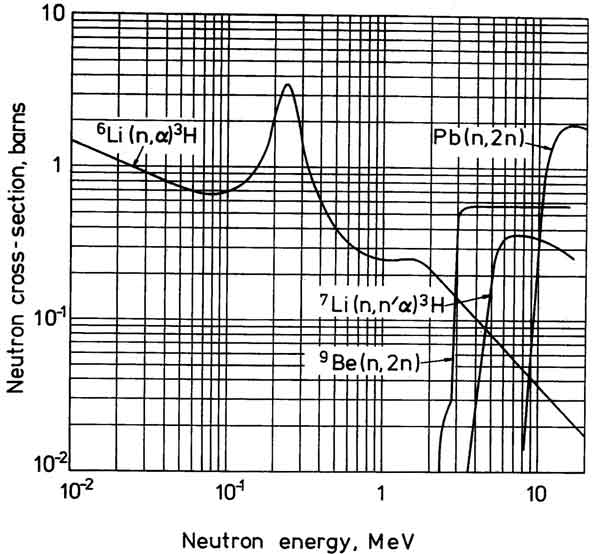
\includegraphics[width=\singleimagewidth]{chapters/figures/breeding_xsecs} 
	\caption{Cross-sections of various blanket materials. Note the threshold for the $^7$Li and neutron multiplying reactions.}
	\label{fig:li-xsects}
\end{figure}

Fortunately, lithium, like deuterium, is quite abundant on Earth. There is enough lithium accessible in the Earth's crust to generate tritium for 30 million years worth of DT reactions.\cite{Chen2011}. Thus lithium is an excellent candidate for generating the tritium necessary to self-sustain the fusion reaction in a power plant. Fusion reactor designs include so-called tritium breeding blankets which surround the plasma volume with lithium, however the form of lithium as it exists in the breeding blanket is a source of continued research.



At present there are two main concepts for tritium breeder designs: those containing liquid or solid lithium. Many of the functional requirements are similar between the two designs but their implementations are quite different. While much research has been -- and continues to be -- performed on the liquid breeder design (for examples, see Refs.~\cite{Hartmann1937,Hunt2006,Shercliff1953,Sommeria1982,Xv1937,Alfve1942}), the work of this dissertation focuses solely on the reference solid breeder design. In the next section, while introducing the breeding blanket, I will refer to the blanket almost exclusively as simply ``solid breeder'' though it should be understood that many of the generic features and requirements of the solid breeder are shared with its sister design, the liquid breeder.

\subsection{Breeding Blanket for Fusion Reactors}


\begin{figure}[ht]
	\centering
	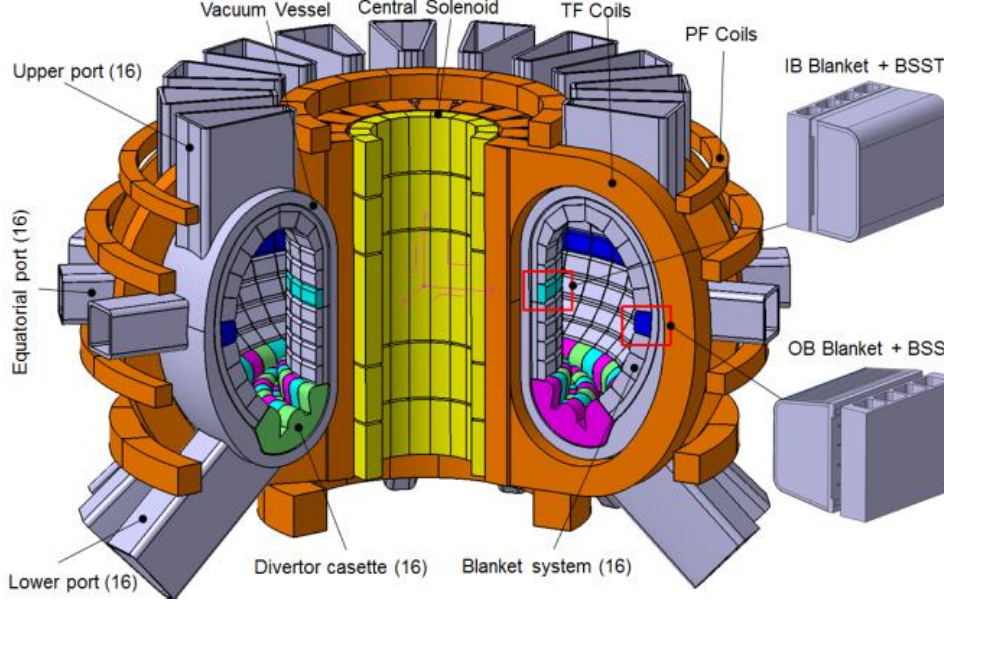
\includegraphics[width=1\textwidth]{chapters/figures/demo} 
	\caption{An example design of a DEMO reactor with solid breeder blankets shown as inboard (IB) and outboard (OB) blanket components.}
	\label{fig:demo}
\end{figure}

\begin{figure}[ht]
	\centering
	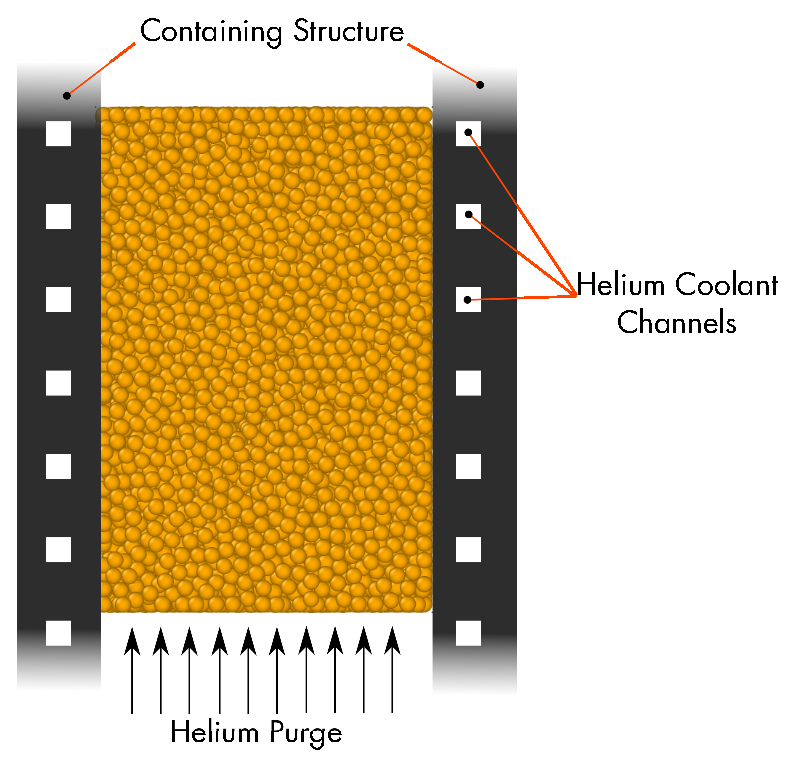
\includegraphics[width=\singleimagewidth]{chapters/figures/solid_breeder_sketch} 
	\caption{Sketch of a typical unit of a pebble bed tritium breeding zone. The pebble bed is cooled with contact to the containing structure.}
	\label{fig:solid-breeder-sketch}
\end{figure}

The breeder blanket is a critical piece of engineering technology upon which the success of a fusion power plant largely rests. The successful operation of a breeder will see the device capture the neutrons ejected from the fusion reaction to generate fuel for future reactions, act as shield to other sensitive equipment and personnel, and convert energy into extractable heat for electricity production. Figure~\ref{fig:demo} shows an example sketch of a demonstration (DEMO) fusion reactor and the relative location of the breeder blanket modules as they face the plasma in the torus of the tokamak. 

From the inception of the solid breeder concept in 1975 by Abdou\etal\cite{Abdou1975c}, designs have evolved significantly in response to requirements of operation in the harsh fusion environment. Currently, the reference solid breeder design incorporates packed beds of ceramic pebbles (spherical particles) that are filled into containment structures of volumes optimized for thermophysical and tritium responses. 

The pebble bed form has ultimately become the design of choice based on many of its attractive features. Many requirements of a solid breeder `material' (the volume of a pebble bed is often considered as a single fictitious material) are satisfied by the ceramic pebble bed. The small pebbles provide a sufficient surface-area to volume ratio; have good and customizable (via polydispersity) open-porosity to allow the helium purge gas to wind through and pick up any generated tritium from the solid; and the small size of the pebbles prevent any large thermal gradients from emerging across any single solid material object -- thus increasing the mechanical survivability of the ceramic. 

The representative pebble bed, as sketched in Fig.~\ref{fig:solid-breeder-sketch}, is shown to be contained by a low-activation steel which serves as both mechanical and thermal boundaries for the ensemble. The breeding blanket will experience high volumetric heating (resulting from secondary $\gamma$ rays and the kinetic energy of neutrons that are carrying away approximately 80\% of the fusion reaction) and temperatures will be allowed to increase to approximately 900~\celsius. The heat is conducted via inter-particle contacts between pebbles, contact with the structural material, and convection to the purge gas then transported to the structural material. A high pressure (approximately 8 MPa) helium coolant is then run through the structure. The coolant will heat to approximately 500~\celsius~before exiting the blanket, maintaining the steel below structural temperature limits. The heat carried away by the coolant ultimately works its way into an electricity-producing cycle. 

As the neutrons bombard the lithiated ceramic, tritium is produced internal to the pebbles. Tritium that transmutes from the lithium inside the pebble will diffuse slowly through the bulk until reaching a grain boundary. Tritium moves relatively quickly along the grain boundary until reaching a surface of open porosity where it may desorb into the passing purge gas.\cite{Federici1990} The low-pressure, low-speed purge gas is pumped through the pebble bed to extract the tritium generated and transport it out of the blanket for processing. 

The dual role of the breeding blanket to generate heat and tritium forces a specific operational temperature window for the ceramic pebble beds. The low end of the temperature window is governed by a minimum temperature for acceptable release rates of tritium from the ceramic to the purge gas; the value is generally set around 300~\celsius. Based on the current understanding of tritium release from the pebble, as grains grow during sintering of the ceramics the tritium release rate is expected to decrease beyond acceptable limits. Thus the upper limit of the temperature window is chosen to avoid sintering of the lithiated ceramic, giving the approximately 900~\celsius~limit mentioned previously. 

\begin{figure}
        \centering
        \begin{subfigure}[b]{\doubleimagewidth}
                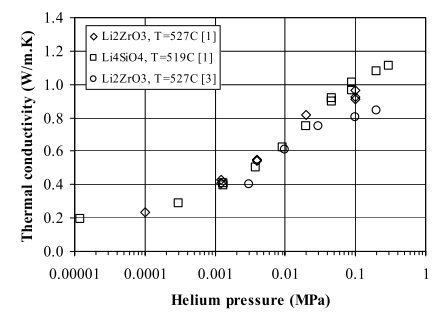
\includegraphics[width=\textwidth]{chapters/figures/keff-pressure}
                \caption{Effective conductivity of ceramic pebble beds is dependent on the pressure of the interstitial gas, a minimum of about $\keff = 1$~W/m-K in vacuum.}
                \label{fig:keff-pressure}
        \end{subfigure}%
        
          %add desired spacing between images, e. g. ~, \quad, \qquad, \hfill etc.
          %(or a blank line to force the subfigure onto a new line)
        \begin{subfigure}[b]{\doubleimagewidth 	}
                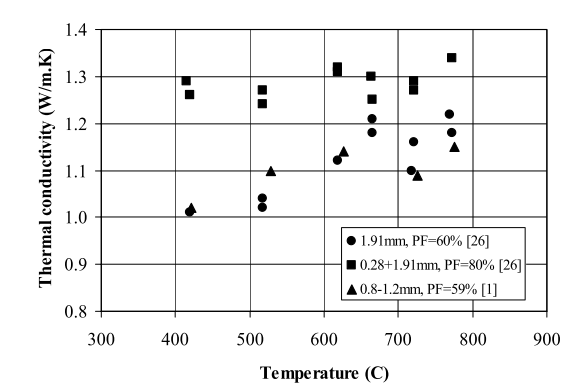
\includegraphics[width=\textwidth]{chapters/figures/lit-keff-exp}
                \caption{The effective conductivity of pebble beds is weakly dependent on external mechanical pressure and is always approximately $\keff = 1$~W/m-K in helium.}
                \label{fig:keff-lit}
        \end{subfigure}
        \caption{Effective conductivity of lithium ceramics. Results from Ref.~\cite{Abou-Sena2005}}\label{fig:keff}
\end{figure}

Many experiments have been run to measure the effective thermal conductivity of a volume of ceramic pebbles. In Figs.~\ref{fig:keff}, the effective conductivity is seen to be strongly affected by the interstitial gas but weakly affected by the mechanical loads on the bed. The main conclusions to bear in mind from Fig.~\ref{fig:keff} are that: 1) the interstitial gas is an important transporter of heat in the bed and 2) the effective thermal conductivity of the pebble bed is low and will limit the size of the ceramic pebble bed volume to satisfy the temperature window mentioned above.

% The size of breeder region is limited by the operational temperature window that must be held in spite of the the poor effective conductivity of packed beds of ceramic pebbles. The conductivity is experimentally shown to be a weak function of external pressure but can generally no greater than about \si{1 W/{mK}} -- for well-packed beds. Because the effective conductivity and packed bed-wall interface conductance is predominately a contact conduction, disruptions to the packing structure will have considerable impact on the heat transfer of the packed bed.

As nuclear energy is deposited into the poorly-conductive ceramic breeder material and the temperature climbs well above the containing structure, the pebbles will each individually begin to grow from thermal expansion. The containing structure will confine the thermal expansion of the lithium ceramic and therefore lead to large mechanical stresses at the points of contact of the individual pebbles in the packed bed. As a ceramic material, the pebbles are prone to brittle failure when the contact forces grow large. But the ceramic pebble beds must be able to survive the high temperature, high stress, and irradiated environment while providing a reliable amount of tritium to the fuel processing equipment.




 % the fusion reaction deposits   The nuclear heat generated in the pebble bed solid breeder will heat the ceramic pebbles to maximum temperatures of approximately 900~\celsius. The heat of the pebbles is transported through them via conduction through inter-particle contacts, conduction through the purge gas into neighboring particles, and ultimately through contact with the containing structure. The box structure surrounding the solid breeder will have high pressure (\si{8~MPa} in many current designs) 


\section{Motivation}\label{sec:motivation}

\begin{figure}[ht]
	\centering
	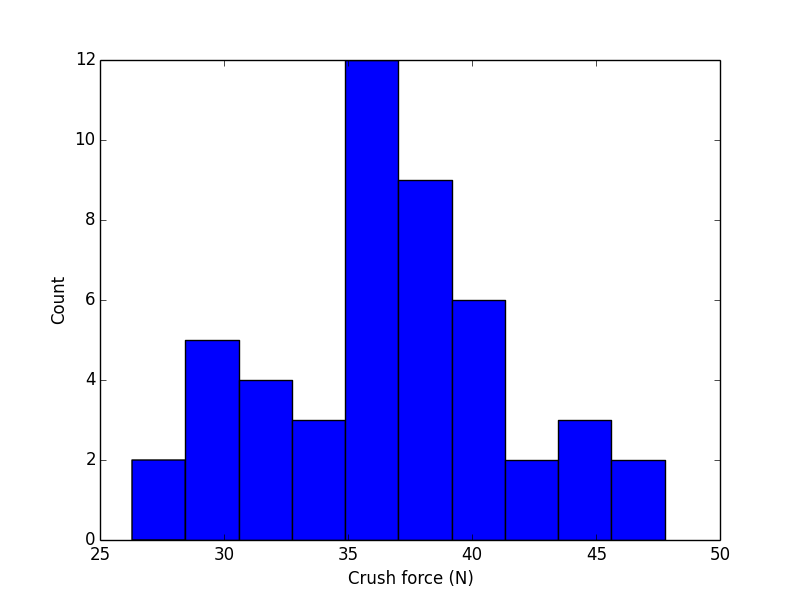
\includegraphics[width=\singleimagewidth]{chapters/figures/fmax} 
	\caption{Crush load distribution for a batch of $d_p = 1$~mm \lit pebbles.}
	\label{fig:fmax}
\end{figure}


Experiments on individual particles betray the brittle nature of ceramic pebbles and their propensity to break at relatively low individual contact forces. An example histogram of the crush loads of a batch of 1~mm \lit pebbles, as measured in our lab, is shown in Fig.~\ref{fig:fmax}. For these particular pebbles, the average crush load was less than 40 N. For some \lis pebbles, the average crush load is measured as low as 10 N. The relatively low force required to crush, coupled with the strong macroscopic loads predicted by the FEM models, brings into question the survivability of the pebbles and packing of the solid breeder.

If individual pebbles in the packed bed ensemble begin to crush, it may result in a number of negative effects on the bed. First, from Fig.~\ref{fig:keff-pressure}, we can see that a significant amount of heat (roughly 20\%) is transported through the bed purely via contact conductance between pebbles. In response to damaged pebbles, the bed will resettle from the imbalance of inter-particle and gravity forces. Any disruption in the contact network will have an impact on the heat paths internally and at the bed-wall interface. A bed with damaged pebbles could have significantly different effective thermophysical properties than those predicted for the original bed, potentially increasing the overall temperature of the bed past the acceptable temperature windows described in the previous section. Furthermore, the neutron absorption/shielding function of the solid breeder is dependent on an assumption of homogeneous distributions of pebbles in the breeding unit volume. Broken pebble fragments will settle, in time, in the direction of gravity and accumulate at the floor of the pebble bed, concurrently the entire bed may be resettling and a physical gap at the top of the pebble bed can form. This would result in undesirable quantities of neutrons streaming past the solid breeder volume. 

As the thermophysical properties evolve, global or local bed temperatures change and ultimately the tritium release characteristics of the bed deviate from any prediction one may have had from the initial packing of the ceramic pebble bed. The ceramic solid breeder must continue operating despite the harsh effects of existing in the fusion reactor. And it must continue operating without being replaced or actively maintained. Its important that the solid breeder not simply survive the thermal and mechanical demands of the reactor environment but continue to release predictable and acceptable amounts of tritium. 

In light of the short discussion above, it is apparent that a thorough study of pebble damage, including the loads on the pebble bed that will lead to broken pebbles as well as the pebble bed's thermophysical responses to broken pebbles, is critically needed for solid breeder design. Unfortunately, pebble bed experiments are inadequate for this need. The majority of measurements are only available for macroscopic properties (\textit{e.g.} uniaxial compression tests for stress-strain responses) or give only maximum measurements of individual pebble responses (\text{e.g.} pressure sensitive layers giving pebble pressures on a wall). The inability of physical experiments to reliably look into the transient inner structure of the pebble bed has driven past solid breeder researchers to employ pebble-scale models. Increasingly reliable and accurate models are crucial in the design of operational solid breeder blanket technologies. In this dissertation, I attempt to advance the field of solid breeder pebble-scale modeling with the introduction of new techniques and tools to incorporate the many facets of pebble damage in a solid breeder.

Briefly, I must consider why one would employ pebble-scale models versus those that are bed-scale. Afterall, the volume of a pebble in a tritium breeder is on the scale of 10$^{-9}$~m$^3$ while the typical container volume can be on the order of 10$^{-2}$~m$^3$\cite{Cho2008}.  Thus a single breeder volume will house upwards of $N = 10^7$ pebbles. Statistically then, it is reasonable to assume that continuum theory is applicable to the ensemble of pebbles. This assumption is the basis of development of finite element method (FEM) models for the breeder pebble beds. Constitutive equations are developed from experimental measurements of the macroscopic behavior of pebble beds which are fed into FEM models. The continuum assumption allows modeling the thermomechanical interaction of the entire pebble bed with the containing structure and coolant. The FEM models have been able to predict thermo-mechanical behavior with reasonable accuracy of some lab-scale experimental mock-ups of breeding units (A more thorough summary of the state of solid breeder modeling is given in \cref{sec:modeling-state}).\cite{DiMaio20081287,Zaccari20081282,Gan:2009vn} A notable result indicated by all the different FEM models is the indication that strong mechanical loads will arise throughout the pebble bed -- which will lead to many histrionic effects. But it is these very histrionic effects that FEM is, at present, incapable of modeling: pebble damage, resettling, and gap formation. The focus of this dissertation is on the histrionic effect of individual damaged pebbles and the morphological changes they induce in the pebble bed writ large. Thus I am compelled to consider the models at the scale of the individual pebbles.

\section{Scope of the Work}\label{sec:intro-scope-of-work}

In our group we identify the need to predict pebble damage in an ensemble, understand of the evolution of pebble bed morphology due to pebble damage, and analyze the impact of morphological changes on thermophysical and thermomechanical properties. To satisfy these needs, the work of this dissertation is to develop tools for modeling pebble interactions, predict pebble crushing based on the interactions, and monitor the macroscopic changes to temperatures in the bed in response to damaged pebbles. On the path of pebble-scale modeling development, I will:
\begin{enumerate}
	\item validate the Hertzian assumption for ceramic pebble interactions with single experiments on crushing pebbles,
	\item derive a criteria for pebble crushing in our numeric ensemble based on single pebble experiments,
	\item assess the impact of fragment size on packing resettling and other morphological features,
	\item calculate the evolving force network and its influence on the heat transport in the pebble bed.
\end{enumerate}

After implementing a sophisticated pebble-scale modeling tool, I will show the limitations of the micro-mechanical model when it comes to simulating the heat transfer of a ceramic pebble bed with a creeping helium purge gas. Thus I also implement some efficient bed-scale models of thermo-fluid flow coupled to/integrated with particle-scale mechanics. The steps toward achieving these models includes:
\begin{enumerate}
	\item adapting and employing two numerical schemes to study packed bed energy transfer with interstitial gas,
	\item analyze the reduction in $\keff$ due to broken pebbles,
	\item study the lumped-capacitance assumption (innate to the particle-scale modeling approach) in a packed bed with high Biot number with nuclear heating.
	\item address the overall impact of the helium purge gas on the thermal transport in a bed with evolving morphology,
\end{enumerate}

Finally, when the particle-scale model predicting and simulating pebble damage is coupled to thermo-fluid models of the helium purge through packed beds, I will use the numerical tools to judge the consequences of pebble damage on two ITER-relevant configurations of breeder volumes, applicable as guidance to solid breeder designers.



% The objective of this dissertation is to develop numerical models of ceramic pebble beds, based on first principles and experimental observations, to simulate the hysteritic evolution of pebble bed morphology and predict the subsequent changes to heat transport characteristics after thermally-induced damage to pebbles. The numerical tools are constructed in the following progression: 1. Transient DEM code of inter-particle interactions is employed to simulate packed bed restructuring in the wake of crushed pebbles in the ensemble -- and the effective thermal conductivity following the restructuring, 2. Transient, volume-averaged equations of Navier-Stokes and energy of the helium purge gas are coupled to the DEM model of pebbles to simulate conjugate heat transfer and the interstitial fluid influence on thermophysical properties after crushing events, 3) Complete simulations of the tortuous path of helium purge gas with lattice-Boltzmann models (based on the packing structure determined in DEM simulations) to expose flattened temperature profiles due to laminar mixing in the pebble bed. 

In summary, understanding the evolution of pebble bed morphology and its impact on thermophysical properties is critical for solid breeder designers. The understanding allows for temperature control of breeder pebble beds over the operational lifetime of the blanket which is crucial to the function of the solid breeder for tritium and energy generation. The tools I develop in the course of this dissertation are a necessary step toward realization of this understanding. 

One last note: there are other long-term effects expected in the materials experiencing prolonged exposure to cycling irradiation, heat, and stress that have not been discussed here. These loads can lead to thermal ratcheting, irradiation swelling, sintering, or thermally-induced creep which also lead to evolutions in thermophysical properties -- even in the absence of cracked pebbles. These phenomena need to be addressed in time but are, however, beyond the scope of this dissertation. 
% we aim to provide designers of packed beds with tools to understand how packing states may evolve from time-dependent phenomena (e.g. sintering, creep, pebble cracking, etc.). These phenomena may, for instance: decrease the effective thermal conductivity which will raise bed temperatures beyond initial predictions, produce isolated pebbles which will sinter and potentially decrease tritium release rates, or even form gaps between pebble beds and containing structures leading to divergence from properties of the initial packing of the bed.

% The objective of this work fits into the broader mission of our research group in the UCLA Fusion Science and Technology Center to develop and apply complete numerical models of ceramic pebble bed solid breeder modules. Any complete numerical model for a pebble bed would require the interaction of many sub-models or sub-functions operating at disparate scales. To demonstrate, a possible top-level algorithm could proceed in the following way: To begin, one must have knowledge of the interaction of the pebble bed with the containing structure as they exist in a fusion environment. The interactions are generally analyzed via the finite element method to find internal stresses and temperature fields of the entirety of the pebble bed and surrounding container. After the internal fields are mapped into the bed, one would use the discrete element method (DEM) to interpret the macroscopic stress fields into the inter-particle forces. With the inter-particle forces and total absorbed thermal energy calculated, a prediction of the initiation and evolution of morphological changes (i.e. crushed pebbles, sintering, creep, etc.) to each computational volume. Following this, DEM would calculate new effective properties as a result of the morphological changes to the pebble bed region. Finally, the updated bed properties would feed back into the FEM formulation to update calculations in the macroscopic stress fields. While a suite of integrated numerical tools that follows this example algorithm is the ultimate goal of our group, the work of this dissertation is focused entirely on the development of pebble-scale simulations that are predominately in the realm of the discrete element method.

% In the following subs-sections, we briefly outline the studies fitting into the scope of this dissertation. 

% \subsection*{Discrete Element Method Study on the Evolution of thermo-mechanics of a Pebble Bed Experiencing Pebble Damage}
% In the first study of \cref{sec:dem-studies}, we analyze the effective thermal conductivity of a pebble bed assuming different fractions of pebbles in the ensemble are completely crushed. The focus of this study is to 1) determine the extent of change, in aggregate, to ensemble properties due to individual pebble crushing, 2) relate the changes in effective conductivity to quantifiable pebble-scale properties (e.g. contact force, coordination number, etc.), 3) use the results to create guidelines for designers to anticipate acceptable limits of pebble loss from a thermal management point of view. For the DEM tools used in this study, the only mode of heat transfer considered is conduction between the solid particles. 


% \subsection*{Coupling DEM Models of Ceramic Breeder Pebble Beds to Thermofluid Models of Helium Purge Gas Using Volume-averaged CFD}
% In a fusion breeder, the helium purge gas winding through the interstitial gaps of the pebbles has a substantial contribution to overall heat transfer.\cite{Reimann:2002mi,Abou-Sena2005} The model of \cref{sec:dem-studies} is improved to include the flowing interstitial gas. In \cref{sec:cfd-dem-studies}, we continue to employ our DEM tools to provide particle-scale information such as contact force, but couple the pebbles to a volume-averaged computational fluid dynamics (CFD) code for the conjugate heat transfer simulation. The coupled CFD-DEM model is used to again simulate the heat transfer in packed beds of ceramic spheres that experience pebble crushing -- but now with a focus on highlighting the impact of a flowing interstitial helium purge gas when pebbles are crushed.


% \subsection*{Lattice-Boltzmann Method Integrating DEM Packing Structures to Study Laminar Mixing}
% The models to account for helium purge gas employed in the studies of \cref{sec:cfd-dem-studies,sec:applied-studies} assume effective drag or heat transfer coefficients for pebbles in a computational volume and then include the pebble influence through effective source/sink terms in the momentum and energy equations. The volume-averaged approach allows for simpler meshing of the fluid volume while still retaining much of the physical realism of the system. Complete models of the conjugate heat transfer of both the fluid moving through the tortuous interstitial gaps pebble beds pressing each other with small contact areas are intractable with current computational hardware and finite-element modeling techniques. To overcome deficiencies in computational power, in \cref{sec:modeling-lbm}, we apply a relatively new technique wherein a lattice-Boltzmann algorithm solves for complete flow fields and conjugate heat transfer of helium winding through a packed bed. The lattice-Boltzmann method (LBM) is a non-traditional fluid simulation technique that allows us to resolve pebble/pore-scale momentum and energy transfer. The LBM approach is applied to the same pebble beds analyzed in \cref{sec:cfd-dem-studies} to provide comparison between the two modeling techniques. Furthermore the LBM model, accounting for the complex helium purge gas pathways, provides more insight to the influence of helium on the heat transfer in the heat transfer of packed beds.





% \subsection*{Modeling Tools to Study Coolant Designs of ITER Solid Breeder Module Volumes}
% In the study of \cref{sec:applied-studies}, we apply our coupled helium-pebble computational tools to the analysis of ITER-relevant solid breeder geometries. In this study we consider the combined effects of pebble crushing, packing restructuring due to both gravity and the unbalanced force network in the pebble bed, and convection from helium purge gas on temperature profiles in solid breeders for different breeding configurations. Heat transfer out of the pebble bed relies on maintaining good pebble-pebble and pebble-wall contact. However, physical contact is interrupted to different degrees when a pebble bed responds to various amounts of individual crushed pebbles. Furthermore, the restructuring of the pebble bed after a pebble crushing event is, in part, dependent on gravity forces acting upon each pebble in the ensemble. We investigate two representative pebble bed configurations where heat is removed from the bed via inter-particle conduction, convection of purge gas, and contact between the pebble bed and its container. In the first, the coolant containing structural walls (heat transfer walls) are oriented parallel to the gravity vector. In the second configuration, the heat transfer walls are perpendicular to the direction of gravity. To simulate a crushed pebble, we replace the pebble with many smaller, non-cohesive elements while maintaining mass-conservation between the original solid pebble and crushed fragments. The fragments are then free to resettle into interstitial gaps and the rest of the bed resettles as determined by forces from gravity, contact of neighboring particles, and even the small influence of the moving purge gas. The thermo-fluid interaction with the helium purge gas will be included with volume-averaged Navier-Stokes and energy equations. The representative solid breeder volumes will be compared with respect to their temperature peaks and profiles and how those temperatures vary as a function of the percentage of crushed pebbles in the ensemble. The results can be used to optimize solid breeder pebble bed designs through the choice of breeding zone orientation relative to the gravity vector.



% \chapter{Dissertation Outline}
% The path toward the modeling efforts outlined for the scope of this work is not a clear, straight line. To accomplish the goals set forth -- attempting to discuss them in the most clear and accurate way possible -- this dissertation is broken up into five major parts following their logical partitions. This section, Part I, provides the introduction and motivation behind the work. In Part II, (containing Chapters: \cref{sec:hertz-theory,sec:modeling-state,sec:survey-packed-beds}) we survey the state of the art in analysis of ceramic pebble beds, contact mechanics, and modeling thermal and mechanical interactions of particles in packed beds and fluids moving interstitially.  In Part III, (containing Chapters: \cref{sec:modeling-dem,sec:modeling-cfd-dem,sec:modeling-lbm}) we outline the numerical methodology and development of modeling tools we shall use in the study and analysis of pebble beds and their evolving morphology due to external loads. We compartmentalize the numerical tools into three parts, namely: the discrete element method (DEM), coupled computational fluid dynamics and the discrete element method (CFD-DEM), and a lattice-Boltzmann method (LBM) we integrate with DEM. The development of the tools is assisted with theoretically- and experimentally-based studies on individual pebbles in an ensemble. The newly developed enhancements to the numerical tools are studied before their inclusion in the toolkits. We work through the results of the promised studies in Part IV (\cref{sec:cfd-dem-studies,sec:dem-studies,sec:lbm-studies,sec:applied-studies}). Finally, in Part V, we discuss the next steps to be taken that we identify as critical next steps -- but beyond the scope of this dissertation -- for the modeling tools. In addition, other research avenues that have been opened by the tools introduced and their potential impact are discussed here.

% Literature Review
\chapter{Status of Ceramic Breeder Modeling and Analysis}
A common problem plaguing those who study packed beds is the multi-scale of physics dictating the behavior of the packed bed. In the realm of engineering continuum mechanics, packed beds cannot be adequetly described as a solid or liquid (or obviously gas) alone. Under compression, a packed bed responds like a solid with non-linear elasticity and a plasticity that is history-dependent. The packed bed can obviously not support any tensile pressure and will often behave like a liquid as it may fill in voids under just the force of gravity. Experiments on packed beds provide effective material properties that are often specific to the material, packing fraction, moisture content, or level of polydispersity.

In packed beds of ceramics for tritium breeding, phenomenological models have been developed based on the controlled environment of laboratory experiments. The models provide reliable information on the initial states of breeder volumes in the fusion reactor environment and allow reasonable design predictions of the thermomechanics of the breeding blanket. Unfortunately, a certain measurable quantity in an experiment may arise due to vastly different pebble-scale physics. Furthermore, it is unavoidable that other morphological changes of the pebble bed may arise due to individual pebble cracking, inter-particle creep, or inter-particle sintering. Designers of solid breeder blankets must have predictive capabilities for the initiation of morphological changes in the packed bed as well as how those changes impact the thermophysics of the bed.

The solid breeder in many current designs feature sub-module units of packed beds. From the point of view of pebble bed thermomechanical properties, this has the advantage of producing units individually that can be tested and qualified to desired packing states (and therefore thermomechanics) during the design phase. 



The thermophysical and thermomechanical properties of pebble beds have been studied extensively [cite many of the experimental papers]. From experimental measurements, and the assumption that a pebble bed can be treated as a continuous media, researchers have developed phenomonological formulas relating properties of pebble bed to other, measurable, macroscopic properties [cite many of the modeling papers]. For instance, an effective thermal conductivity can be given for the packed bed given a certain gas and stress on the bed. These effective material properties are useful for the design and qualification of tritium breeding modules. But it must be understood that the material properties of a pebble bed are a function of their history and will evolve in time as the morphological features of the pebble bed likewise evolve in time. Therefore there is a need to predict the morphological changes to the pebble bed and the subsequent impact on the bed's thermophysical properties so that solid breeder designers may have reliable temperature control of the pebble bed over the duration of the use of the breeder in the reactor. 

^^ above is copied from old sections but seem more appropriate here
%~~~~~~~~~~~~~~~~~~~~~~~~~~~~~~~~~~~~~~~~~~~~~~~~~~~~~~~~~~~~~
Ceramic breeders, by their nature, are brittle and prone to cracking under external mechanical loadings. These breeders, in the form of packed beds of pebbles, are loaded into a box-like structure for tritium fuel production in a fusion reactor. When subjected to nuclear heating in a reactor, a strong mechanical loading arises from the differential thermal expansion between breeder pebbles and their containing structure. Research efforts have therefore been aimed at developing a thorough understanding and characterization of the ceramic breeder pebble bed thermomechanics. Such an understanding is essential to providing confidence in the performance and lifetime of a ceramic breeder blanket design. In particular, a significant effort of the pebble bed thermomechanics study is on the development of modeling simulation tools. 

Reimann, et al. have conducted an extensive experimental study of the stress-strain relations of the ceramic breeder pebble beds using an oedometric test apparatus \cite{Piazza2002811,Reimann:2002kl,Reimann:2003qc,Reimann:2002mi,Reimann:2001il}. The most significant macroscopic experimental phenomena witnessed in the pebble bed are an irreversible plastic strain when the load is removed, a non-linear elasticity, a pressure-dependent plasticity, and a volumetric creep.  A particularly noticeable feature, clearly demonstrated in Fig.~\ref{fig:mti}, is the reduced amount of irreversible strain when subjected to additional loading cycles after the first unloading. This may suggest the existence of a semi-equilibrium packing state in the pebble bed which can be reached after applying a pre-load to account for the large strain in the first cycle of a pebble bed. This semi-equilibrium packing state is a feature which may be advantageous for use in a fusion reactor. 

To study the temperature effect in Reimann's studies, the bed is freely heated to the desired working temperature before the pressure load is applied. Under the same loading condition, the bed behaves much softer at higher temperatures. The bed stiffens as the pressure increases. An illustration of this phenomenon is presented in Fig.~\ref{fig:UCT} for a lithium orthosilicate pebble bed between $50-850^\circ$C. At higher temperatures (such as $> 650^\circ$C), a creep-like behavior becomes apparent. The creep behavior allows the pebble bed to relax and sustain higher stresses, however one needs to avoid sintering. The data was used to correlate creep rate as a function of temperature, stress, and time for both lithium orthosilicate, lithium metatitanate, and beryllium pebble beds \cite{Buhler:2002qf,Reimann:2001il,Reimann:2005qa}.


\begin{figure}[t!]
\begin{center}
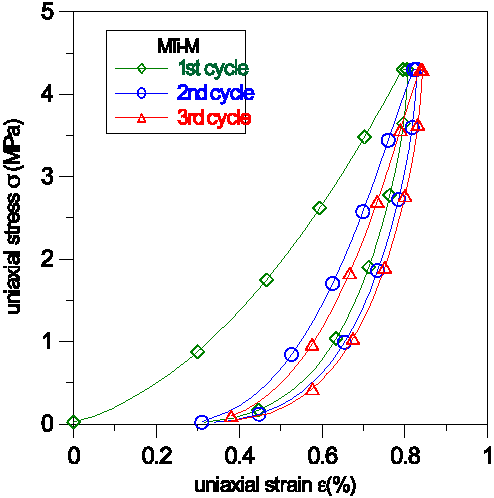
\includegraphics[width=0.4\textwidth]{chapters/figures/Fig-1}
\caption{Example of uniaxial compression testing results for lithium metatitanate pebble bed \cite{vanderlaan2011}.}
\label{fig:mti}
\end{center}
\end{figure}

\begin{figure}[t!]
\begin{center}
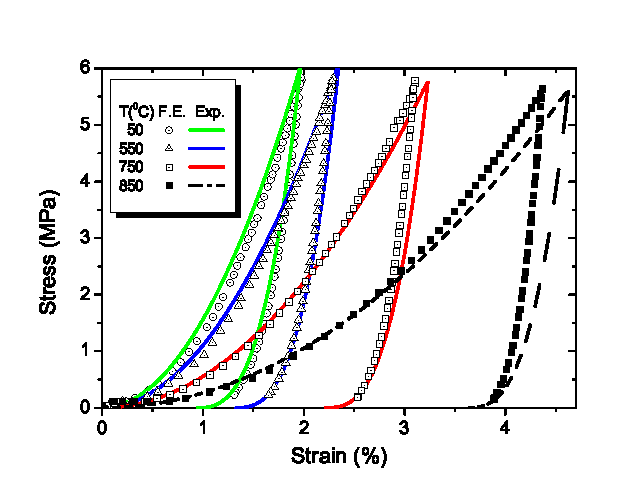
\includegraphics[width=0.5\textwidth]{chapters/figures/Fig-2}
\caption{Example of uniaxial compression testing results compared with predictions from material constitutive equations for lithium orthosilicate pebble beds at different temperatures \cite{Gan:2008kx}.}
\label{fig:UCT}
\end{center}
\end{figure}

Phenomenological models, derived from the volumes of collected data, have been proposed to describe the aforementioned mechanical behavior of the pebble beds with a conventional continuum-based approach. The continuum approach allows treatment of the pebble beds with standard finite element modeling (FEM). To employ FEM, mathematical models written in terms of average quantities and containing effective parameters are used. These models deduce a set of constitutive equations to be implemented in the framework of a finite element code.  There are two major variants of phenomenological modeling approaches developed among institutions, including: (1) A non-linear elastic model and a modified Drucker-Prager-Cap theory for plastic strain \cite{Gan2007189,fokkens2003}; and (2) A hyperporous non-linear elastic model and a Gurson model for plastic model \cite{DellOrco:2007hc,DellOrco:2010zr,DiMaio20081287}. The readers are referred to the additional efforts used in a third method\cite{fokkens2003} which employed two different elasticity laws for the loading and unloading branches but will not be discussed here. Alongside the development of the modeling techniques, several large scale pebble bed thermomechanics experiments were conducted in parallel. These experiments were intended to reveal the underlined thermo-mechanical characteristics of ceramic breeder pebble beds, and provide data for benchmarking the developed models.   The validation statuses as well as the features of the models are briefly described in the following section. 

Another modeling strategy is to model the pebble bed as a system of distinct interacting bodies that are subject to forces and resulting motions. This modeling approach called discrete element modeling (DEM) considers the mechanical interaction between pebbles and numerically solves the associated equations of motion \cite{An20072233,An20071393,Gan:2010uq,Gan20101782}. The DEM approach has recently received increased attention and the progress will be summarized to follow.

The review of the current status of development on the ceramic breeder pebble bed thermomechanics is organized as follows. In Section 2, current continuum modeling approaches and constitutive models for mechanical and thermal interactions are presented. In Section 3, a review of recent advancements on DEM is presented. A brief discussion on recently-initiated benchmarking efforts, in-pile experimental results, and other experimental observations relevant to pebble bed thermomechanics are given in Section 4. A proposed framework and a few conclusions on the outlook are drawn in Section 5. 


%%%%%%%%%%%%%%%%%%%%%%%%%%%%%%%%%%%%%%%%%%%%%%%%%%%%%%%%%%%%%%%%%%%%%%%%%%%%%%%%%%%%%%%%%%%%%%%%%%%%%%%%%%%%%%%%%%%%%%%%%%%%%%%%%%%%%%%%%%%%%%%%%%%%%%%%%%%%%%%%%%%%%%%%%%%%%%%%%%%%%%%%%%%%%%%%%%%%%%%%%%%%%%%%%%%%%%%%%%%%%%%%%%%%%%%%%%%%%%%%%%%%%%%


\section{Status of Continuum Modeling Approaches}
\subsection{Mechanical constitutive equations}
Continuum models focus on predicting global behavior, including volumetric strain and stress and the impact on the effective thermal conductivity, etc. Two institutions in Europe have spearheaded modeling efforts. One being Karlsruhe Institute of Technology, formerly FZK and referred to as such throughout this paper, and the other being ENEA-Brasimone with the Department of Nuclear Engineering at the University of Palermo, referred to as DIN throughout this paper. These two institutions have published a great deal of detail in regards to the specific details of their modeling techniques and the reader is referred to these publications for the fine points of the models \cite{DellOrco:2007hc,DellOrco:2010zr,DiMaio20101234,Gan2007189}. The discussion here calls attention to differences between models and attempts to serve as a reference basis for future modeling efforts.

The models from FZK and DIN share a common treatment of the mechanical interaction between the pebble beds with structural walls. In models from the two institutes, interfacial contact and friction forces are taken into account by application of the Coulomb friction law. This frictional contact law can be simply implemented in finite element code without considerable computation effort.

\subsubsection{FZK mechanical model}
In the FZK approach, the corresponding phenomenological constitutive models were developed based on the soil mechanics models implemented in the finite element code ABAQUS. This includes a non-linear elasticity model, which was originally developed for powder die compaction; a plastic strain model via a modified Drucker-Prager-Cap model, which was originally developed for soil mechanics; time-dependence via a consolidation creep law; and global thermal-mechanical coupling from material parameters.

The Drucker-Prager-Cap model captures the plasticity of the pebble beds and predicts the yielding and hardening behavior. A feature of the classic Druger-Prager-Cap model, as implemented in ABAQUS, is the ability to describe the plastic behavior of pebble beds under hydrostatic compression; a feature which is not present in classical metal plasticity models. However, researchers at FZK recognized that for materials with large creep strain amplitudes (e.g. beryllium pebble beds), hardening laws defined by default in ABAQUS were insufficient. Therefore, unique hardening laws were developed and implemented in place of the standard equations referenced in ABAQUS. An advantage gained from the redefined hardening laws is their capture of the creep behavior witnessed in pebble beds at high temperatures. The disadvantage of the Drucker-Prager-Cap model is the computational resources necessary for convergence of solutions. This has so far limited the FZK model to spatially two-dimensional simulations.

The main distinguishing feature unique to the continuum model developed in FZK is in their treatment of the material parameters that feed into the models described above. In particular, the hardening law in the model is manipulated to accommodate direct fitting to the oedometric tests. Unlike other continuum models, which require a trial-and-error method of optimizing numeric elasto-plastic parameters, the FZK model can be directly and clearly linked to experimental data. In this way, the model may be most adept at predicting behavior of a pebble beds where stress and temperature fields are very different from the controlled experiments which produced the constitutive relationships \cite{Gan2007189,Gan:2009vn,Gan:2010lh,Gan:2010kc}.

\subsubsection{DIN mechanical model}
The mechanical model established in the DIN model similarly assumes a non-linear elasticity model and a plasticity model. The non-linear elastic model assumes that during the reversible straining of a pebble bed, its effective logarithmic bulk modulus depends on the equivalent pressure according to a hypothesized power law. From this assumption as the foundation, DIN proceeds through a semi-theoretical derivation to relate the bed deformation modulus to the equivalent pressure; and stress state to volumetric strain. Included in the derivation are a number of effective parameter values. Values of all material parameters are chosen on an iterative trial-and-error basis until the model agreed well with the non-linear, elastic curves seen in oedometric experiments.

Attempting to resolve large computing time required when using the Drucker-Prager-Cap model for plastic deformation, DIN instead used a Gurson model. The Gurson model was originally developed for the analysis of pressure-dependent plastic behavior of mildly voided materials. The Gurson model postulates that the pebble bed behavior can be modeled as a continuous matrix in which stochastically-distributed voids are contained. In the Gurson model, compaction-related plastic deformation of the bed can to be reproduced. For material parameters in the Gurson model, again an iterative procedure was used until the model reproduced the results of relevant experimental tests. Lastly, in the consideration of the effective hardening law in pebble beds, a fifth order polynomial function was hypothesized. It should be noted that in the model's current form, it is incapable of directly capturing the creep behavior of pebble beds. However, the model was designed such that a future creep law could readily be implemented \cite{DellOrco:2007hc,DellOrco:2010zr,DiMaio20101234}.

The main advantage of the approach taken by DIN in their model is apparent when considering computational demand. DIN is currently able to model three-dimensional experiments with modest computer time. The most apparent drawback is the ad-hoc procedure of determining effective parameters used in the model. Without a direct link to experimental data, the applicability of the chosen effective parameters at predicting behavior beyond the range of the experimental conditions is unknown.

\subsection{Mechanics and heat transfer coupling}
Maintaining the breeder temperature within its temperature window is crucial for predictable performance and lifetime of the breeder unit. Proper temperature analysis requires careful characterization of thermal properties of the pebble beds. 

The pebble-bed experiments demonstrated that the effective thermal conductivity depends on the volumetric compressive strain; changes in thermal conductivity occurred between compacted and un-compacted systems. These measured phenomena indicate that thermo-mechanical modeling must also consider full, non-linear coupling between thermal and mechanical analysis.

The thermal models of the two institutions are fundamentally similar. The form of thermal model used by FZK follows from the experimental work carried out by J. Reimann from FZK in which empirical equations have been reported where the temperature and volumetric inelastic strain-dependence is incorporated into the bulk thermal conductivity. The thermal conductivity for a lithiated ceramic pebble bed over a specified range of temperature is reported in Ref.~\cite{Gan2007189} as:
\begin{align}\label{eq:fzkK}
k \left(W/m \cdot K \right)& = 1.81+0.0012  \,T - 5 \times 10^{ - 7} \,T^2 + \nonumber\\
&+ \big(9.03-1.386\times10^{-3} \,T-7.6\times10^{-6}\, T^2 + \nonumber\\
&+ 2.1\times10^{-9} \,T^3\big)\epsilon
\end{align}
where $T$ and $\epsilon$ are the local temperature and strain, respectively. The formula for thermal conductivity owes its functional form to the widely used Schlunder, Zehner, and Bauer (SZB) model. The coefficients in Eq.~\eqref{eq:fzkK} are empirically derived from experiments. The FZK model has  linked its constitutive equations directly to experimental data. 

In the DIN thermal model, the effective thermal conductivity has a quasi-linear dependence on volumetric strain and temperature. DIN reports the equation for determining thermal conductivity in Ref.~\cite{DellOrco:2007hc}, it is:
\begin{align}\label{eq:dinK}
k\left(W/m \cdot K \right)&=\lambda_0\left(1+\gamma T+\delta \epsilon\right)
\end{align}
where T and $\epsilon$ are the local temperature and strain, respectively. The relationship of Eq.~\eqref{eq:dinK} introduces several effective parameters, $\lambda_0$, $\gamma$, and $\delta$, that are determined from iterative fits to experimental data. Values of these effective parameters have been determined thus far for beryllium and certain lithium orthosilicate pebble beds\cite{DiMaio20101234}. The thermal conductivity, being a function of both thermal and mechanical parameters endows the models with a full coupling between thermo-mechanical analyses. 

\subsubsection{Thermal interface model}
The thermal interaction at the interface between pebble bed and containment wall is represented in both models as an effective heat transfer conductance, with only slight variations between the two approaches. In the FZK model, the thermal interaction is simulated with an effective heat transfer coefficient. The heat transfer coefficient (HTC) incorporates the combined effects of radiation heat transfer, pebble-solid conduction, and solid-gas heat transfer. Furthermore, in the event of a gap formation at the interface between pebble bed and containing surface, a separate heat transfer coefficient is employed. The researchers at DIN noted that interface conductance is affected by parallel paths of heat flow: pebble-wall conduction at contact areas and gas-wall convection. DIN therefore posits that the macroscopic phenomena can be modeled as a pressure-dependent thermal gap at the interface. They therefore have a thermal interface conductance that is a function of temperature, pressure, and local volumetric strain. An iterative trial-and-error method was also used to determine the effective parameters in this term. 


%%%%%%%%%%%%%%%%%%%%%%%%%%%%%%%%%%%%%%%%%%%%%%%%%%%%%%%%%%%%%%%%%%%%%%%%%%%%%%%%%%%%%%%%%%%%%%%%%%%%%%%%%%%%%%%%%%%%%%%%%%%%%%%%%%%%%%%%%%%%%%%%%%%%%%%%%%%%%%%%%%%%%%%%%%%%%%%%%%%%%%%%%%%%%%%%%%%%%%%%%%%%%%%%%%%%%%%%%%%%%%%%%%%%%%%%%%%%%%%%%%%%%%%



\section{Discrete Element Method}
Discrete Element Method (DEM) introduced by~\cite{Cundall1979} has been shown to be a promising tool to study the behavior of granular systems through the interaction between the individual particles. DEM has been used successfully to study the micromechanical aspects of pebble bed thermo-mechanics in the past~\cite{An20072233,Gan:2010uq}. Furthermore, DEM can be used to establish a relation between the microscopic interactions and the macroscopic response of the granular assemblies. Reference \cite{An20072233} studied the pebble assemblies in rectangular and cylindrical containers bounded by a elastic walls. The effect of packing factor, geometry of the assembly on the overall stress-strain response under uni-axial compression tests (UCT) has been thoroughly investigated. \cite{Gan:2010uq} have studied similar pebble assemblies in a cubic box with periodic boundary conditions. In both the above studies, a non-linear stress-strain response and a characteristic residual strain after unloading (analogous to plastic strain in continuum systems) has been observed akin to the experimental results~\cite{Reimann:2000tw}. It has been shown that the average coordination number, average normal contact force and the maximum normal contact force in the assembly has a unique functional relation (nonlinear, linear and linear, respectively) with the hydrostatic pressure or the applied pressure independent of the packing factor~\cite{Gan:2010uq,An20071393}. These functional relations may be used as master curves for the micro-macro correspondence in the pebble bed thermo-mechanics studies. A first attempt to include the creep mechanism in DEM has been made by~\cite{An20071393} showing the experimentally observed phenomenon such as the reduction of creep strain rate over time under constant load, albeit qualitatively. Further advances in the thermo-mechanics of pebble beds using DEM are under progress at KIT and UCLA in collaboration with experiments.

Recently, the effect of the pebble size distribution on the overall thermo-mechanical behavior of the pebble assembly is studied by~\cite{Annabattula2011} considering the pebble size distribution of ceramic breeder pebbles (Orthosilicate (OSi) pebbles) with a diameter range of $0.25~\mathrm{mm}$-$0.65~\mathrm{mm}$. Figure~\ref{fig:pebble-assembly-potential-energy} shows a binary pebble assembly in a periodic box. The colors indicate stored elastic strain energy of the pebble (red: maximum and blue: zero). The assembly has a maximum pebble radius $\rmax=0.25$ mm with the pebble size ratio $\rstar=\rmin/\rmax=0.6$, relative volume fraction $\vstar=\vmax/V=0.7$ and a packing factor $\eta=0.643$. The average stress in a granular assembly can be deduced from the contact forces between individual grains.

Another aspect of interest in the study of mechanics of pebble beds is the crush behavior of individual pebbles and their impact on the over all pebble bed response. DEM is used to study the behavior of a crushable pebble assembly with the crush load data for OSi pebbles (for individual pebbles) measured at KIT for pebbles of diameter 0.5 mm. 

A probabilistic method for analyzing the crush events of individual pebbles and a procedure with the combination of DEM and experimental data to obtain crush load probability has been reported by~\cite{Gan:2010kc}. Figure~\ref{fig:cdf_pebbles} shows the cumulative distribution function as a function of the hydrostatic pressure placed on the bed. The probability analysis, derived from DEM calculations, provides quantitative report of pebble crushing as a function of a specific hydrostatic pressure. The results of this analysis exemplify the growing strength of DEM techniques for analyses connecting global pebble bed loads to individual pebbles.

However, it has been shown~\cite{Zhao2010,Zhao2011} that a criterion based on critical stored elastic energy is the most suitable criterion for describing the OSi pebble failure. Hence, the crush load data (provided by fusion materials laboratory at KIT) has been transformed into equivalent elastic strain energy showing a Weibull distribution~\cite{Zhao2010}. This critical energy (randomly generated distribution) is used as the criterion for failure of pebbles in the DEM simulations. First, the assembly is loaded up to 3\% strain in uniaxial compression and then unloaded to a stress-free state. The elastic modulus of the pebble is reduced (from initial value to a small value of 1 kPa) with increase in elastic strain energy of the pebble according to a phenomenological damage accumulation law~\cite{Annabattula2011b}. The damage state is frozen at the end of loading step and hence there will be no further damage accumulation in the unloading step. 

Figure.~\ref{fig:stress-strain-effect} shows the results for two types of damage law each with three different realizations. Each realization corresponds to a different random distribution of critical energies assigned to the pebbles in the assembly. The results do not show appreciable sensitivity to random distribution of energies. In the case of gradual damage law, the reduction of the elastic modulus of the pebble starts when the stored elastic energy reaches 50\% of the critical energy for that pebble and the elastic modulus reaches exponentially to its minimum value when the stored elastic energy reaches the critical energy prescribed. In the case of sudden damage this reduction starts at a much later stage when the stored elastic energy reaches 95\% of the critical energy of the pebble. Clearly, the assembly with a sudden damage accumulation shows a higher maximum strength compared to the gradual damage. In the case of the gradual damage, the pebbles start to degrade much earlier (at small strain) than in the case of sudden damage. Hence the critical number of pebbles to fail for the onset of maximum strength is reached earlier (at small strain) in gradual damage. It turns out that a mere 0.2\% pebbles is the critical number for the onset of maximum strength (stress plateau) observed. 

The nature of damage evolution influences the maximum strength and strain at which the maximum strength is attained while the critical number of failed pebbles for this saturation is independent of the damage evolution law (also see~\cite{Zhao2010}). Also note that the high frequency oscillations during loading in the stress-plateau region represent the failure of new pebbles. The current analysis also shows a creep-like behavior of the stress-strain response and hence the stress-plateaus observed in the experiments~\cite{Reimann:2000tw} may indicate the presence of pebble crushing in addition to the thermal creep mechanism. Furthermore, the residual strain after unloading is large for the system with sudden damage than the system with gradual damage. It should be noted that the assembly with gradual damage has more number of damaged pebbles at the end of loading (at 3\% strain) making the assembly more compliant than in the case of sudden damage. 


%%%%%%%%%%%%%%%%%%%
\begin{figure}
\begin{center}
\begin{minipage}{0.45\textwidth}
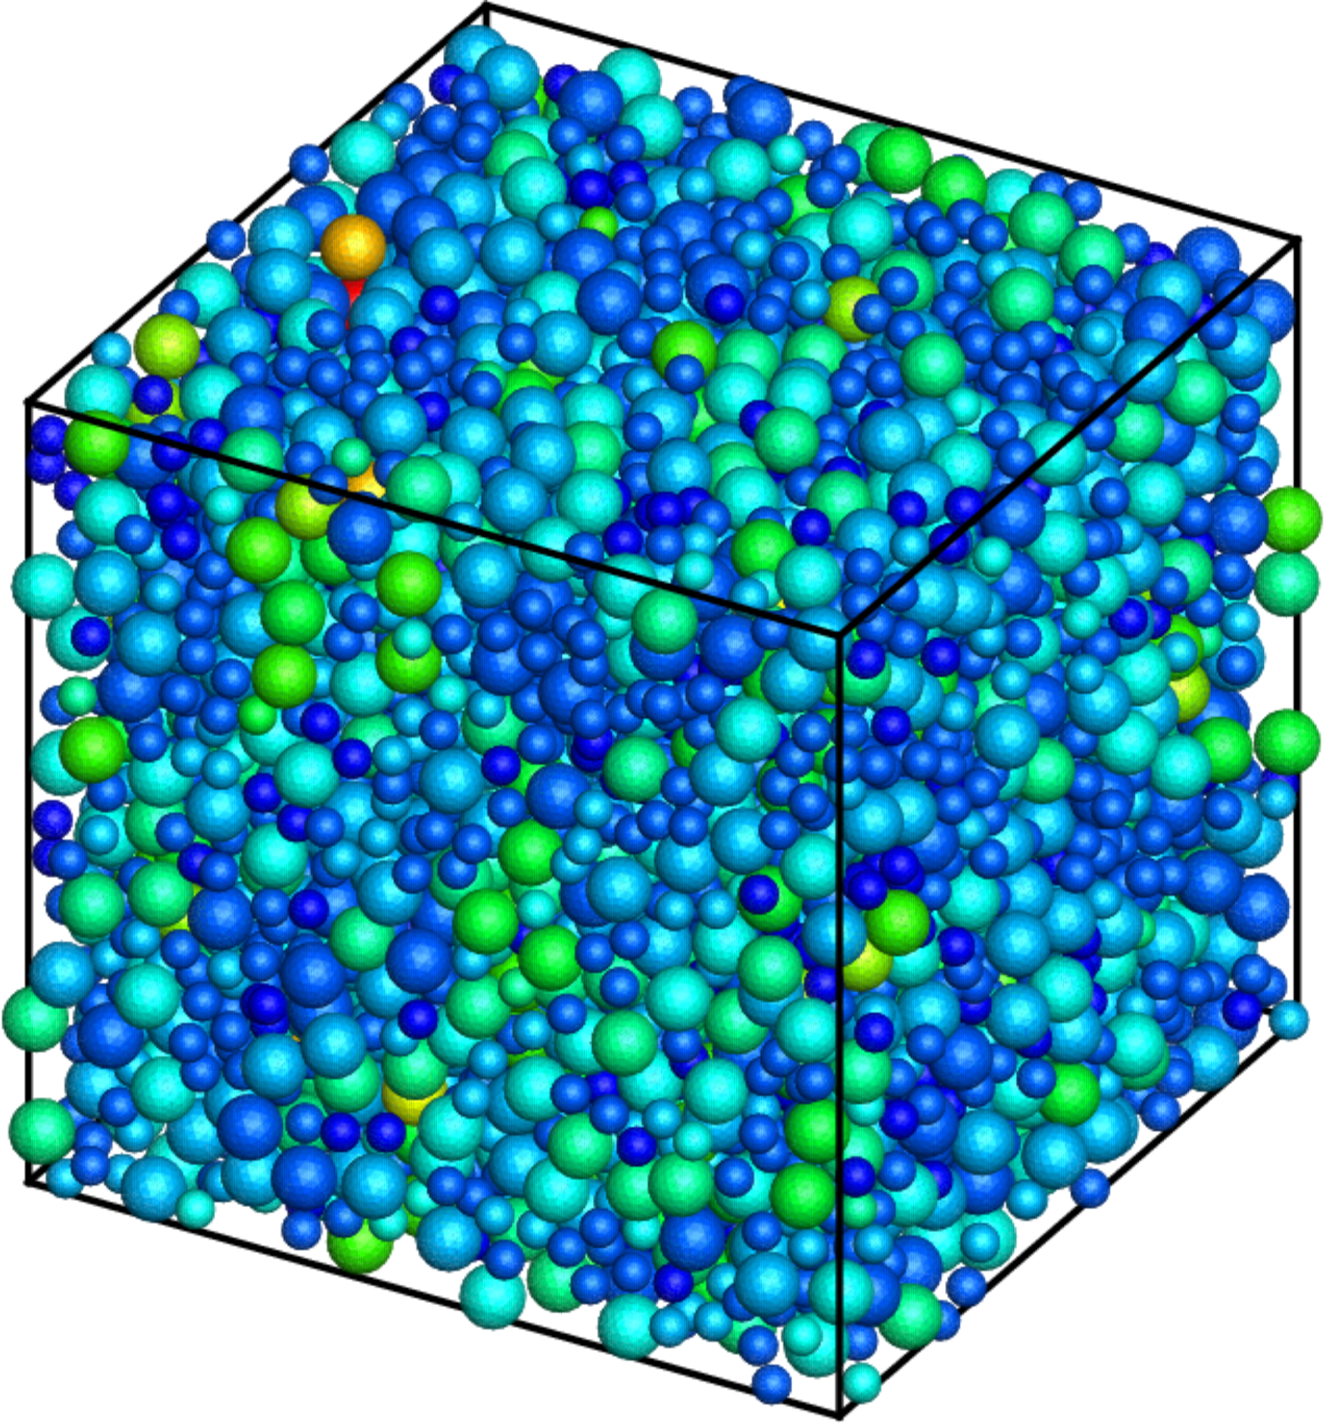
\includegraphics[width=6cm]{chapters/figures/Fig-3}
\begin{picture}(15,15)(340,-120)
\put(330,-80){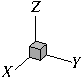
\includegraphics[scale=1]{chapters/figures/Fig-3b}}
\end{picture}
\end{minipage}
\end{center}
\caption{(color online) A binary pebble assembly with $\rstar = 0.6$ and $\vstar=0.7$ showing the stored elastic energy of the pebbles at $\epsilon_{33}=1.5\%$; pebbles of radius $r_s$ (small) and $r_g$ (large).}
\label{fig:pebble-assembly-potential-energy}
\end{figure}



\begin{figure}[!t]
  \begin{center}
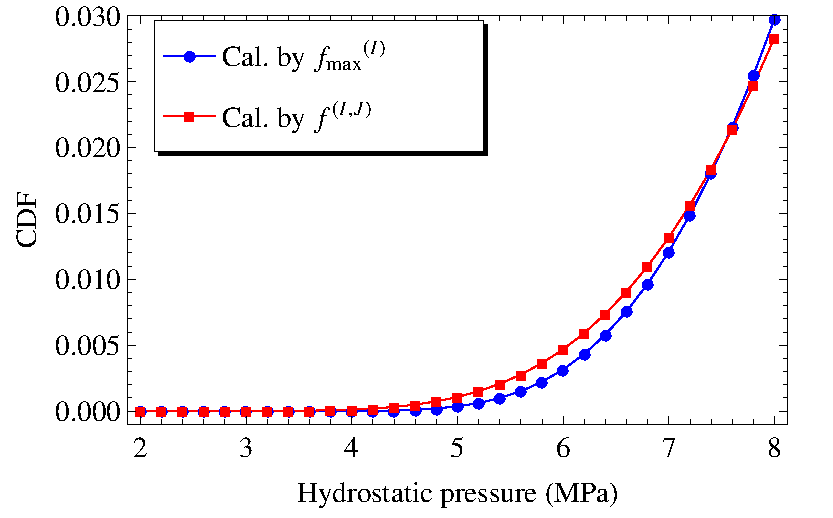
\includegraphics[width=0.5\textwidth]{chapters/figures/Fig-4}
\end{center}
 \caption{(color online) Cumulative distribution functions for crushing of individual pebbles inside the bed for as-fabricated pebbles, calculated by (1) maximum contact forces and (2) all inter-particle contact forces~\cite{Gan:2010kc}.}
 \label{fig:cdf_pebbles}
\end{figure}


\begin{figure}[t!]
\begin{center}
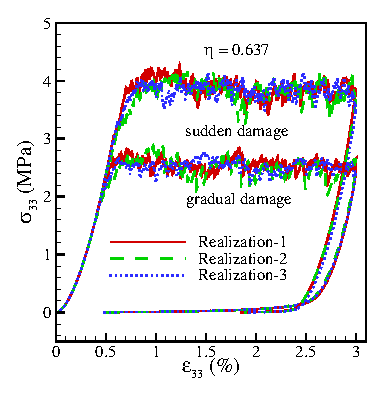
\includegraphics[width=0.4\textwidth]{chapters/figures/Fig-5}
\end{center}
\caption{(color online) Stress-Strain response of a granular assembly under uni-axial compression for two different damage evolution laws (gradual and sudden). Each damage evolution criterion is simulated with three different realizations of randomly prescribed critical failure energy for individual pebbles following Weibull distribution.}
\label{fig:stress-strain-effect}
\end{figure}



\section{Experimental Pebble Bed Thermomechanics Studies}
\subsection{Out-of-pile experiments}
The constitutive equations developed for finite element models were derived from the uniaxial compression experiments, which are not fully representative of fusion operating conditions. A more prototypical experiment should subject a pebble bed to isostatic loading. This could be generated by either an in-pile pebble bed experiment or by making use of differential thermal expansion between a pebble bed and its containing structure. The latter has been attempted with several out-of-pile experiments launched by the HE-FUS 3 facility at ENEA Brasimone. The experiments investigated the thermo-mechanical behavior of pebble beds within geometry much more representative of current breeder designs. These include the medium-scale mock-up exercises of HELICA (HE-FUS3 Lithium Cassette) and HEXCALIBER (HE-FUS3 Experimental Cassette of Lithium Beryllium Pebble Beds) \cite{dellorco:2006,DiMaio20081287}. For those experiments, the pebble layers are heated by electric heaters, and temperature and displacement were measured.

\subsubsection{FZK Benchmarking}
FZK has performed validation of their FEM code against the data collected from the HELICA experiment \cite{Gan:2008kx}. They have also reported the results of simulations of HEXCALIBER but have, as yet, not directly validated against the collected experimental data \cite{Gan:2009vn}.

In the HELICA experiment, the pebble beds experienced six thermal ramps, each applied for an hour, and then the pebble beds were actively cooled with a helium flow. After cooling, the pebble beds were subjected to the another thermal ramp and the process was repeated. DIN reports\cite{dellorco:2006} that the pebble bed temperatures exhibited cyclical behavior. FZK simulated two cycles of the HELICA test and an example of the calculated results and experimental data are shown in Fig.~\ref{fig:FZK_HELICAa} and Fig.~\ref{fig:FZK_HELICAb}. In Fig.~\ref{fig:FZK_HELICAa} we see temperature histories at a particular location (100 mm from the first wall) during a loading-unloading cycle. The simulation results follow the temperature increase during the thermal ramps up until the seventh hour, then again follow the experimental data as the test rig is cooled with the helium coolant. Even with the two-dimensional simplification of the model, there is excellent agreement between calculations and measurements. In Fig.~\ref{fig:FZK_HELICAb} the displacement calculated by FZK is also in strong agreement with the average of measured displacements for the entire duration of the heating-cooling cycle. Because of the overwhelming amount of computer time necessary for the FZK model to complete a fully three-dimensional and transient simulation, the FZK computations of HELICA and HEXCALIBER are carried out in two dimensions; the helium temperature is chosen at an average value of measured inlet and outlet temperatures.

From FZK's numeric simulation arise several important observations: (i) a three-dimensional analysis would provide more detail, spatial temperature variation of e.g. coolants would likely explain much of the deviation between temperature profiles predicted by the simulation and measured in the HELICA experiment; (ii) gap formations, with sizes on the order of a pebble diameter, were detected at the interface of the first wall in ceramic beds; (iii) the maximum hydrostatic pressures seen in the ceramic bed are anticipated to be above the fracturing limit of the lithium ceramic. The consequences of some of these observations, if true and real, are severe enough that they merit careful attention. Gap formation and pebble failure (crush or fracturing) are important topics that must be considered in validation with future experiments.

\subsubsection{DIN Benchmarking}
Because of the characteristics of the DIN model, full three-dimensional simulations were capable of being relatively easily performed. In the framework of benchmarking efforts, DIN has performed validation of their model against experimental results of HELICA, shown in Fig.~\ref{fig:DIN_HELICA} as well as HEXCALIBER, shown in Fig.~\ref{fig:DIN_HEX}.

The results of the DIN model show also strong agreement to the experimental results of HELICA as demonstrated in one example of temperature histories shown in Fig.~\ref{fig:DIN_HELICA}. In this profile, the same location as that modeled by FZK (100 mm from the first wall) is simulated by DIN. The FEM simulations from DIN (Fig.~\ref{fig:DIN_HELICA}) are reported over the six-hour heating portion of a single heating ramp cycle of HELICA. When comparing the results from DIN with those of FZK (in Fig.~\ref{fig:FZK_HELICAa} and Fig.~\ref{fig:FZK_HELICAb}) we see the DIN model has slightly better predictive capabilities for the temperature histories. This may be due attributed to the three-dimensional variations in coolant temperature being captured by the DIN model. 


\begin{figure}[t!]
\centering
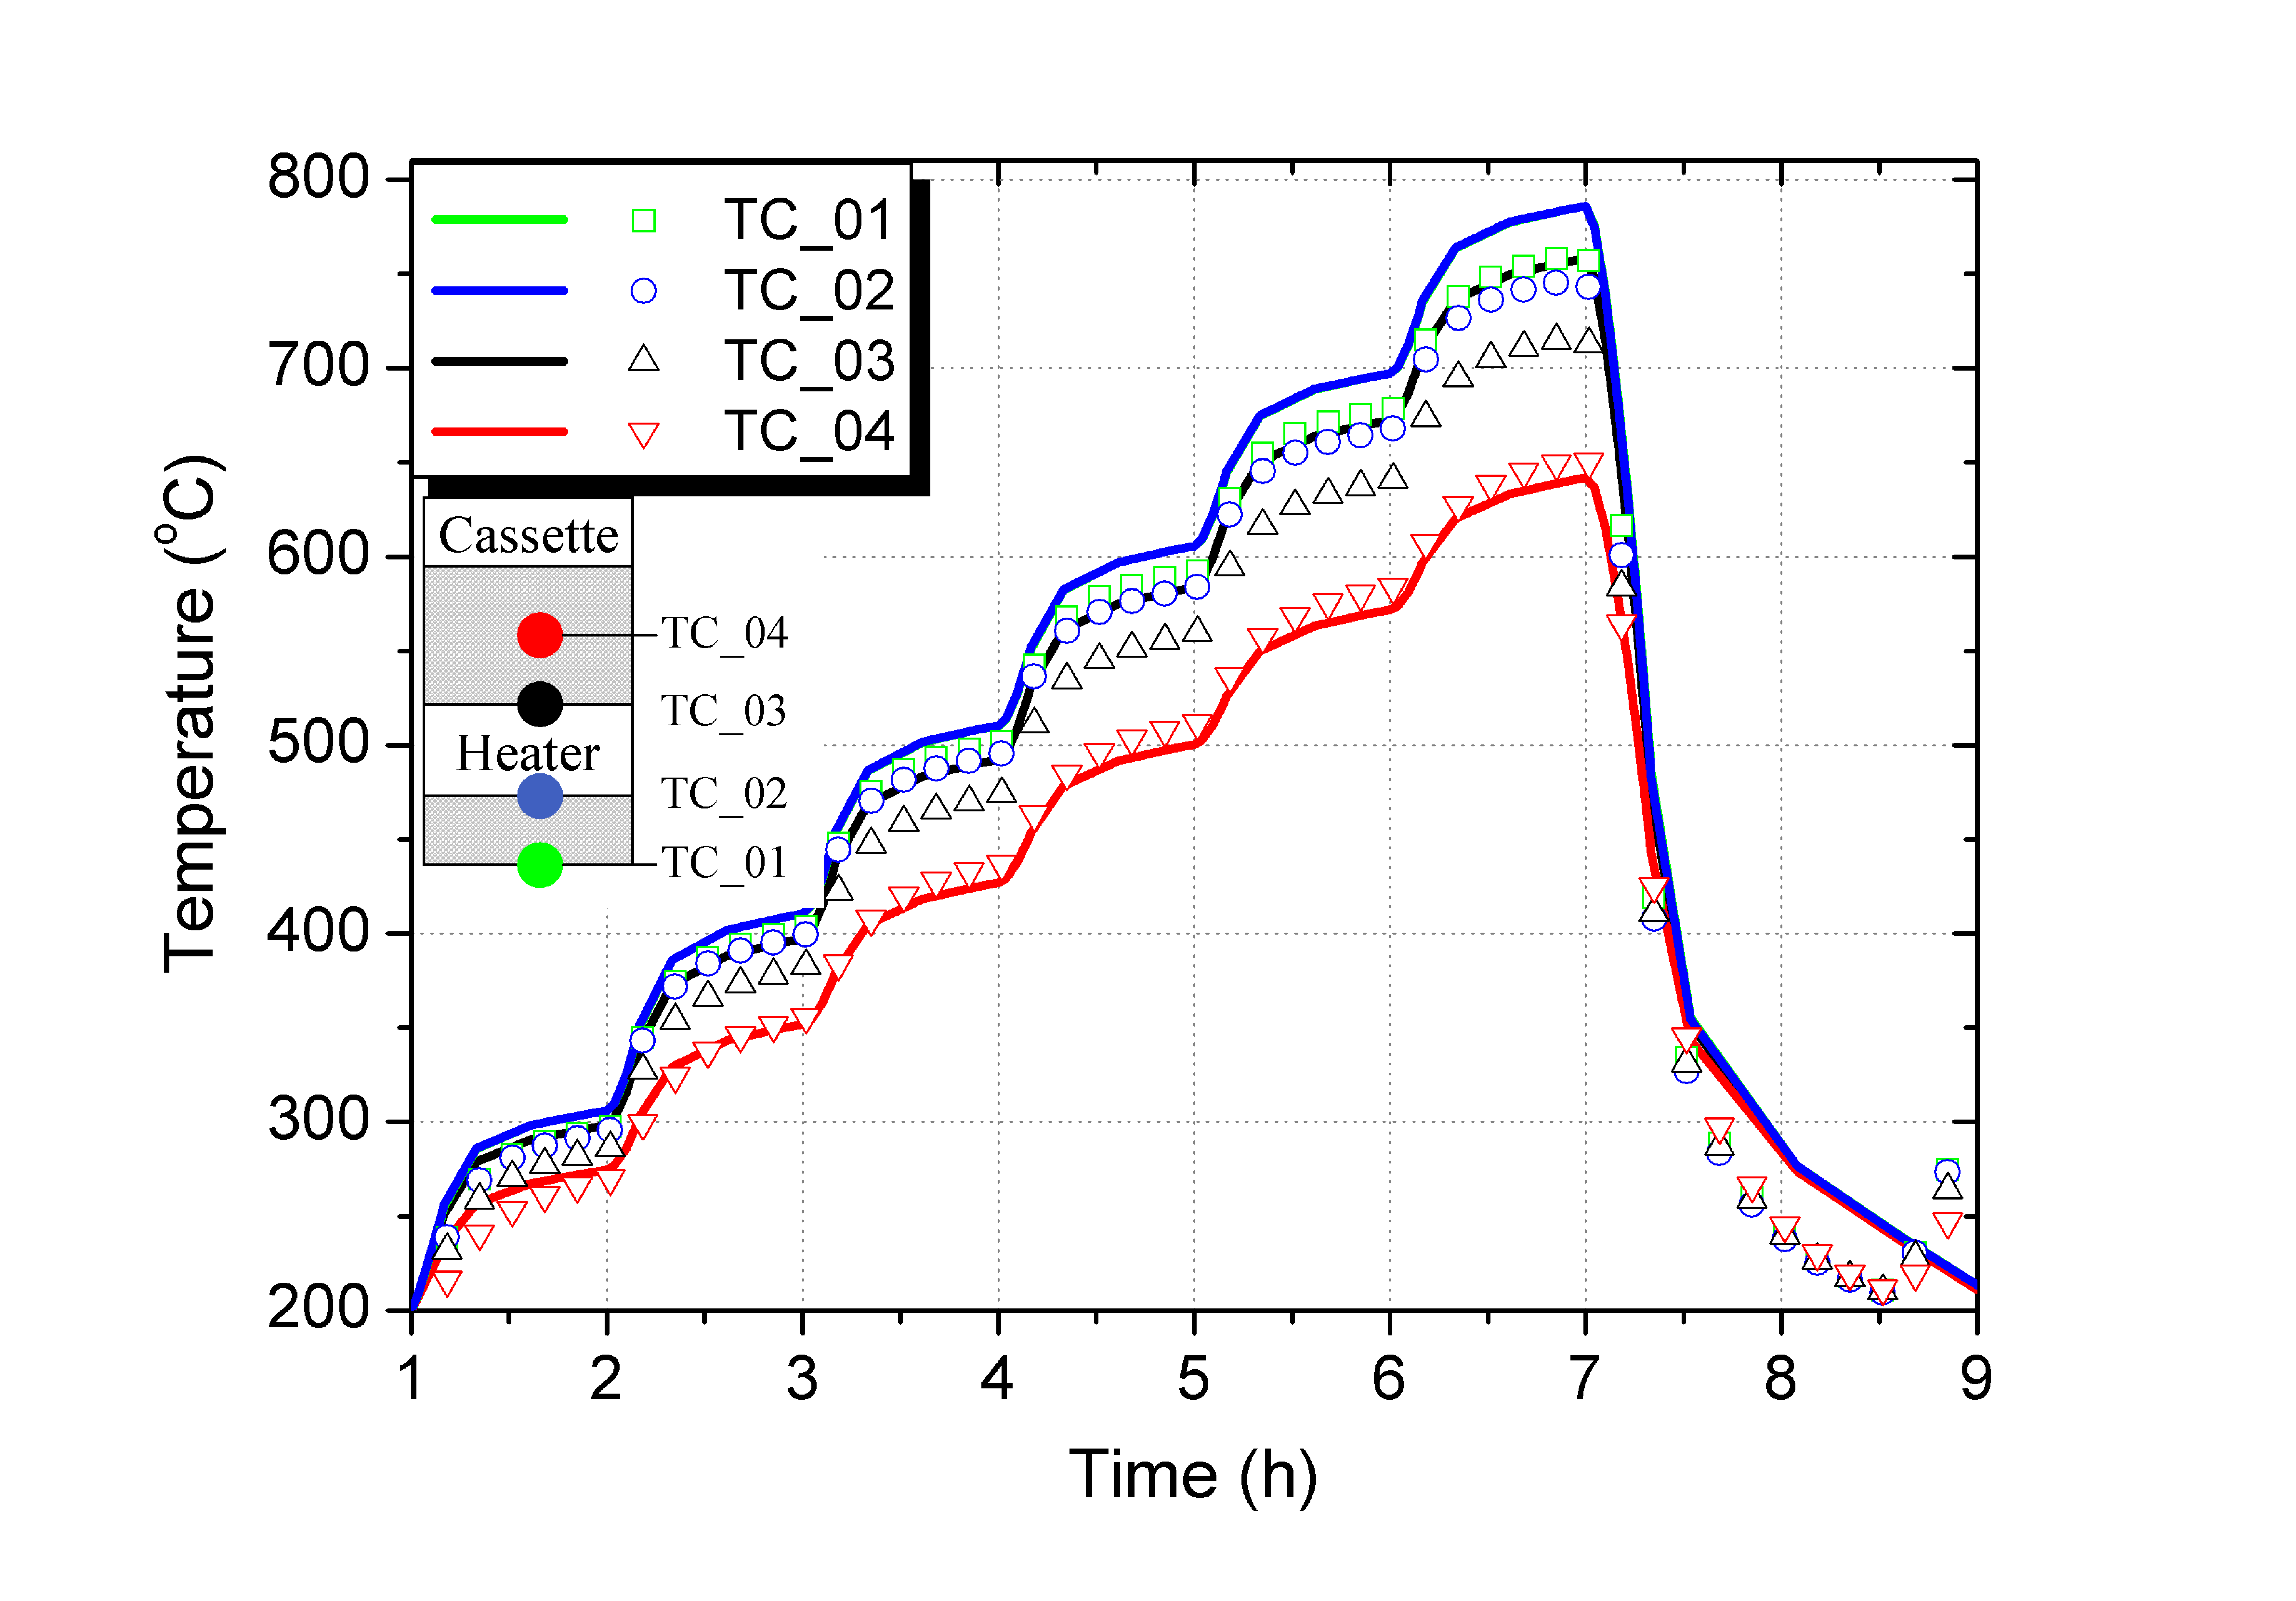
\includegraphics[width=0.5\textwidth]{chapters/figures/Fig-6}
\caption{Results of the FZK benchmarking with HELICA\cite{Gan:2009vn} showing temperature variations with time during a loading cycle (T in $^\circ$C) at 100 mm from FW.}\label{fig:FZK_HELICAa}
\end{figure}

\begin{figure}[t!]
\centering
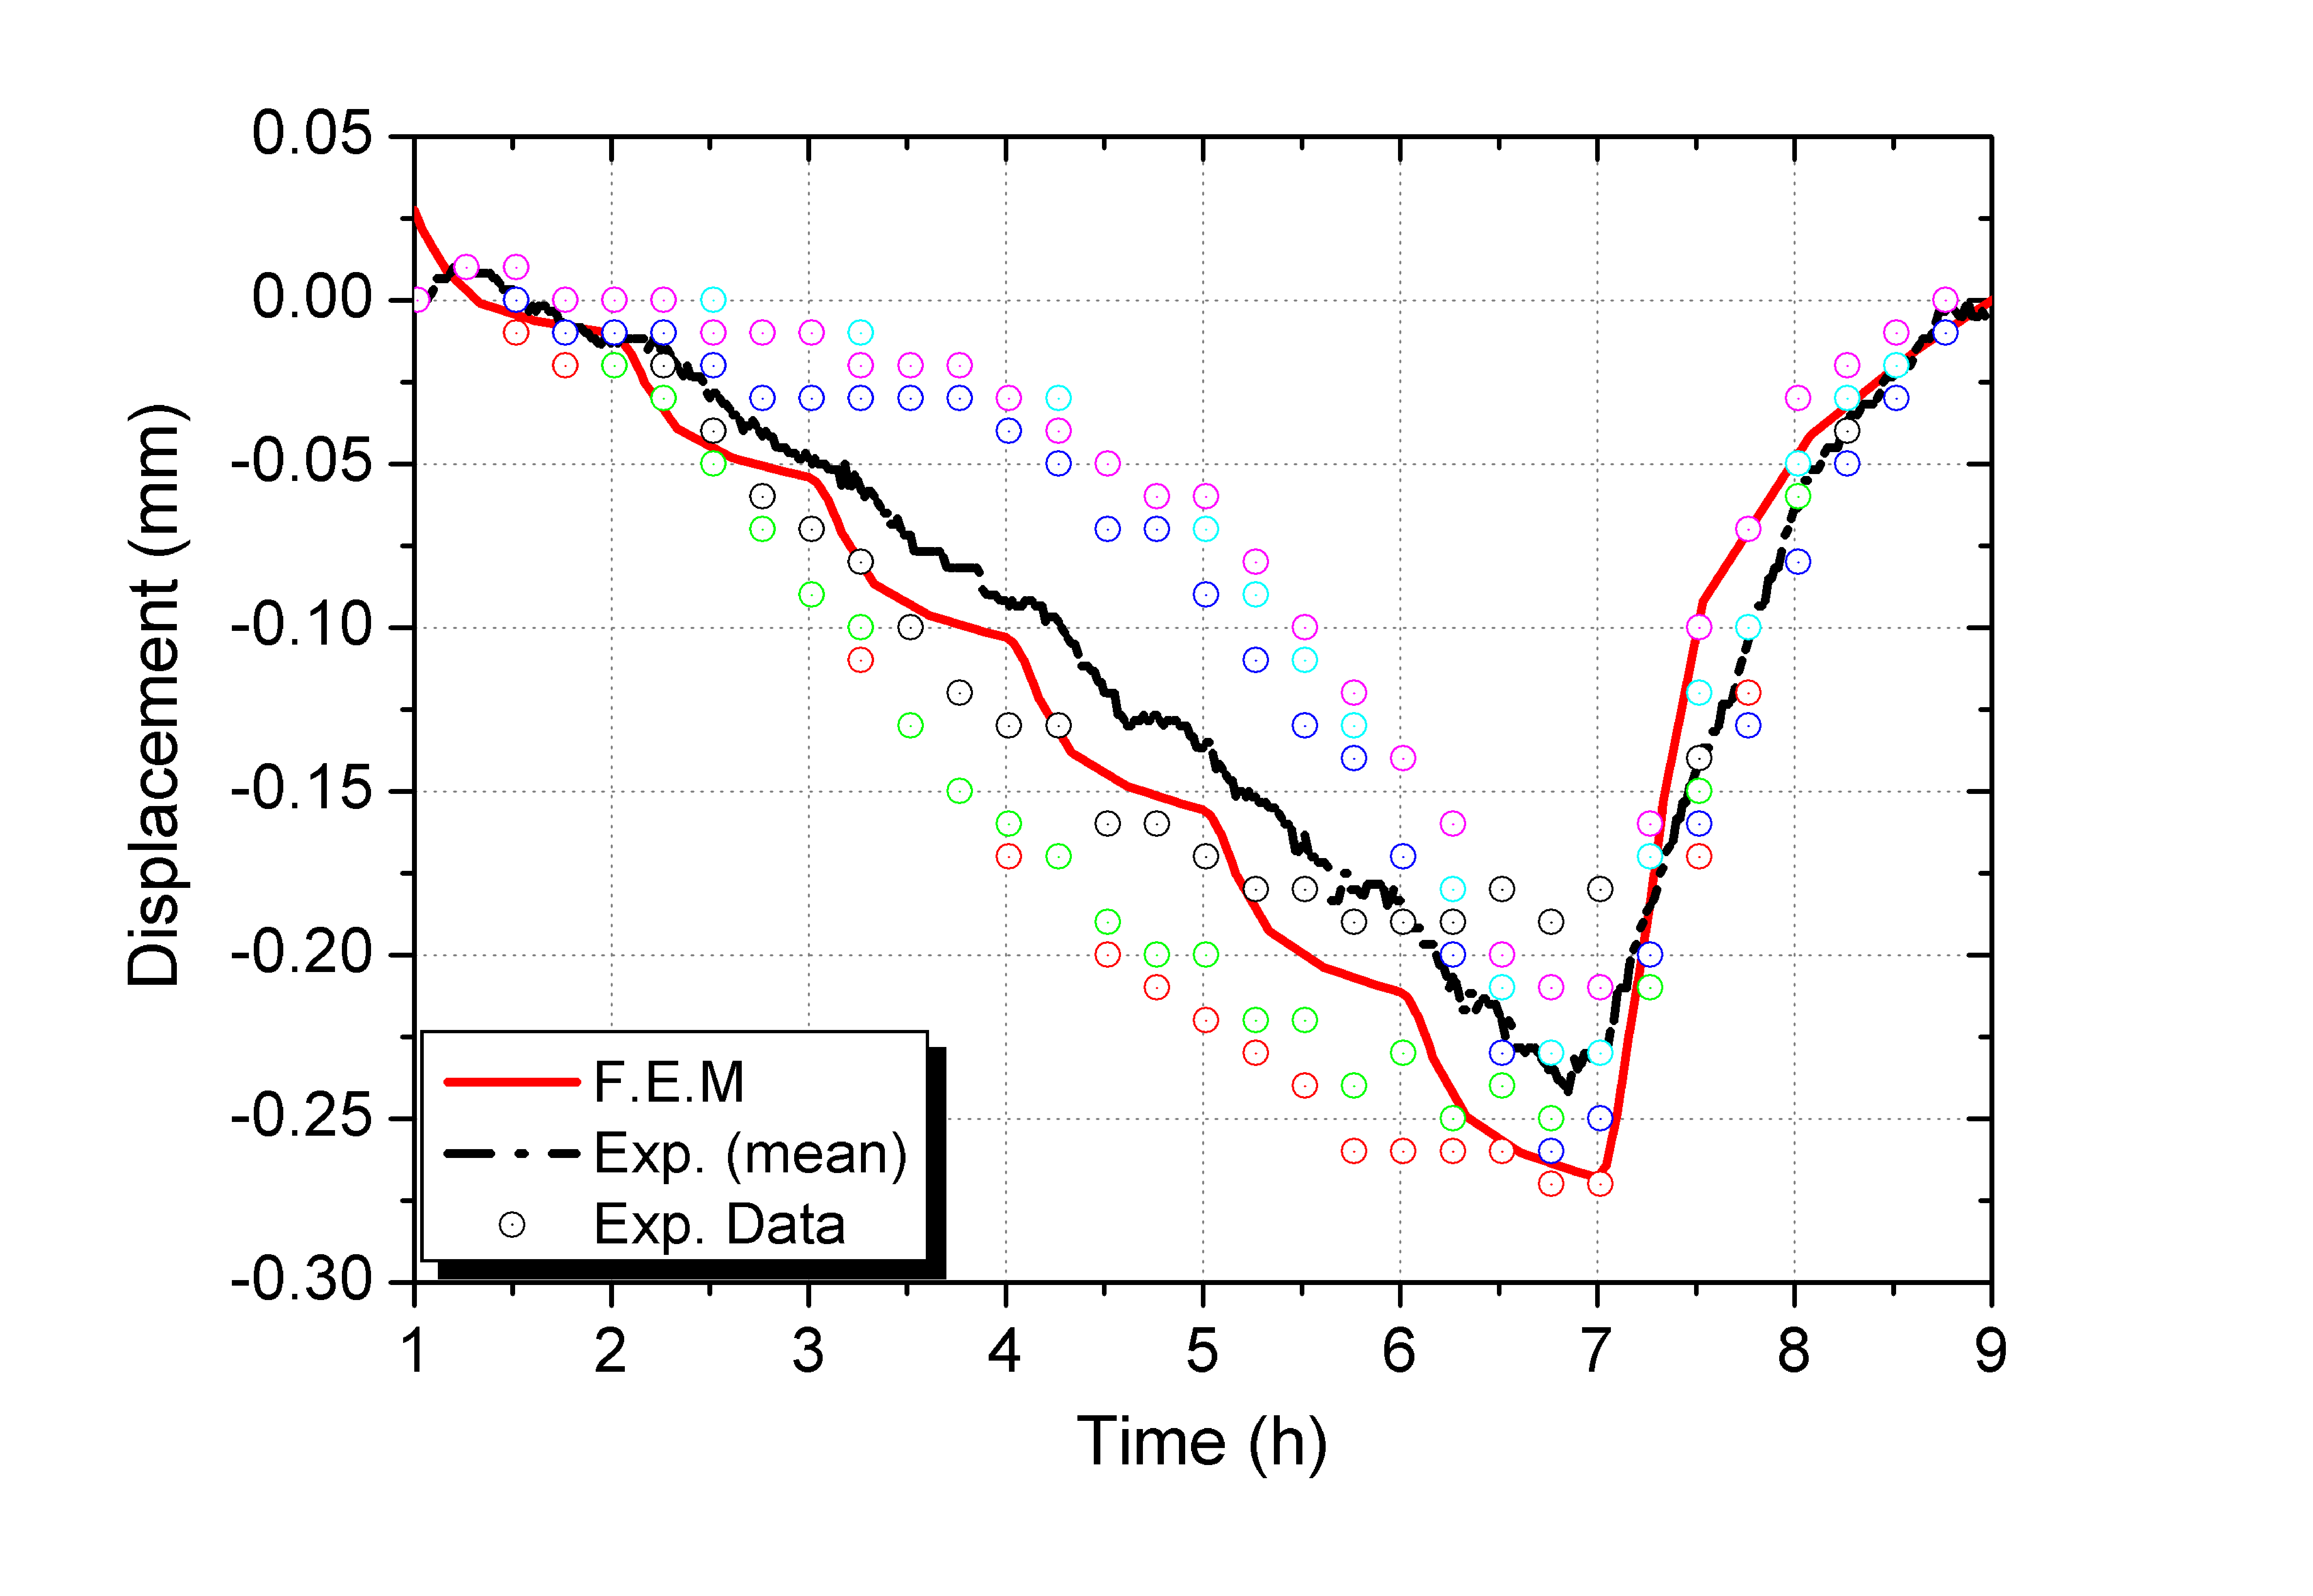
\includegraphics[width=0.5\textwidth]{chapters/figures/Fig-7}
\caption{Results of the FZK benchmarking with HELICA\cite{Gan:2009vn} showing a comparison of displacements (in mm) in HELICA between calculated and measured LVDT values.}
\label{fig:FZK_HELICAb}
\end{figure}

Unfortunately, the ambitions of HEXCALIBER were limited due to the crippling of several heaters. Nevertheless, the limited data was still used in efforts to validate the constitutive relationships of the DIN model. The temperature variations with time were the only major result reported by the ENEA Brasimone team, such as that shown in Fig.~\ref{fig:DIN_HEX}; mechanical results are still forthcoming from the research group. From the comparisons to experimental measurements in HELICA and HEXCALIBER it is encouraging to notice that even in the absence of a creep model, satisfactorily close agreement were seen between computation and measurement. So far, no detailed displacement comparisons have been made to experimental data.

Several important observations are also made from the results of the DIN simulation: (i) three-dimensional effects were important to calculations of the convective energy transport of the helium coolant; future models should continue to be analyzed in three-dimensions; (ii) DIN reports that in HELICA all ceramic beds experience a compressive force everywhere and no gap formation is ever detected. 

In summary, the benchmarking efforts have only recently begun in Europe. A typical pebble bed thermomechanics simulation involves first calculating overall temperature fields of the blanket unit as it undergoes volumetric nuclear heating as well as cooling at the boundaries. The non-linear mechanical analysis is then performed for stress and strain estimations. However, since the effective thermal conductivity of the ceramic breeder pebble bed is, to some degree, dependent on strain, a coupled thermal and mechanical analysis is needed. Additional details on modeling steps can be found in Refs.~\cite{DellOrco:2010zr,DiMaio20081287,DiMaio20101234,Gan:2009vn,Gan:2010lh,dellorco:2006}. The two most developed models, from FZK and DIN, have had their results compared to experimental data and have thus far shown great promise. 

However, it must be noted that the benchmarking efforts are incomplete and inconsistencies between the two models must be explained as they move forward. For example, the model of FZK concluded that a gap appeared between the pebble bed and structural wall, however the model from DIN reported no gap formation. The existence of a gap between pebble bed and structural wall will negatively affect the ability to cool the pebble bed and thereby impact structural and tritium release properties of the bed. That such a discrepancy exists between calculated results of the models on such a critical feature warrants either more benchmarking efforts or a careful deconstruction of the constitutive equations to discover the source of the inconsistency. Future experiments aimed at benchmarking ought to focus on creating apparatus capable of expressing, among other things, when gap formation or pebble failure occurs.


\begin{figure}[t!]
\begin{center}
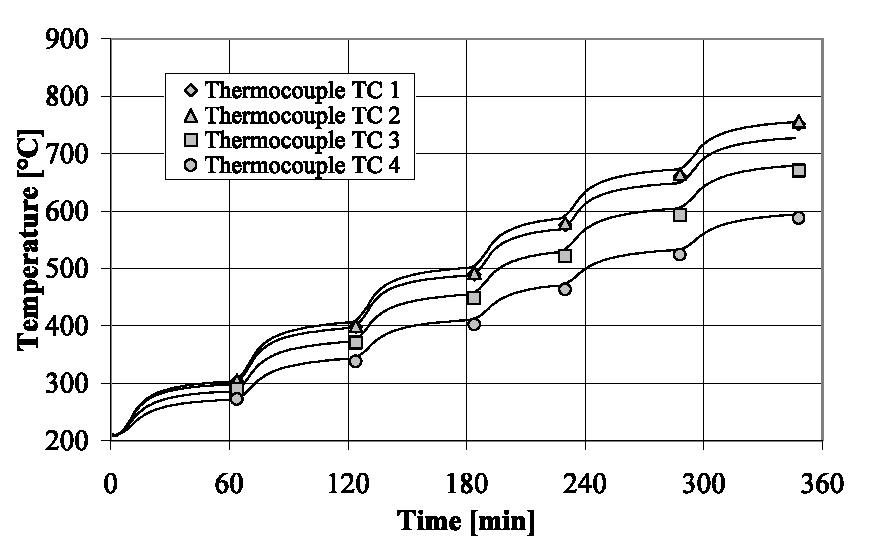
\includegraphics[width=0.4\textwidth]{chapters/figures/Fig-8}
\caption{Exemplary results of the DIN benchmarking with HELICA: Temperature variations with time during a loading cycle at 100 mm from FW\cite{DellOrco:2007hc}.}
\label{fig:DIN_HELICA}
\end{center}
\end{figure}


 \begin{figure}[t!]
\begin{center}
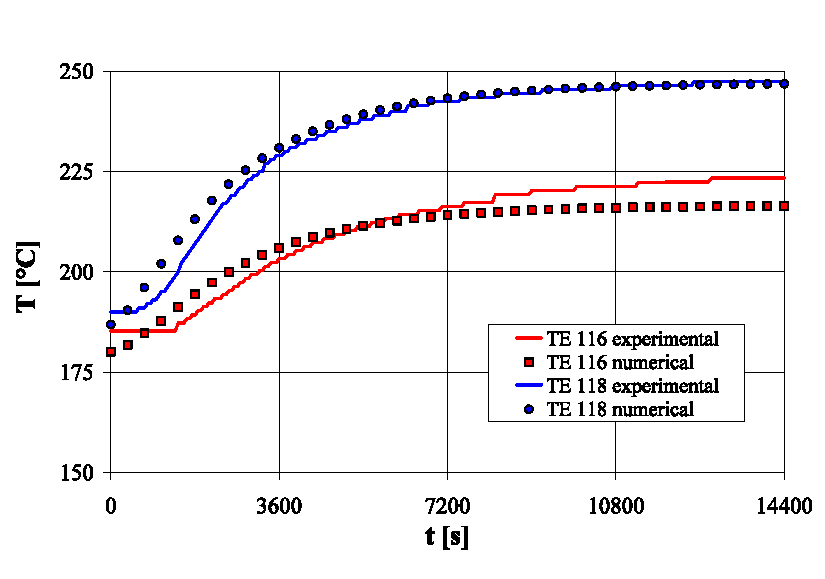
\includegraphics[width=0.4\textwidth]{chapters/figures/Fig-9}
\caption{Exemplary results of the DIN benchmarking with HEXCALIBER : Temperature variations with time during a loading cycle within the first lithium-orthosilicate cell\cite{DellOrco:2010zr}.}
\label{fig:DIN_HEX}
\end{center}
\end{figure}



\subsection{Pebble bed assemblies experiment}
The pebble bed assemblies (PBA) experiment is designed to study the effect of neutron irradiation on the thermo-mechanical behavior of a ceramic breeder pebble-bed under DEMO representative thermo-mechanical loads \cite{Magielsen2007,magielsen2005,sander2011}. This was accomplished via analysis of changes of the in-pile temperature profiles during irradiation as wall as from the post irradiation examination of the pebble bed in the Hot Cells. Within the assemblies, there are four test elements; each resembling a small-scale mock-up of a HCPB TBM with a ceramic breeder pebble bed sandwiched between two beryllium pebble beds. Before irradiation, the beds are pre-compacted with a compressive load of 3 MPa to ensure good settling and contact.  

FEM analysis was performed to study pre-compaction procedures.  During progressive irradiation, temperatures are recorded at several locations in the ceramic breeder bed as well as other critical positions. Reviewing the recorded temperature data, when comparing the temperature in the center of the ceramic breeder pebble bed during later cycles and earlier cycles there appears to be a decrease in temperature for the exact same environmental conditions. Changes in the pebble beds and their characteristics are examined both in-pile by neutron radiography and out-of-pile by e.g. SEM during post-irradiation examination (PIE). The estimated bed height reduction from neutron radiographies over the course of the irradiation has shown 3\% of creep compaction. 

A pebble bed experiencing creep compaction is both becoming more dense as well seeing more-developed inter-pebble conduction paths. The effective thermal conductivity for a creep-compacted ceramic pebble bed is thus expected to be higher than a standard ceramic pebble bed. This phenomenon results in lower temperature gradients and a lower overall temperature magnitude, which is precisely what was observed in the experiment over the course of the cycling. 

During PIE, various microscopy preparation techniques are used to study the deformation state of the pebble beds (signs of creep compaction and sintering), formation of gas gaps between the pebble beds and structural materials, and the interaction layers between eurofer-ceramic and eurofer-beryllium. 

Figure~\ref{fig:pba} shows the cross-section of Li$_2$TiO$_3$ pebbles (left) and Li$_4$SiO$_4$ pebbles (right) post irradiation. Evident in the images is sintering of the lithium titanite and significant fracturing of the lithium orthosilicate pebbles. Importantly, however, it must be noted that the pebble beds performed reliably in spite of the changes displayed in these images \cite{magielsen2011}. 


\begin{figure}[t!]
\centering
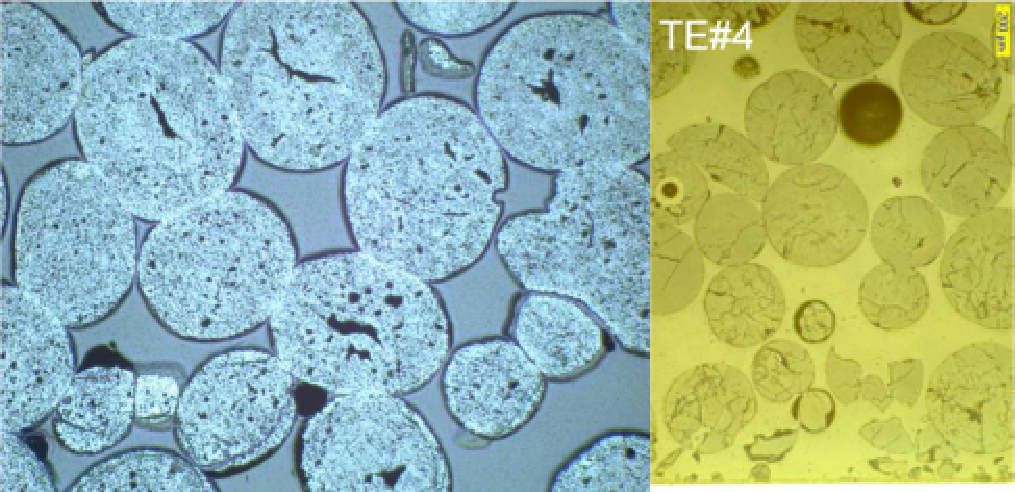
\includegraphics[width=0.5\textwidth]{chapters/figures/Fig-10}
\caption{Notable features of irradiated Li$_2$TiO$_3$ and Li$_4$SiO$_4$ pebble beds from PBA\cite{magielsen2011}. (Left) Demonstration of significant sintering of Li$_2$TiO$_3$ pebbles with no fracturing; the visible cracks originated from production and handling. (Right) Demonstration of cracking of Li$_4$SiO$_4$ pebbles.}
\label{fig:pba}
\end{figure}


\subsection{Other thermomechanics characterization experiments}
Coming from the standpoint that strain in a pebble bed is induced by thermal expansion, an experiment was conducted to characterize the pebble bed thermal expansion coefficient \cite{Tanigawa:2007fc}.  The thermal expansion coefficient of a packed \lit pebble bed is measured under a compressive load of 0.1MPa.  The study concludes that for beds with packing factors of 65.3 to 68.5\%, the average thermal expansion coefficient was $(1.4\pm0.2)\times10^{-5}K^{-1}$. This thermal expansion coefficient of the pebble bed was equal to 78\% of that for the bulk material under the conditions used in the study. The reduction in thermal expansion coefficient is less significant than that of the effective modulus, which is more than 2 orders of magnitude smaller than the bulk value. 

The effect of thermal cycling on the packing state is of interest; in particular, it is foreseen that the ITER TBM will be subjected to such conditions. The question that arises is whether a void region will be created under thermal-cyclic loading due to the differential rates of expansion and contraction of the pebble bed and structural containing wall. This uncertainty was first addressed in an experimental set-up involving Li$_2$TiO$_3$ pebbles enclosed by two Kovar flanges while sandwiched between two commercial-grade CVD silicon carbide discs \cite{Calderoni:2006ye}. The set-up allows for generating a high stress through large differential in thermal expansion coefficients. The experimental results indicate that high thermal stresses and deformations are present during the initial thermal cycle of the assembled test article, but are successively alleviated due to a combination of pebble re-arrangement within the bed and creep induced deformation. This suggests that a few thermal cycles under a controlled atmosphere and a compressive load before final assembly of blanket sections would mitigate the severity of the thermal stresses during start-up. This is also shown in a later experiment, in which the increment of compression decreased with each heating cycle and became negligible after 30 cycles \cite{Tanigawa:2010cr}. Extrapolating the finding to a prototypical blanket breeder pebble bed design, the study concludes that for a height of 1 m long pebble bed, a 51 mm high cavity may be generated at the top of the bed with an initial packing of 65\% under thermal cyclic operations.  

\section{Pebble Bed Thermomechanics Summary \& Framework}
The progress already achieved holds the promise of a pebble bed thermomechanics framework that will contribute substantially to the success of the ceramic breeder blanket development. In this framework, the continuum modeling approach using FEM and empirically derived material constitutive equations is capable of correctly characterizing the stress load to which a breeder pebble bed unit may be subject during the operations as shown in Fig.~\ref{fig:framework}. The DEM approach analyzes this load and determines the possibility fraction of pebble cracking based on the crush load data of pebbles or the degree of sintering depending on the local contact stress. The combined analyses warrants a high confidence of success to the assembly and design of breeder units in a blanket.  Experiments should also be conducted to assess the manner of pebble relocations and packing rearrangement when pebble cracking occurs. Since there is no perfect packing state, it is important to learn if the breeder unit will continue to function in accord with the original design goals under all complex operating conditions.  The ultimate objectives of the pebble bed thermomechanics include to delineate a  near-equilibrium packing state as the initial state, quantify breeder unit thermomechanics parameters during operations, understand how these properties vary as packing state alters and the degree of variation, and ensure breeder functions as it is intended to in the fusion operational phase spaces.
\begin{figure}[t!]
\begin{center}
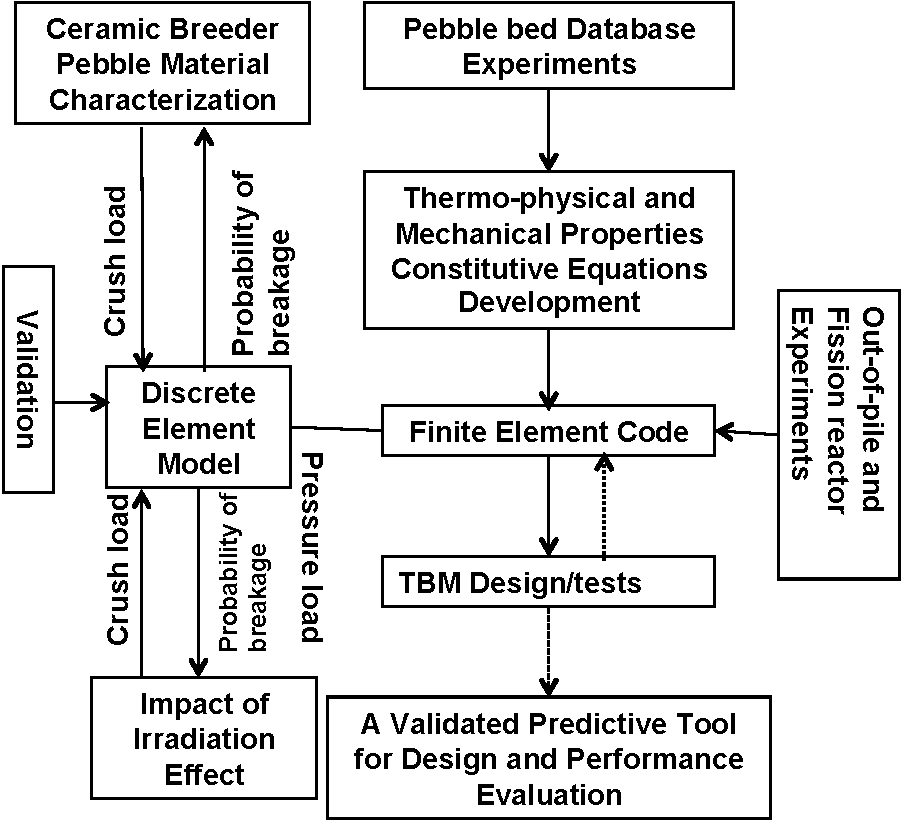
\includegraphics[width=0.5\textwidth]{chapters/figures/Fig-11}
\caption{Example Pebble Bed Thermo-mechanics Research Framework.}
\label{fig:framework}
\end{center}
\end{figure}

This leads to a more reliable blanket design. The analysis has preliminarily defined what peak stress values the breeder unit may be subjected to under the operations (e.g. $< 2-3$ MPa for Li$_4$SiO$_4$ or $< 5$ MPa for Li$_2$TiO$_3$). Since creep will lead to stress relaxation, further development incorporating creep models for high temperature DEM simulation is desired. This may increase the peak stress margin if stress relaxation is taken into account. Despite the scale of the experiments conducted so far, validation experiments are still necessary in regards to current continuum FEM models. Moreover, validation and refinement of simulations with regards to pebble damage crush properties are desired in particular in view of damage mechanisms.  There may be merits to perform crush load tests for irradiated pebbles at operating temperature ranges (room to 850/900 $^\circ$C). It holds forth promising on the continued pebble bed thermomechanics study in fine details a higher confidence to the ceramic breeder lifetime performance in a blanket.  The quest is to define and search a persistent ceramic breeder packing state throughout the blanket lifetime. 


% Methodology
% % Alice Comments:
% Does the contact force drop once the roughness is implemented?   How are we going to say about the large contact force, for example 5,9 N is a large number for Li4SiO4 pebble? Should I compare Eq. 3.29 with Eq. 3.16? The contact force disappears (or not apparent) in Eq. 3.29? Since there is a quite a significant drop in keff, discussions should be a bit details.  

% DONE Label for Fig. 3-16.  

%  You discuss E after thermal conductance section. What E do you use to get contact force of 5.9 N? 

% DONE I think the arrangement seems good. The title for Chapter 3 may need to change to include fragment study.  Like Construction of a Transient DEM for Solid-Solid Conductance and Packing Alteration Study (or without Construction of)? 

% DONE In Introduction you can then say this forms the basis for further development. Also, you don't use "spend some time" in a scientific paper. 




\chapter{Transient DEM Modeling of Solid-solid Contact Conductance and Packing Changes in Solid Breeder Pebble Beds}\label{ch:modeling-development}


In this chapter thorough descriptions of mechanical and thermal interactions internal to packed beds and their governing equations as implemented with the discrete element method are given. We start with establishing a kinematics framework which simply states that physical granular interactions obey Newton's laws of motion, and the motion of interactions is integrated in time. Contact mechanics models then dictate the normal and tangential forces of interacting grains that feed into the generic kinematic equations; the choice of contact model thus largely dictates the overall behavior of the granular material. Granular heat conductance models are implemented in DEM which, too, is reliant upon the contact force modeling. Application of DEM as a tool for measuring thermomechanical interactions between pebbles for solid breeders is validated \textit{via} numerical experiments to compare effective thermal conductivity with established measurements of effective thermal conductivity of lithium ceramic pebble beds. The contact model we use is based on Hertz's solution for elastic bodies, thus the elastic modulus of the grain is an important property for our models and we experimentally validate the application of Hertz Law; validation is possible with a new phenomenological model for the ceramic pebble elasticities. Lastly a technique for fragmentation modeling and investigate fragments and resettling in numeric ensembles is provided. The DEM model established in this chapter will form the basis for further development of tools for determining temperature distributions in solid breeder pebble beds.

%%%%%%%%%%%%%%%%%%%%%%%%%%%%%%%%%%%%%%%%%%%%%%%%%%%%%%%%%%%%%%%%%%%%%%%%%%%%%%%%%%%%%%%%%%%%%%%%%%%%%%%%%%%%
%%%%%%%%%%%%%%%%%%%%%%%%%%%%%%%%%%%%%%%%%%%%%%%%%%%%%%%%%%%%%%%%%%%%%%%%%%%%%%%%%%%%%%%%%%%%%%%%%%%%%%%%%%%%
%
% new section
%
%%%%%%%%%%%%%%%%%%%%%%%%%%%%%%%%%%%%%%%%%%%%%%%%%%%%%%%%%%%%%%%%%%%%%%%%%%%%%%%%%%%%%%%%%%%%%%%%%%%%%%%%%%%%
%%%%%%%%%%%%%%%%%%%%%%%%%%%%%%%%%%%%%%%%%%%%%%%%%%%%%%%%%%%%%%%%%%%%%%%%%%%%%%%%%%%%%%%%%%%%%%%%%%%%%%%%%%%%
\section{Grain-scale Modeling} \label{sec:modeling-dem}

The observable, macroscopic behavior of particulate, or granular, systems is a complex function of myriad particle interactions. Historically, empirical relationships have been used to describe these systems as if continuous media, \textit{e.g.} the correlations for heat transfer discussed in \Cref{sec:granular-ht-correlations}. But with the advent of the discrete element method by Cundall \& Strack and the acceleration of computing power, it became practical to investigate these granular materials at the particle scale without continuum assumptions \cite{Cundall1979}. With DEM, we track all the particles in the system in a Lagrangian manner. In the ensemble, the kinematics of each particle is tracked and updated based on balances (or imbalances) of forces or energy acting upon the particle. 


%~~~~~~~~~~~~~~~~~~~~~~~~~~~~~~~~~~~~~~~~~~~~~~~~~~~~~~~~~~~~~~~~~~~~~~~~~~~~~~~~~~~~~~~~~~~~~~~~~~~~~~~~~~~
% new subsection
%~~~~~~~~~~~~~~~~~~~~~~~~~~~~~~~~~~~~~~~~~~~~~~~~~~~~~~~~~~~~~~~~~~~~~~~~~~~~~~~~~~~~~~~~~~~~~~~~~~~~~~~~~~~
\subsection{Particle Dynamics}\label{sec:particle-dynamics}

The grains in our system are allowed translational and rotational degrees of freedom. In a packed bed, we can restrict our attention to local forces between particles; neglecting, say, non-contact forces such as, van der Waals, electrostatic, or for the time being any fluid interaction forces. Assuming we know the contact forces acting upon particle $i$, Newton's equations of motion are sufficient to describe the particle kinematics. For translation and rotational degrees of freedom, the equations are:,
\begin{subequations}
\label{eq:newtons-second}
\begin{align}
	m_i  \ddt{\vec{r}_i}   & = m_i\vec{g} + \vec{f}_i \label{eq:newton-translational} \\
	I_i\dt{\vec{\omega}_i} & = \vec{T}_i \label{eq:newton-rotational}
\end{align}
\end{subequations}
where $m_i$ is the particle mass, $\vec{r}_i$ its location in space, $\vec{g}$ is gravity, $I_i$ is the particle's moment of inertia, and $\vec{\omega}_i$ its angular velocity.

The net contact force, $\vec{f}_i$, represents the sum of the normal and tangential forces from the total number of contacts, $Z$, acting on this grain.
\begin{equation}
 	\vec{f}_i = \sum_{j=1}^{Z} \vec{f}_{n,ij} + \vec{f}_{t,ij}
 \end{equation} 
and the net torque, $\vec{T}_i$, is similarly,
\begin{equation}
	\vec{T}_i = -\frac{1}{2}\sum_{j=1}^{Z} \vec{r}_{ij} \times \vec{f}_{t,ij}
\end{equation}

When Cundall \& Strack first proposed the discrete element method, they used a linear spring-dashpot structure which saw normal and tangential forces written as,
\begin{subequations}
\label{eq:dem-forces}
\begin{align}
	\vec{f}_{n,ij} &= k_{n,ij} \delta_{n,ij}\vec{n}_{ij} - \gamma_{n,ij} \vec{u}_{n,ij} 	\label{eq:normal-force} \\
	\vec{f}_{t,ij} &= k_{t,ij} \delta_{t,ij}\vec{t}_{ij} - \gamma_{t,ij} \vec{u}_{t,ij} 	\label{eq:tangential-force}
\end{align}
\end{subequations}
where Cundall \& Strack defined the stiffness coefficients $k$ as constants and local damping coefficients $\gamma$ were proportional to them, $\gamma \propto k$, to allow dissipation of energy and the system to reach an equilibrium. 

Relative normal and tangential velocities, respectively, are decomposed from particle velocities,
\begin{subequations}
\label{eq:dem-velocities}
\begin{align}
	\vec{u}_{n,ij} &= (-(\vec{u}_i-\vec{u}_j)\cdot\vec{n}_{ij})\vec{n}_{ij} \\
	\vec{u}_{t,ij} &= (-(\vec{u}_i-\vec{u}_j)\cdot\vec{t}_{ij})\vec{t}_{ij}
\end{align}
\end{subequations}
with the unit vector $\vec{n}_{ij}$ pointing from particle $j$ to $i$

As in the solution of Hertzian interaction (see \Cref{sec:hertz-theory}), the surfaces of the two particles are allowed to virtually pass through each other (no deformation) resulting in normal and tangential overlaps of,
\begin{subequations}
\label{eq:dem-overlaps}
\begin{align}
	\delta_{n,ij} &= (R_i + R_j) - (\vec{r}_i -\vec{r}_j)\cdot \vec{n}_{ij} \\
	\delta_{t,ij} &= \int_{t_{c,0}}^{t} \vec{u}_{t,ij}\,\mathrm{d}\tau 
\end{align}
\end{subequations}
where the fictive tangential overlap, $\delta_{t,ij}$, is truncated to so the tangential and normal forces obey Coulomb's Law, $\vec{f}_{t,ij} \le \mu_i \vec{f}_{n,ij}$ with $\mu$ as the coefficient of friction of the particle.

Thus the approach of DEM is relatively simple: calculate interaction forces between particles with \Cref{eq:dem-forces} based on the kinematics of velocity and position of interacting particles from \Cref{eq:dem-velocities} and \Cref{eq:dem-overlaps}, respectively, then update the positions based on the forces. As DEM evolved and drew attention of more researchers, more complex formulas governing the spring-dashpot coefficients of \Cref{eq:dem-forces} emerged. But the core approach remained the same and the models all fall into the same family of so-called `soft particle' models of DEM. A well-composed summary of the different DEM force models is given by Zhu\etal.\cite{Zhu2007}

The method used in this work fits into the computational skeleton of Cundall and Strack's method but with non-linear spring-dashpot coefficients defined by simplified Hertz-Mindlin-Deresiewicz model. In this model, the normal-direction stiffness coefficient of \Cref{eq:normal-force} is based on the Hertzian contact law (derived explicitly in \Cref{sec:hertz-theory}). The validity of Hertzian descriptions of normal forces is tested experimentally and reported in \Cref{sec:exp-reduction-factor}.The tangential-direction stiffness coefficient follows from Brilliantov \cite{Brilliantov1996, Zhu2007, Langston1995}. Together, the spring coefficients are,
\begin{subequations}
\begin{align}
	k_{n,ij} &= \frac{4}{3}E_{ij}^*\sqrt{R_{ij}^*\delta_{n,ij}} \\
	k_{t,ij} &= 8 G_{ij}^*\sqrt{R_{ij}^*\delta_{t,ij}}
\end{align}
\end{subequations}
where $E_{ij}^*$ is the pair elastic modulus, $G_{ij}^*$ is the pair bulk modulus, and $R_{ij}^*$ is the relative radius. The terms are defined as,
\begin{subequations}
\begin{align}
	\frac{1}{E^*} &= \frac{1-\nu_1^2}{E_1} + \frac{1-\nu_2^2}{E_2} \\
	\frac{1}{R^*} &= \frac{1}{R_1} + \frac{1}{R_2} \\
	\frac{1}{G^*_{ij}} &= \frac{2(2+\nu_i)}{E_i} + \frac{2(2+\nu_j)}{E_j}
\end{align}
\end{subequations}

Similar to Cundall \& Strack's formulation, damping coefficients, $\gamma$, are included to account for energy dissipated from the collision of two particles \cite{DiRenzo2004, Tsuji1992, Tsuji1993}. Whether the damping coefficient is local or global and the exact form of the coefficient is more important for loosely confined granular systems and dictates the way the system approaches an equilibrium state \cite{Makse2004}. For the case of our tightly packed pebble beds, it suffices to use the efficient form of Refs.\cite{Dippel1996, Makse2004, Brilliantov1996, Zhang2005, Zhu2007},
\begin{subequations}
\begin{align}
	\gamma_n &= \sqrt{5}\beta_\text{diss}\sqrt{m^*k_{n,ij}} \\
	\gamma_t &= \sqrt{\frac{10}{3}}\beta_\text{damp}\sqrt{k_{t,ij} m^*}
\end{align}
\end{subequations}
with $\beta_\text{damp}$ as the damping ratio, and the pair mass, $\frac{1}{m^*} = \frac{1}{m_i} + \frac{1}{m_j}$. For a stable system with $\beta_\text{damp} < 1$, the damping ratio is related to the coefficient of restitution, $e$, as
\begin{equation}
	\beta_\text{diss} = -\frac{\ln{e}}{\sqrt{\ln^2{e}+\pi^2}}
\end{equation}

Systems to be solved by DEM models are therefore well-defined after specifying the few material properties of $E$, $\nu$, $\rho$, and $R_p$ and the interaction properties of $\mu$ and $e$.

Having expressed the contact mechanics of the discrete element method, we now must integrate the kinematic equations of the particles to resolve their evolutions. The most common means of marching in time with DEM is the velocity-Verlet algorithm \cite{Kruggel-Emden2008}. In this algorithm, \Cref{eq:newtons-second} are integrated with half-steps in velocity, full steps in position, and then finally the full step in velocity. In practice, the two half-steps in velocity are often compressed into a single, full step. The computational time integration steps are given in explicit detail in \Cref{sec:dem-stability}. Owing to the explicit nature of the velocity-Verlet algorithm, stability is a constant concern with DEM simulations. Stable, critical time steps and practical means of circumventing unreasonably small time steps are discussed in \Cref{sec:dem-stability}.

A last note. Throughout this work, we required a fully quiesced bed to act as a starting point or demarcate a mechanically steady-state bed. To determine when this occurs, the total kinetic energy of the entire ensemble is monitored and a packed bed is considered to have completely settled once the magnitude of the system's kinetic energy is less than $10^{-8}$. A similar process was independently determined in a similar matter in the work of Ref.~\cite{Silbert2002}. 



%~~~~~~~~~~~~~~~~~~~~~~~~~~~~~~~~~~~~~~~~~~~~~~~~~~~~~~~~~~~~~~~~~~~~~~~~~~~~~~~~~~~~~~~~~~~~~~~~~~~~~~~~~~~
% new subsection
%~~~~~~~~~~~~~~~~~~~~~~~~~~~~~~~~~~~~~~~~~~~~~~~~~~~~~~~~~~~~~~~~~~~~~~~~~~~~~~~~~~~~~~~~~~~~~~~~~~~~~~~~~~~
\subsection{Granular Heat Transfer in DEM}\label{sec:dem-heat-transfer}

In a way analogous to handling particle momentums with Newton's laws of motion, Lagrangian tracking of particle energy is obtained \textit{via} the first law of thermodynamics. Each particle is treated as a single distinct object and thus internal temperature gradients are assumed negligible. The temperature of particle $i$ is governed by
\begin{equation}\label{eq:thermoFirstLaw}
	m_iC_i\dt{T_i} = Q_{s,i} + Q_{i}
\end{equation}
where $m$ and $C$ are the mass and the specific heat of the solid, respectively. Heat generation inside the particle is input with $Q_{s}$ and the total heat transferred to/from particle $i$ \textit{via} conduction to all, $Z$, neighboring particles, is
\begin{equation}
	Q_i = \sum_{j=1}^Z Q_{ij}
\end{equation}

Assuming the particles are spherical, smooth, elastic, in vacuum, and we neglect radiation transfer between them, for two particles at temperatures $T_i$ and $T_j$, we quantify the amount of energy transferred between them with a contact conductance, $H_c$:
\begin{equation}\label{eq:pebble-conduction-heat-transfer}
    Q_{ij} = H_{c}(T_i - T_j)
\end{equation}

Batchelor \& O'Brien\cite{Batchelor1977} developed a formulation of similar form and then made a brilliant observation that ``\textit{when the radius of the circle of contact is so large that the heat flux through the thin annular matrix layer is negligible by comparison with that through the contact circle, the distribution of temperature inside the two particles is approximately the same as that of the velocity potential in irrotational flow of incompressible fluid through a circular hole in a plane wall.}'' With the analogy, they made use of the fluid flow solution to write the total heat flux across the circle of contact as \Cref{eq:pebble-conduction-heat-transfer} with heat conductance 
\begin{equation}\label{eq:batchelor-pebble-conductance}
    H_c = 2k_sa
\end{equation}
where $k_s$ is the conductivity of the contacting solids and $a$ is the radius of contact. Because we have assumed smooth, elastic, spherical solids, with Hertz theory (see \Cref{sec:hertz-theory}), contact radius can be found as a function of contact normal force, $F_n$,
\begin{equation}
    a =  \left(\frac{3}{4}\frac{R^*}{E^*}\right)^{1/3}F_n^{1/3} 
\end{equation}
where, as before, $\frac{1}{E^*} = \frac{1-\nu_1^2}{E_1} + \frac{1-\nu_2^2}{E_2}$ and $\frac{1}{R^*} = \frac{1}{R_1} + \frac{1}{R_2}$. 

In the development of \Cref{eq:batchelor-pebble-conductance}, Batchelor \& O'Brien had assumed the two contacting spheres to be of equal conductivity, $k_s$. Cheng\etal\cite{Cheng19994199} proposed a slightly modified conductance which allows for contacting materials of different thermal conductivity. They give,
\begin{equation}\label{eq:cheng-modification-batchelor}
    H_c = 2k^*a = 2k^* \left(\frac{3}{4}\frac{R^*}{E^*}\right)^{1/3}F_n^{1/3}
\end{equation}
where $\frac{2}{k^*} = \frac{1}{k_i} + \frac{1}{k_j}$. As well as being a more general, flexible formulation, the models analyzed by Cheng\etal\cite{Cheng19994199} are in good agreement with experiments.

The condition for validity of Batchelor \& O'Brien's formulation of \Cref{eq:batchelor-pebble-conductance} is in the limit where $\Psi \rightarrow \infty$, where \cite{Batchelor1977}
\begin{equation}\label{eq:conductance-validity-fluid}
    \Psi = \frac{a}{R^*} \kappa
\end{equation}
The term $\frac{a}{R^*}$, from \Cref{sec:hertz-theory}, is necessarily less than 1 for Hertz theory to be applicable. Thus for fluid in vacuum, the condition is identically satisfied but we must consider inaccuracies if we introduce an interstitial fluid with low conductivity ratios; for lithium ceramics in helium, the ratio is approximately $\kappa \approx 10$.

We step back from contact of a single pair of particles and consider a particle in an ensemble with many contacts. We must again consider the validity of applying \Cref{eq:cheng-modification-batchelor} at each contact. Vargas and McCarthy\cite{Vargas2002a}, propose introducing a conduction Biot number to relate resistance of heat transfer internal to a particle with resistance between particles,
\begin{equation}
    \Bi_c = \frac{H_c}{k^* d_p} = 2\frac{a}{d_p}
\end{equation}

Then if $\Bi_c \ll 1$, the individual energy transferred between each point of contact can be decoupled. The Biot number criteria is already satisfied for Hertz theory to be valid; having assumed that $\frac{a}{d_p} \ll 1$. Therefore the total heat transferred out of a single particle with $Z$ contacts, due to contact conductance, is the summed contribution of individual contacts, 
\begin{equation}
    Q_i = \sum_j^Z Q_{ij}
\end{equation}

For the case when we do \textit{not} have a perfectly smooth elastic sphere, we use the approach of Bahrami\etal, introducing a joint thermal resistance to develop a modified heat conductance term. Bahrami\etal\cite{Bahrami2004} use a joint thermal resistance of the superposition of macroscopic and microscopic influences; the thermal joint resistance is
\begin{equation}
	R_j = R_s + R_L
\end{equation}
where the subscript $L$ refers to macroscopic variables and $s$ refers to microscopic ones. Bahrami\etal~used the constriction formulation of Yovanovich\etal~to express the macroscopic resistance as\cite{Yovanovich1976}
\begin{equation}
	R_L = \frac{(1-a/R^*)^{3/2}}{2k_sa}
\end{equation}
If the contact of the two materials obeys Hertz contact law, then $a/R^* \ll 1$ and the above becomes
\begin{equation}\label{eq:macro-thermal-resistance}
	R_L = \frac{1}{2k_sa}
\end{equation}
which matches the heat conduction form of Batchelor \& O'Brien\cite{Batchelor1977}, \Cref{eq:batchelor-pebble-conductance}.

To determine the thermal resistance of the asperities in contact, Bahrami\etal~used a superposition of many cylindrical constrictions inside of the contact area. The result is given in \cite{Bahrami2004} as
\begin{equation}
	\psi_s^* = \begin{cases}
	\left(\frac{\pi H'R^{*2}}{F} \right)^s 										& F_c = 0\\
	(R^*/a)^2(H'/P_0)^s(1+s\gamma) 										& F \le F_c\\
	(H'/P_{0,c})^s(1+s\gamma_c)+\left[\frac{\pi H'R^{*2}}{(F-F_c)}\right]^s				& F\ge F_c
	\end{cases}
\end{equation}
where $\psi_s^*$ is a non-dimensional form of the surface roughness thermal resistance, defined as $\psi_s^* = 1.25\pi R^{*2}k^*(m/\sigma)\psi_s$, $k^*$ is the harmonic mean of contact grains thermal conductivity, $H'$ is the Vicker's microhardness value, $F$ is the contact force, $P_0$ is the maximum pressure of contact, $s$ is a parameter based on the hardness constants, $\gamma = 1.5(P_0/P_{0,H})(a/a_H)^2-1$, $F_c$ is the critical force where $a = R^*$, $\gamma_c$ is the value of $\gamma$ at the critical force, $m$ is the mean absolute surface slope, and $\sigma$ is the root-mean-square (rms) surface roughness. For Hertzian contact, $\gamma = 0.5$.

Antonetti\etal~ proposed a correlation for mean absolute surface slope related to surface asperities as\cite{Antonetti1984}
\begin{equation}\label{eq:m-of-sigma}
	m = 0.125(\sigma\times10^6)^{0.402}
\end{equation}
where the range of applicability of surface roughness is \SI{0.216E-6}{\meter}$\le \sigma <$ \SI{9.6E-6}{\meter}. Thus the term $\sigma/m = 0.031\sigma^{0.598}$

For Hertzian contacts of the non-conforming ceramic materials, $F \ll F_c$, thus we consider only that case to write
\begin{equation}
	R_s = \frac{(R^*/a)^2(H'/P_0)^s(1+s/2)}{1.25\pi R^{*2}k^*(0.031\sigma^{0.598})}
\end{equation}
or
\begin{equation}\label{eq:thermal-resistance-pressure}
	R_s = \frac{(H'/P_0)^s(1+s/2)}{1.25\pi a^2k^*\left(0.031\sigma^{0.598}\right)}
\end{equation}
For Hertzian contact, the maximum pressure is given by \Cref{eq:hertzian-pressure}. It is
\begin{equation*}
	P_0 = \frac{2E^*\delta_n}{\pi a}
\end{equation*}
Furthermore, as noted by Bahrami\etal, the parameter $s$ is in the range of $0.95\le s\le 0.97$. Therefore it is approximated as $s=0.96$ here. The thermal resistance of \Cref{eq:thermal-resistance-pressure} is rewritten in a simplified form,
% \begin{equation}
% 	R_s = \frac{\pi^{s-1}}{1.25(2^s)}\left(\frac{H'}{E^*}\right)^s\frac{1+s/2}{k^*\delta_n^s}\left(\frac{\sigma}{m}\right)a^{s-2}
% \end{equation}
\begin{equation}\label{eq:micro-thermal-resistance}
	R_s = \left(\frac{H'}{E^*\delta_n}\right)^{0.96}\left(\frac{\sigma}{m}\right)\frac{1}{1.720k^*a^{1.04}}
\end{equation}

The macroscopic and microscopic thermal resistances given in \Cref{eq:macro-thermal-resistance} and \Cref{eq:micro-thermal-resistance}, respectively, are combined to give the total joint thermal resistance of
\begin{equation}
	R_j = \left(\frac{H'}{E^*\delta_n}\right)^{0.96}\frac{0.031\sigma^{0.598}}{1.720k^*a^{1.04}} + \frac{1}{2k^*a}
\end{equation}
and the total thermal conductance between the two grains, $H_j = 1/R_J$, is
\begin{equation}\label{eq:micro-macro-conductance}
	H_j = \left[\left(\frac{H'}{E^*\delta_n}\right)^{0.96}\frac{0.031\sigma^{0.598}}{1.720k^*a^{1.04}} + \frac{1}{2k^*a}\right]^{-1}
\end{equation}

In the limit of zero roughness, the first term inside the bracket tends to 0 and the conductance is simply the Batchelor \& O'Brien form with Hertzian assumptions of perfectly smooth elastic spheres. In our DEM model, we employ a flag to choose between the simple smooth assumption for heat conductance, \Cref{eq:batchelor-pebble-conductance}, or the more advanced conductance equation, \Cref{eq:micro-macro-conductance}, if we have known hardness and roughness properties for ceramics. In practice, the hardness and roughness properties are, as yet, unknown for lithium ceramic materials and most studies in this work are done with smooth sphere approximation.

%In the LIGGGHTS source code file `fix\_heat\_gran\_conduction.cpp', the macroscopic thermal resistance is incorporated into the heat conductance term. To include the microscopic term, we simply need information on the $H'$, $\sigma$, and $m$. All other terms of \Cref{eq:micro-macro-conductance} are available to the code.




\subsubsection{Thermal Expansion}
The stresses which will act upon the solid breeder volume during operation of the fusion reactor arise from the differential rate of thermal expansion from the highly heated ceramic volume and the relatively cool structural container. Moreover, thermal settling motion is observed in pebble beds with cyclic heating \cite{Tanigawa:2010cr, Vargas2007, Chen2009, Divoux2008}. Both of those phenomena originate from effects of thermal expansion of individual grains in the ensemble. Therefore, we introduce a simple thermal expansion method into the DEM structure that updates the diameter of each particle as,
\begin{equation}
	d_{p,i} = d_{p_0,i}\left[1+\beta_i\left(T_i - T_0\right)\right]
\end{equation}
where $\beta_i$ is the thermal expansion coefficient (in units of \SI{1}{\per\kelvin}), $T_i$ is the temperature of the pebble at the current step, and $d_{0,i}$ is the initial diameter of the pebble at temperature $T_0$. The update of pebble diameter based on thermal expansion could be computed at every time step as it is not computationally expensive. Nevertheless, flexibility in the code allows computation at an arbitrary interval of time, typically every $\frac{N}{\Delta t} = \frac{10^4}{10^{-7}}$ in most models of ceramic pebble beds).



%~~~~~~~~~~~~~~~~~~~~~~~~~~~~~~~~~~~~~~~~~~~~~~~~~~~~~~~~~~~~~~~~~~~~~~~~~~~~~~~~~~~~~~~~~~~~~~~~~~~~~~~~~~~
% new subsection
%~~~~~~~~~~~~~~~~~~~~~~~~~~~~~~~~~~~~~~~~~~~~~~~~~~~~~~~~~~~~~~~~~~~~~~~~~~~~~~~~~~~~~~~~~~~~~~~~~~~~~~~~~~~
\subsection{Numerical Implementation of DEM}\label{sec:dem-solver}

The primary computational tool used in this study is LAMMPS (Large-scale Atomic/Molecular Massively Parallel Simulator) \cite{Plimpton1995}, a classical molecular dynamics code. The package of code, maintained by Sandia National Labs (http://lammps.sandia.gov), has many features making it particularly attractive for our use of granular material simulations. LAMMPS is open-source and written in highly-portable C++ allowing customization of any core modeling feature. LAMMPS runs with distributed-memory message-passing parallelism (MPI) and provides simple control (manual or automatic) of the spatial-decomposition of simulation domains for parallelizing. Perhaps most importantly, LAMMPS provides an efficient method for detecting and calculating pair-wise interaction forces; the largest consumer of run-time in the DEM algorithm \cite{Plimpton1995}. We build the LAMMPS core as a library to allow coupling LAMMPS features to other numerical tools. The scripting language of Python (Python 2.7) to write parent routines that pass information between LAMMPS objects while accessing all of Python's numeric and scientific libraries (\textit{e.g.} NumPy and SciPy). 

LAMMPS by default provides a rudimentary method of modeling of granular particles (the term `granular' in LAMMPS vernacular simply differentiates the discrete element of molecules or atoms from larger-scale granular particles of powders or pebbles); LAMMPS has been used for studying granular material since at least 2001 when Silbert\etal~studied granular flow on inclined planes \cite{Silbert2001}. However, the usefulness of LAMMPS for studying granular systems was greatly enhanced by LIGGGHTS (LAMMPS Improved for General Granular and Granular Heat Transfer Simulations), a suite of modules included on top of LAMMPS. LIGGGHTS has many academic and industrial contributors from around the world, with the code maintained as open-source by DCS Computing, GmbH.

Briefly, some notable features that LIGGGHTS brings to the LAMMPS environment include: built-in Hertz/Hooke pair styles with shear history, mesh importing for handling wall geometry, moving meshes, stress analysis of imported meshes, a macroscopic cohesion model, a heat transfer model, and improved dynamic load balancing of particles on processors\cite{Kloss2011,Kloss2012}. Both LIGGGHTS and LAMMPS are distributed under the open-source codes under terms of the Gnu General Public License.\cite{FreeSoftwareFoundationInc.2007} LIGGGHTS is compiled with modified source files of heat transfer to account for the introduction surface roughness given in \Cref{eq:micro-macro-conductance}.




\subsection{Benchmarking Solid-Solid Conductance Models for Pebble Beds}\label{sec:dem-benchmark}
For validation, we will compare numeric calculations of effective thermal conductivity to the few experimental campaigns which measured effective thermal conductivity of packed beds in vacuum. For comparison, in \Cref{fig:keff-pressure}, we saw the effective thermal conductivity of a pebble bed, in near-vacuum conditions, is measured by Enoeda\etal~as approximately $\keff = \SI{0.2}{\watt\per\meter\per\kelvin}$ for \lis at \SI{517}{\celsius}. Aquaro \& Zaccari also measured the effective conductivity in vacuum, over a range of external pressures.\cite{Aquaro2007} Their results are reproduced in \Cref{fig:keff-aquaro}. The effective conductivity of \lit~pebble beds are seen to increase from approximately $\keff = \SI{0.2}{\watt\per\meter\per\kelvin}$ to $\keff = \SI{0.3}{\watt\per\meter\per\kelvin}$ over the range of external pressures, \SI{0}{\mega\pascal} to \SI{7}{\mega\pascal}.
\begin{figure}[ht]
\centering
    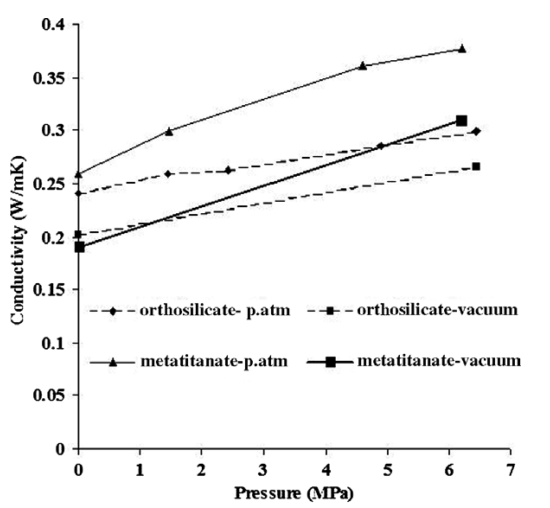
\includegraphics[width=\singleimagewidth]{figures/aquaro.png}
    \caption{Effective conductivity of \lit~and \lis~in air and vacuum environment conditions. Reproduced from Ref \cite{Aquaro2007}.}
    \label{fig:keff-aquaro}
\end{figure}
The solid-solid conductance modeling of DEM can be seen as the vacuum limit when no influence of interstitial purge gas is present; the results of DEM should therefore then be in the range of \SIrange{0.2}{0.3}{\mega\pascal}. 

A recent thermal DEM study has been performed by Gan\etal~which analyzed temperature profiles in pebble bed regions reflecting the European design of helium-cooled pebble bed.\cite{An20072233} In their work, they use the more generic form of heat conductance provided by Batchelor \& O'Brien,\cite{Batchelor1977}
\begin{equation}\label{eq:gan-dem-hc}
H_c = 2\pi\frac{k_s}{\kappa}R^* \mathscr{H}(\kappa,\Psi)
\end{equation}
where $\kappa = k_s/k_g$ as defined above; $\mathscr{H}(\kappa,\Psi)$ is a function of (i) the flux across contact circle, (ii) the difference between the flux across the matrix layer and the total flux between particles in point contact, and (iii) the conductivity ratio $\kappa$. In the limit of $\Psi\rightarrow\infty$ (see \Cref{eq:conductance-validity-fluid}), $\mathscr{H} \rightarrow \frac{\kappa a}{\pi R^*}$ and thus \Cref{eq:batchelor-pebble-conductance} is recovered.

For the case of $\phi = 0.645$, the temperature profile for mono-sized pebbles is reproduced in \Cref{fig:gan-temp-profile-tdem}. 
\begin{figure}[ht]
\centering
    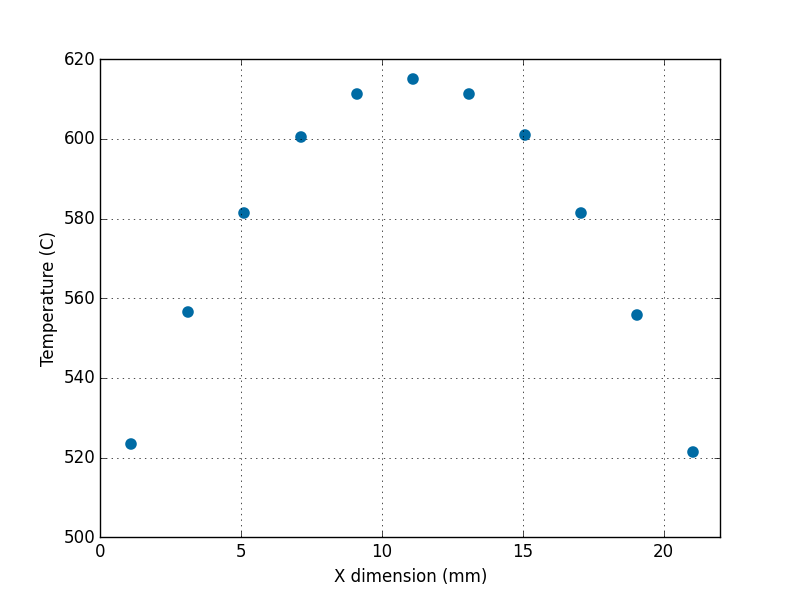
\includegraphics[width=\singleimagewidth]{figures/gan-temp-profile-tdem.png}
    \caption{Temperature profile across a pebble bed from Ref.\cite{An20072233}}
    \label{fig:gan-temp-profile-tdem}
\end{figure}

An effective thermal conductivity can be calculated from the data given by Gan\etal~and using \Cref{eq:keff-formulation}. For the case of $\phi = 0.645$, an effective thermal conductivity is found to be $\keff = \SI{4.37}{\watt\per\meter\per\kelvin}$. In the heat conductance term used by Gan\etal, contribution of helium is accounted for in near-contact regions of pebbles and thus the effective thermal conductivity determined from these beds should be higher than the values of vacuum, yet the value of \SI{4.37}{\watt\per\meter\per\kelvin} is exceedingly high, given the stress state in the pebble bed after heating is calculated as only \SI{5.7}{\mega\pascal}. The effective conductivity was not reported in paper of Gan\etal~and consequently no discussion on why the value is so large is given.

To validate the heat transfer capabilities of our DEM models, a three-dimensional pebble bed consisting of mono-dispersed particles of diameter $d_p$ is analyzed. The particles are constrained by rigid $y$-$z$-planes at locations of $\frac{x}{d_p} = \pm 10$ (the walls of the container). There are periodic boundary conditions in the $y$-direction located at $\frac{y}{d_p} = \pm 5$. Gravity acts in the negative $z$-direction and the particles are resting on a rigid $x$-$y$-plane at $z=0$ (the floor of the container) and held from the top by an $x$-$y$-plane at approximately $\frac{z}{d_p} = 50$ (the roof of the container). The precise height of the container is chosen to satisfy the requested initial packing fraction. Several initial packing fractions are chosen, $\phi_i = $ [59, 61, 62, 64]\% with \num{6875}. The volume is chosen to represent the long, tall, narrow channels seen in many solid breeder module designs\cite{Cho2008, Poitevin2010, Enoeda2003}.

For this study, the material properties were chosen to represent \lit~pebbles, however the thermal properties of \lis~are roughly equal and this validation also applies to pebble beds of that material as well. All the properties come from Ref.~\cite{Gierszewski1998}, though a modified elastic Modulus . They are summarized in Table~\ref{tab:mat-props}

\begin {table}[tp] %

\caption{Material properties used in validation study of $\keff$ for \lit.}
\label {tab:mat-props} \centering %
\begin {tabular}{ cccccc }
\toprule %
E           &     $\nu$     &    k          &    C          &   $\alpha$                \\
(\si{\giga\pascal})     &               & (\si{\watt\per\meter\per\kelvin})         &  (\si{\joule\per\kilogram\per\kelvin})    &   (\si{\per\kelvin})                   \\\toprule
\num{60}           &      \num{0.24}     &  \num{2.4}          &  \num{1156}           &   \num{15e-6}     \\\bottomrule
\end{tabular}
\end{table}

% In the first attempt at packing pebbles into the system, we begin with a common starting point of a filled, lightly packed volume of 10~550 pebbles. We simulate pouring the pebbles into the volume by initializing them into the system from a height of $\frac{z}{d_p} \approx 50$ and allow them to fall under the influence of gravity (see \Cref{fig:fill01}). We pack the pebbles into a higher packing fraction by means of oscillating the walls as if the pebble bed were sitting on a vibrating plate. This was to imitate the vibration packing technique done in our experimental lab when testing pebble beds in the uniaxial compression test stand. The vibration scheme was able to slowly densify the packed bed but, owing to the very small time step of the simulation, the simulation times were impractically large to approach a packing fraction greater than $\phi = 60\%$. 

\begin{figure}[!ht]
    \centering
    \begin{subfigure}[b]{0.25\textwidth}
        \centering
        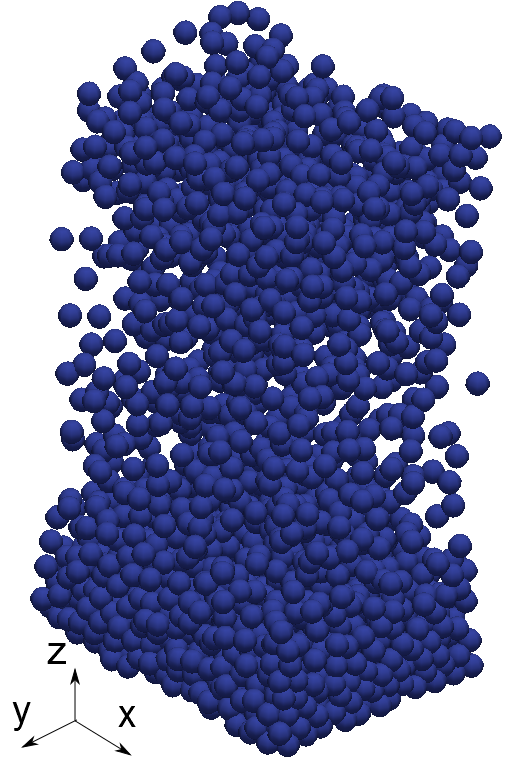
\includegraphics[width=\textwidth]{figures/fill01.png}
    \end{subfigure}
    \begin{subfigure}[b]{0.25\textwidth}
        \centering
        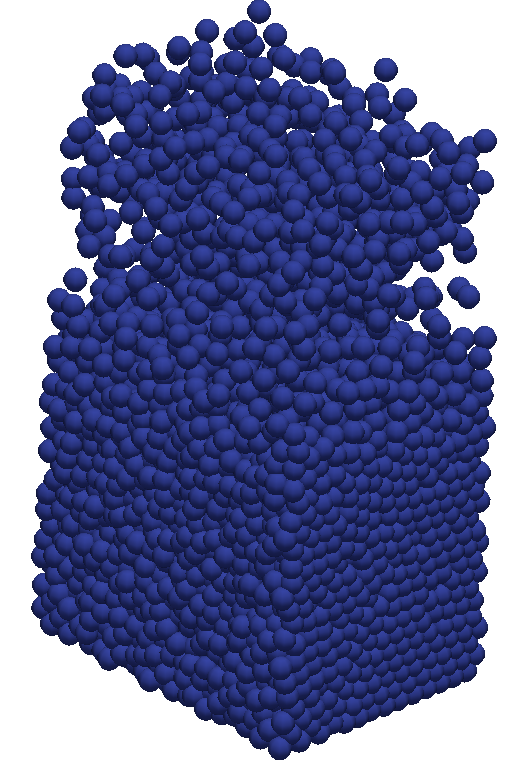
\includegraphics[width=\textwidth]{figures/fill02.png}
    \end{subfigure}
    \begin{subfigure}[b]{0.25\textwidth}
        \centering
        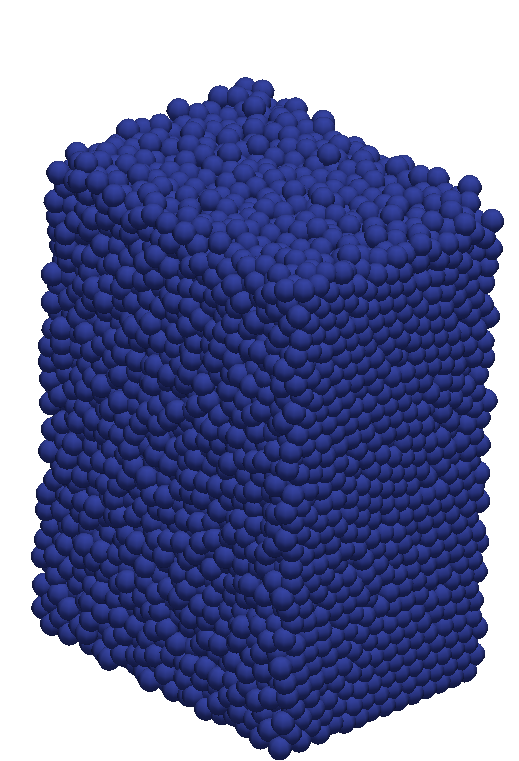
\includegraphics[width=\textwidth]{figures/fill03.png}
    \end{subfigure}
    \caption{Demonstrating the pouring process of pebbles into the control volume with at an early time (left), when it is nearly filled (middle) and after the pebbles have settled to negligible kinetic energy (right).}
\label{fig:fill01}
\end{figure}

The first attempt to pack the bed followed from the `recipes' we had used in physical experiments in the lab. That is, the pebbles were numerically poured into the volume from above and allowed to settle under their own weight (see \Cref{fig:fill01}), then the volume was vibrated while a roof was lowered to compact the system to $\phi = 0.64$, the desired packing fraction. This technique was ultimately abandoned in place of a less realistic but more computationally efficient technique which resulted in comparably packed beds.

In the preferred method, $N$ particles are inserted randomly, with large spacing, into a volume with an expanded $y$-direction. Gravity is not initialized and the coefficient of friction of the pebbles is set to $\mu = 0$. The system boundaries wrapped around the $y$-limits are slowly compressed until they reach the desired volume is obtained (as specified above). In the absence of friction, the pebbles move easily next to each other during the compression and there is no stored tangential forces when the pebble bed is `packed'. Next, the coefficient of friction is increased to a realistic level, $\mu = 0.2$, and gravity in the system is initialized. The bed is then allowed to come to rest, as measured by the kinetic energy of the system. At this point, the pebble bed is considered to be packed and the system state is saved, to be loaded into the heating routine.

%In this first study, we model pebble crushing without considering why the particular pebble should be cracking. In the model we randomly select pebbles from the ensemble, regardless of forces acting upon the pebble, and delete them entirely from the system. When a pebble is removed, the neighboring pebbles react due to the imbalance of forces, and the bed settles into a new configuration. 

To simulate the conditions of a solid breeder in a fusion reactor, where the heat is removed from the pebble bed \textit{via} contact to the containing structure, a constant temperature of $T_\text{c}$ is assigned to the vertical walls. Nuclear heating of the pebbles is simulated through a constant source term on each pebble. A representative heating rate of $Q_s = \frac{q_p'''}{\phi_0}$, where  $q_p'''= 8$ MW/m$^3$ and $\phi_0 = 0.64$.\cite{An20072233} The heating cycle runs until a thermal steady state is reached. Based on a measurement of the total thermal energy of the bed, $E_T =\sum_i^N m_iC_i T_i$, steady-state is determined as $\dt{E_T} = 0$ within a specified tolerance. Once at steady state, effective thermal conductivity of the beds is analyzed for comparison to experimental data on pebbles in vacuum.

Based on the boundary conditions of the system, the heat transfer becomes symmetric and one-dimensional in the $x$-direction from $x=0$ to the walls at $\frac{x}{d_p} = \pm 10$. The pebble bed has negligibly small variation of forces and temperatures in the $y$-direction due to the periodic boundary condition at the edges of the domain. Gravity effects are minor in the overall heat transfer and induce only a slight $z$-dependency to the results. Taking advantage of the pebble bed temperature profile's resemblance to a one-dimensional heat transfer problem to calculate an effective conductivity from an analytic, one-dimensional test case analogy.

Assuming a one-dimensional pebble bed, to find an effective conductivity, we step back into a continuum mechanics formulation where the pebble bed can be represented as a slab of solid material. We can analytically solve for the temperature equation in a slab with heat generation, symmetry about the centerline, and a constant boundary temperature condition.

At steady-state, the temperature of a material with constant temperature boundary conditions ($T(L) = T_s$), constant thermal conductivity ($\keff$), and nuclear heating ($q'''$) obeys the following equation

\begin{equation}\label{eq:continuum-heateqn}
    0 = \frac{\mathrm{d}^2T}{\mathrm{d}x^2} + \frac{q'''}{\keff}
\end{equation}

In nondimensional form, the temperature is
\begin{equation}
    \theta = \frac{T(x) - T_s}{T_0 - T_s}
\end{equation}
where $T_0$ is the temperature at the centerline of this slab (a value found momentarily). The length is nondimensionalized as
\begin{equation}
    x^* = \frac{x}{L}
\end{equation}

Thus \Cref{eq:continuum-heateqn} in nondimensional form is,
\begin{equation}\label{eq:continuum-heateqn-nondim}
    0 = \frac{\mathrm{d}^2\theta}{\mathrm{d}x^{*2}} + G
\end{equation}
where
\begin{equation}
    G = \frac{q'''L^2}{\keff(T_0 - T_s)}
\end{equation}

In the nondimensionalized form, the solution is revealed to be purely geometric,
\begin{equation}\label{eq:continuum-temperature-nondim}
    \theta = 1-x^{*2}
\end{equation}
as $T_0  - T_s = \frac{q'''L^2}{2\keff}$. The nondimensional temperature solution of \Cref{eq:continuum-temperature-nondim} is used to prove the one-dimensional assumption of heat transfer is justified for the pebble beds.


Noting that in this continuum mechanics formulation, we are assuming that the nuclear source, $q'''$ term is applied evenly over the entire volume. In our DEM formulation, our source term applies to a single pebble, $Q_s = \frac{q'''}{\phi}$.% To find the effective thermal conductivity of the `slab' of pebble bed, we must reconcile this discrepency. This is accomplished with the exchange of
% \begin{equation}\label{eq:q-source-translation}
%     q''' = \frac{Q_\text{tot}}{V_\text{tot}} = Q_s \phi_i
% \end{equation}
% where the pebble bed volume is given by the height, $H$, width, $W$, and length, $L$, and $Q_s$ is the source term on each pebble in the DEM ensemble. 

From the solution of \Cref{eq:continuum-heateqn-nondim}, we find the effective conductivity to be
\begin{equation}\label{eq:keff-formulation}
    \keff = \frac{q''' L^2}{2(T_0-T_s)}
\end{equation}

I use this formulation of \Cref{eq:continuum-heateqn-nondim} to analyze and compare the pebble beds.

For our representative pebble bed, after applying the nuclear heating and wall cooling, the steady-state temperature distributions of some representative volumes are given in \Cref{fig:init-packing-temp-dist}. Evident in all three pebble beds, though increasingly so for smaller packing fractions, are loose pebbles that have poor mechanical contact with neighboring pebbles and therefore have arbitrarily high temperatures (the magnitude is only limited by the time of the simulation). We refer to these pebbles as `rattlers'. The phenomena of hot rattlers is possible in DEM simulations because there is no other method of heat removal. This is a strong argument for the need to include helium purge gas in the thermal transport models of ceramic pebble beds. If these hot rattlers persist even in the presence of helium, it could lead to an unfavorable performance of the ceramic solid breeder -- the hot rattlers would sinter and prevent the outgassing of tritium, among other issues. The observation of these isolated pebbles is another motivator for the coupling of DEM to thermo-fluid models. In \Cref{fig:init-packing-temp-dist}, we also see that, intuitively, the more loosely packed the pebble bed, the higher the temperatures.


\begin{figure}[!ht]
    \centering
    \begin{subfigure}[b]{0.2\textwidth}
        \centering
        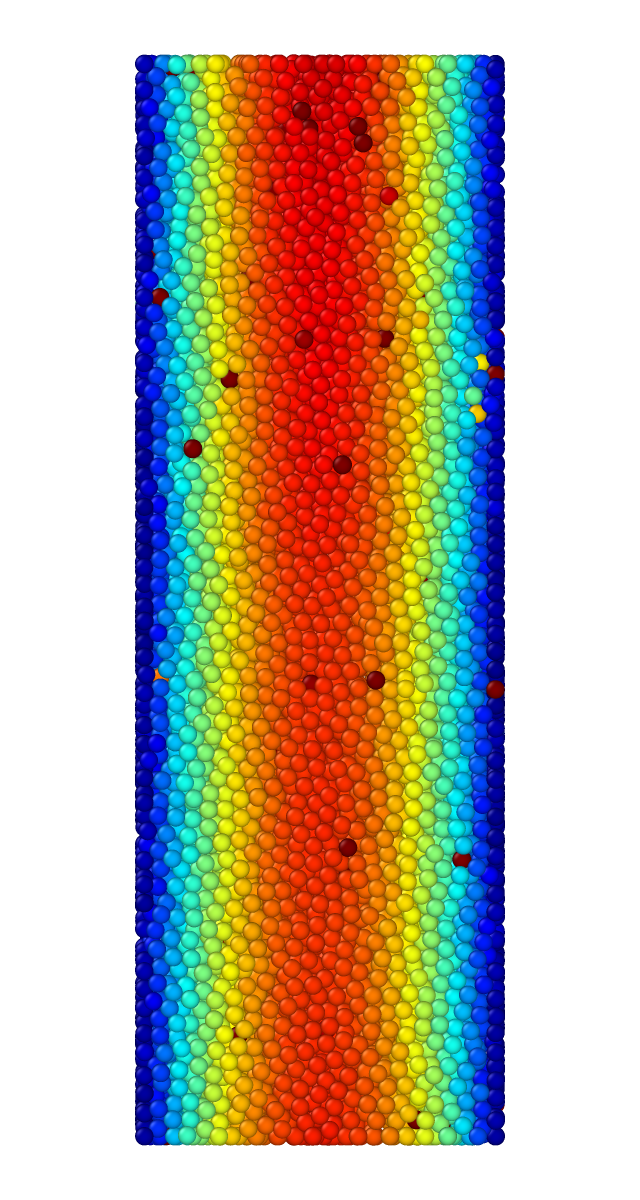
\includegraphics[width=\textwidth]{figures/initial_packing_study/61.png}
        \caption{$\phi_i = 61$\%}
    \end{subfigure}
    ~
    \begin{subfigure}[b]{0.2\textwidth}
        \centering
        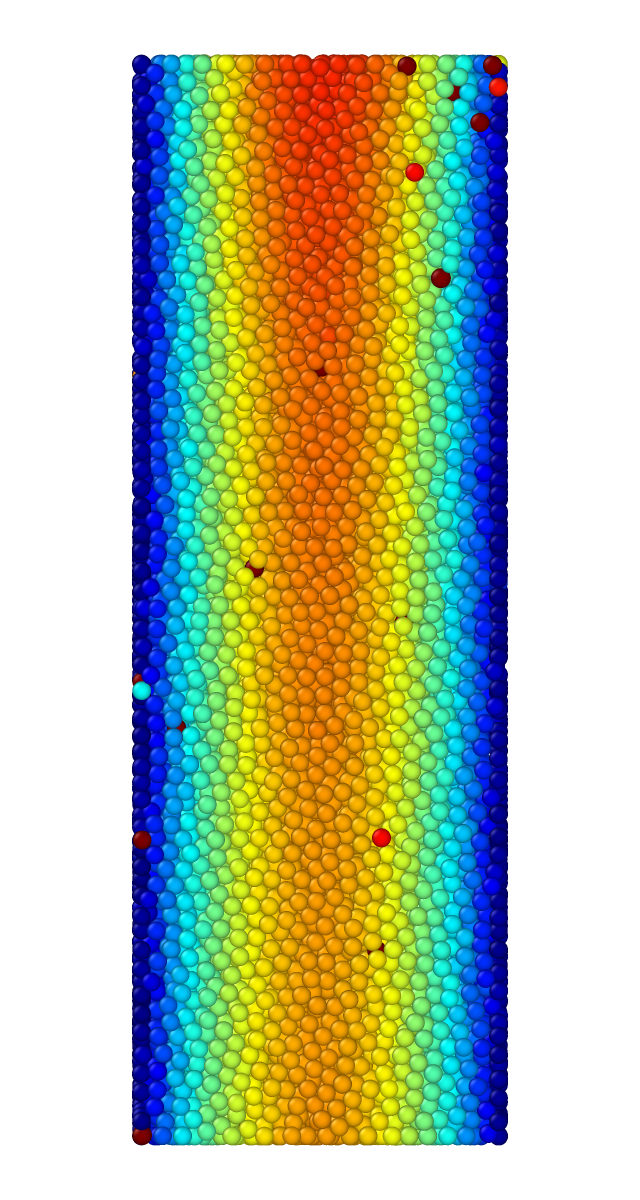
\includegraphics[width=\textwidth]{figures/initial_packing_study/62.png}
        \caption{$\phi_i = 62$\%}
    \end{subfigure}
    ~
    \begin{subfigure}[b]{0.2\textwidth}
        \centering
        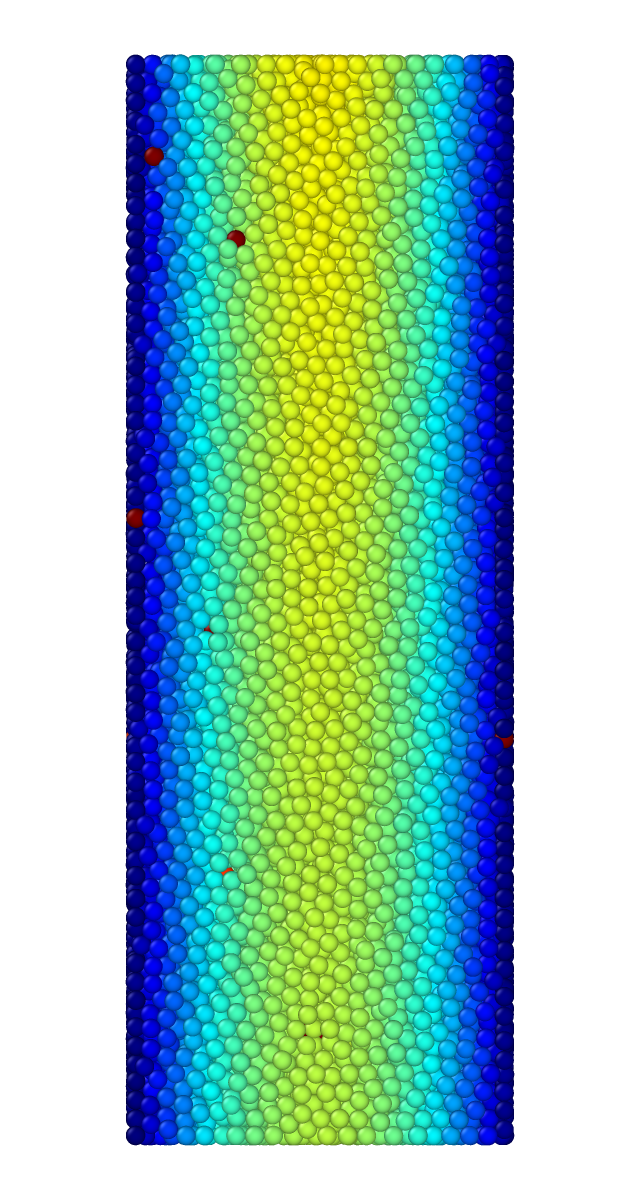
\includegraphics[width=\textwidth]{figures/initial_packing_study/64.png}
        \caption{$\phi_i = 64$\%}
    \end{subfigure}
    
    \begin{subfigure}[b]{0.3\textwidth}
        \centering
        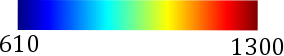
\includegraphics[width=\textwidth]{figures/initial_packing_study/colorbar.png}
    \end{subfigure}
\caption{Temperature distributions in representative packed beds with given initial packing fraction.}
\label{fig:init-packing-temp-dist}
\end{figure}

In order to calculate an effective conductivity of the pebble bed, we find an average temperature profile through the bed. Average values of the bed, along the $x$ direction, are generated \textit{via} averaging temperatures in bins. We create bins that are volumes slices of width $\Delta x$ that extend through the limits of the $y$- and $z$-directions. We then find the $n$ pebbles residing in the slices and take the mean value of their temperatures. The average, given by \Cref{eq:binned-T}, is also shown as the solid lines in \Cref{fig:keff-initial}. The binned average temperature is 
\begin{equation}\label{eq:binned-T}
    \langle T\rangle = \frac{1}{n}\sum_{i}^n T_i    
\end{equation}
Using the volume slices, average contact forces are also found, 
\begin{equation}\label{eq:binned-f}
    \langle F^{1/3} \rangle = \frac{1}{n}\sum_{i}^n F_{n,ij}^{1/3}
\end{equation}


Van Lew\etal~showed that the largest parameter governing the effective conductivity of a granular material like a packed bed is the magnitude of contact forces between pebbles.\cite{VanLew2014} In \Cref{fig:f-ave-initial}, we see the distribution of contact forces as scatter points. The binned average along $x$ is also plotted in the black line. \Cref{fig:f-scatter-59} is given as reference for a pebble bed for which the packing fraction does not completely fill the volume when the pebble bed quiesces. At $\phi_i = 59\%$ there are regions of gap between the top layer of pebbles and the container, as a result the contact forces are on the order of the accumulated weight of the pebbles in the volume. For packing fraction of $\phi_i = 61\%$, we have a relatively well-packed pebble bed with small average contact forces, $\langle F_n \rangle = \SI{5.9}{\newton}$. At an initial packing fraction of $\phi_i = 64\%$, \textit{for the geometry of this bed}, we see somewhat larger average contact forces, $\langle F_n \rangle = \SI{25.9}{\newton}$. In large-volume experiments on pebble beds, such a large contact force would be indicative of being under slight compression and, as such, we expect the effective thermal conductivity of the bed to be larger than the well-packed case of $\phi_i = 61\%$. The effective thermal conductivities are given in the temperature plots of \Cref{fig:keff-initial}.

\begin{figure}[!ht]
    \centering
    \begin{subfigure}[b]{0.45\textwidth}
        \centering
        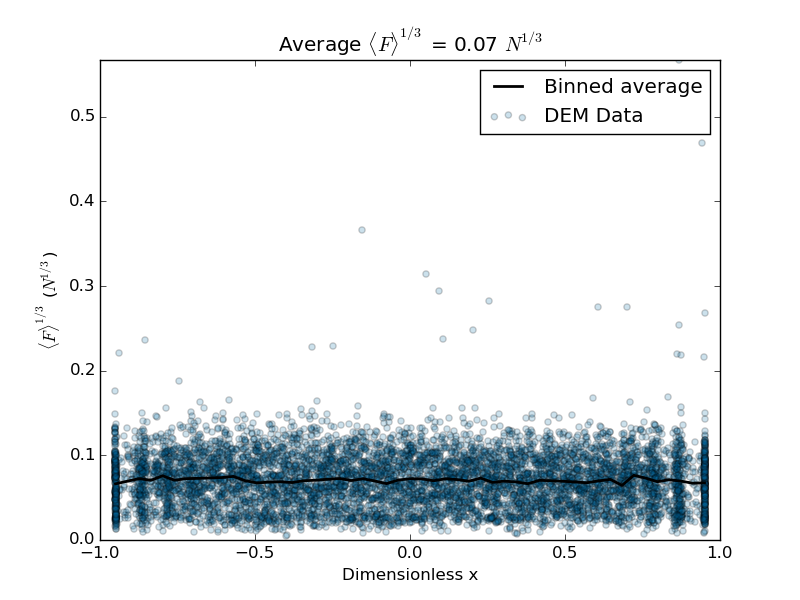
\includegraphics[width=\textwidth]{figures/initial_packing_study/f-scatter-59.png}
        \caption{$\phi_i = 59\%$}\label{fig:f-scatter-59}
    \end{subfigure}
    ~
    \begin{subfigure}[b]{0.45\textwidth}
        \centering
        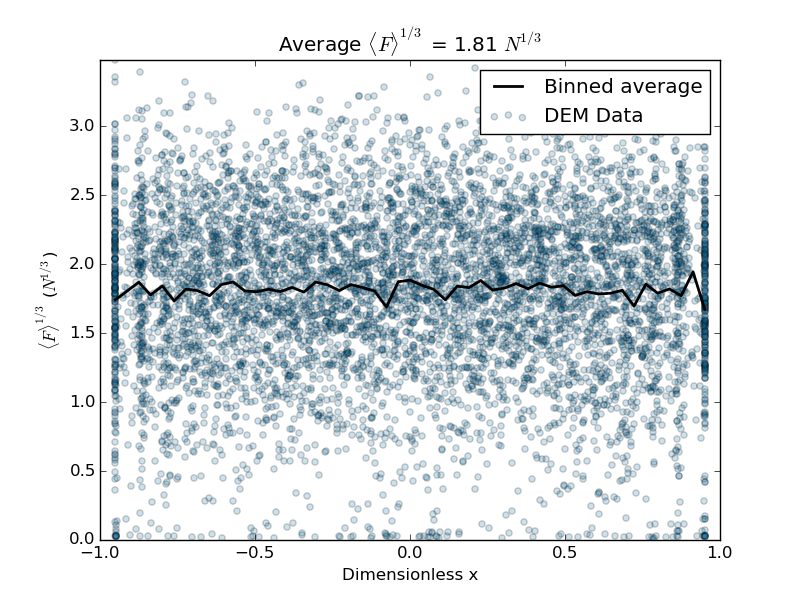
\includegraphics[width=\textwidth]{figures/initial_packing_study/f-scatter-61.png}
        \caption{$\phi_i = 61\%$}
    \end{subfigure}
    
    \begin{subfigure}[b]{0.45\textwidth}
        \centering
        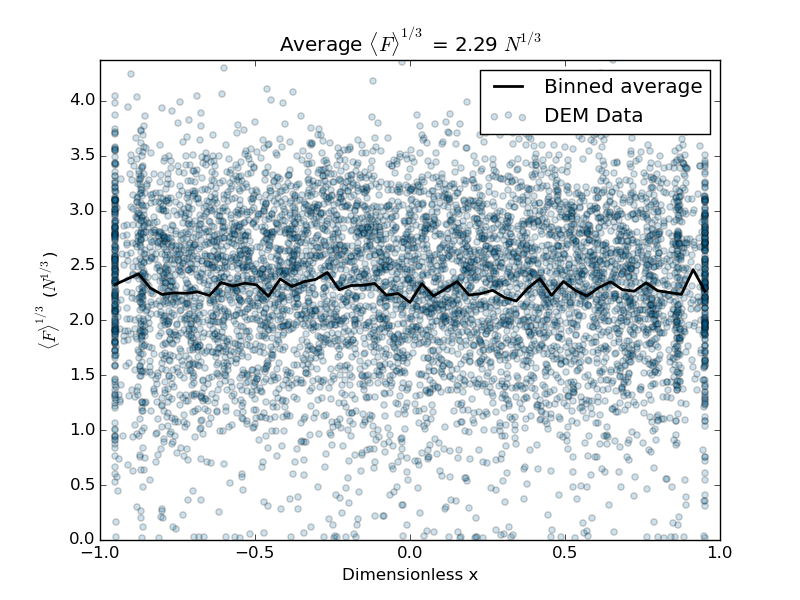
\includegraphics[width=\textwidth]{figures/initial_packing_study/f-scatter-62.png}
        \caption{$\phi_i = 62\%$}
    \end{subfigure}
    ~
    \begin{subfigure}[b]{0.45\textwidth}
        \centering
        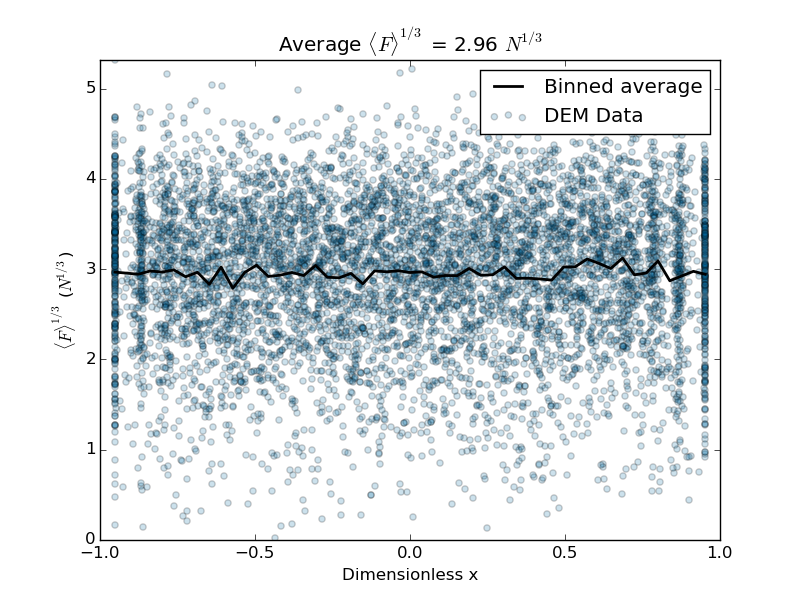
\includegraphics[width=\textwidth]{figures/initial_packing_study/f-scatter-64.png}
        \caption{$\phi_i = 64\%$}
    \end{subfigure}
    \caption{Contact forces in the initially packed beds .}
\label{fig:f-ave-initial}
\end{figure}

\begin{figure}[!ht]
    \centering
    \begin{subfigure}[b]{0.45\textwidth}
        \centering
        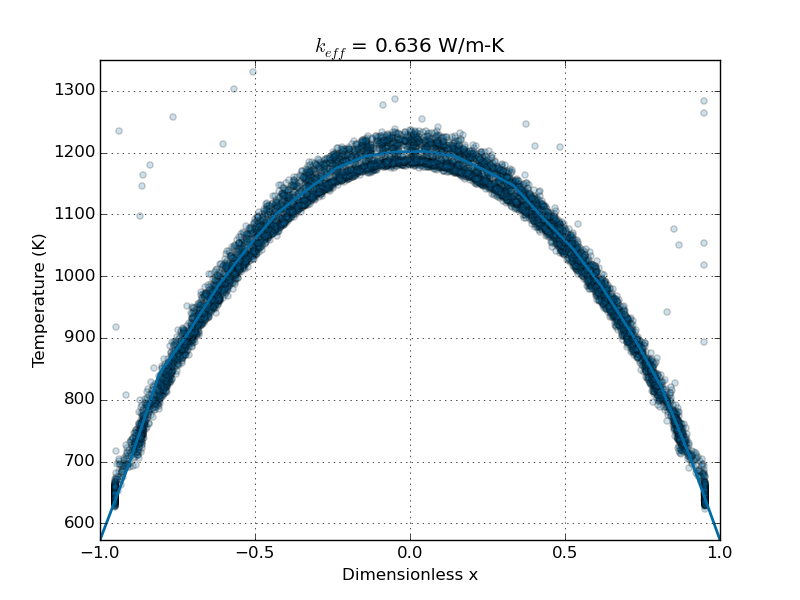
\includegraphics[width=\textwidth]{figures/initial_packing_study/keff-61.png}
        \caption{$\phi_i = 61\%$}
    \end{subfigure}
    ~
    \begin{subfigure}[b]{0.45\textwidth}
        \centering
        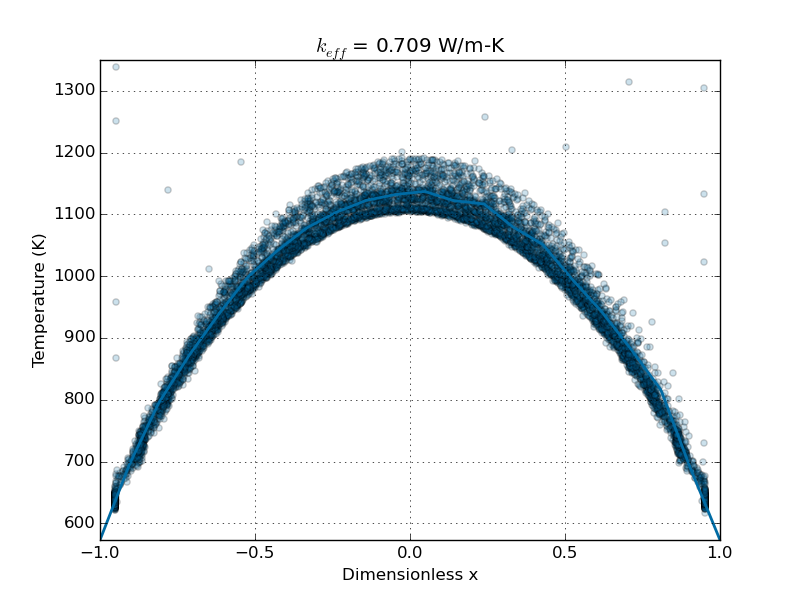
\includegraphics[width=\textwidth]{figures/initial_packing_study/keff-62.png}
        \caption{$\phi_i = 62\%$}
    \end{subfigure}

    \begin{subfigure}[b]{0.45\textwidth}
        \centering
        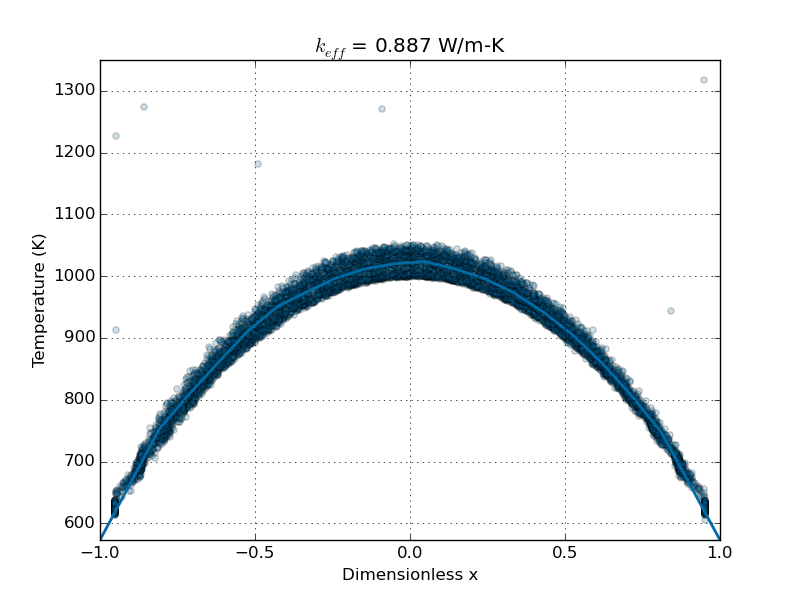
\includegraphics[width=\textwidth]{figures/initial_packing_study/keff-64.png}
        \caption{$\phi_i = 64\%$}
    \end{subfigure}
    \caption{$\keff$ for the packed beds is higher than values measured in experiments in vacuum.}
\label{fig:keff-initial}
\end{figure}

From \Cref{fig:keff-initial}, we see that even the most compliant well-packed bed of case $\phi_i = 0.61$, the effective thermal conductivity is more than three times larger than the measured effective conductivity from experimental data.\cite{ENOEDA} We will see that part of this discrepency is due the current model not accounting for surface roughness of pebble material. For the simulations generating the data of \Cref{fig:keff-initial}, the smooth particle contact conductance model of Batchelor \& O'Brien was used (see \Cref{eq:cheng-modification-batchelor}). In experimental measurements of effective thermal conductivity with roughness, at small loads, effective thermal conductivity of face-centered cubic steel spheroids in an air environment reduced approximately 25\% between cases between a smooth surface ($\sigma = $ \SI{0.03}{\micro\meter}) and rough ($\sigma = $ \SI{1.7}{\micro\meter}).\cite{Buonanno2003a} In spite of the lack of data for roughness of the specific pebbles used in the experiments of Enoeda\etal, we will see that including surface roughness, \textit{via} \Cref{eq:micro-macro-conductance}, allows our DEM models to obtain comparable effective thermal conductivities.

Following ranges of values found in a variety of experimental data,\cite{Bahrami2004} we can choose average parameters for roughness. The asperity height, ranging in experiments from \SIrange{0.12}{13.94}{\micro\meter}; we use an average value of $\sigma = \SI{5}{\micro\meter}$. Vickers hardness is reported for \lit~as $H = 363(1-2.36 \epsilon)$~\si{\mega\pascal}, where $0.1 \le \epsilon \le 0.3$ is the porosity of the bulk ceramic; with $\epsilon = 0.2$, $H = \SI{192}{\mega\pascal}$.\cite{Gierszewski1998,Roux1996a} However, it is unclear if the reported value is the microhardness or macrohardness (as defined by ASTM E384). Surface microhardness can be much larger than bulk hardness.\cite{Bahrami20063691} Regardless, for this study we set the microhardness value equal to $H = \SI{192}{\mega\pascal}$. No Vickers hardness data has been reported for \lis. Using the place-holder roughness values, we use \Cref{eq:micro-macro-conductance} form of conductance to run the above cases again.

Before discussing the results of effective thermal conductivity with roughness, we analyze the effect of the above roughness parameters in order to have an understanding of what to expect in packed beds with rough-surface pebbles. We normalize the heat conductance of \Cref{eq:micro-macro-conductance} by the smooth-sphere conductance of \Cref{eq:cheng-modification-batchelor},
\begin{equation}\label{eq:hjoverhc}
\Gamma = \frac{H_j}{H_c} = \frac{\frac{1}{2k^*a}}{\left(\frac{H'}{E^*\delta_n}\right)^{0.96}\frac{0.031\sigma^{0.598}}{1.720k^*a^{1.04}} + \frac{1}{2k^*a}}
\end{equation}


Therefore we see from \Cref{eq:hjoverhc} that $\Gamma$ is a quantification of reduction in heat conductance due to roughness parameters. Using the a hardness of $H = \SI{15}{\giga\pascal}$, we then find heat conductance reduction, $\Gamma$ as a function of contact force (which determines the value of $a$) and asperity height, $\sigma$. The contour of $\Gamma$ is given in \Cref{fig:roughness-parameters}.

\begin{figure}[ht]
\centering
    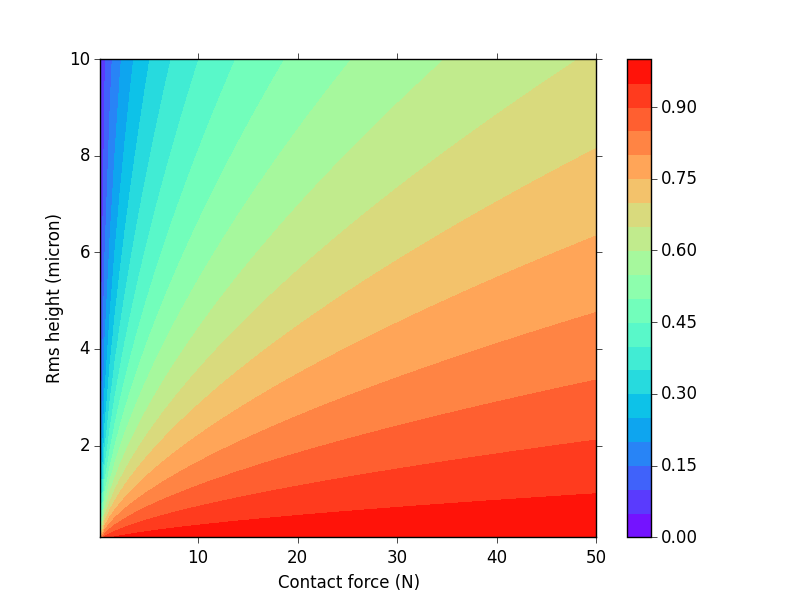
\includegraphics[width=\singleimagewidth]{figures/conductance-contour-roughness.png}
    \caption{Colorbar gives value of $\Gamma$, the measure of reduction in heat conductance comparing calculations with roughness and smooth sphere approximations.}
    \label{fig:roughness-parameters}
\end{figure}

The bed initially packed to $\phi_i = 0.64$, had average contact forces of about \SI{25}{\newton}. According to \Cref{fig:roughness-parameters}, at that force level, with an asperity of \SI{5}{\micro\meter}, contact heat conductance of a rough pebble is 75\% of a similar contact between smooth pebbles. The bed packed to $\phi_i = 0.61$ had average contact forces of \SI{5.9}{\newton}; in this case heat conductance has been reduced approximately 45\% from the smooth approximation. The total effective thermal conductivity is the macroscopic result of heat conductance between all pebbles and can not be linearly extrapolated from heat conductance of any single contact, nonetheless, the measure of $\Gamma$ provides insight into approximate scales of reduction in effective thermal conductivity we should expect when roughness is taken into account.  


Temperature distributions in pebble beds with roughness, along with measures of effective thermal conductivity are given in \Cref{fig:keff-rough-initial}. Accounting for roughness of the pebbles in contact, the effective thermal conductivity of numeric pebble beds approaches the value found in experimental studies of pebble beds in vacuum. When the initial packing fraction is $\phi_i = 0.61$, the effective thermal conductivity falls to $\keff = \SI{0.398}{\watt\per\meter\per\kelvin}$, which compares quite well to experimental measurement of $\keff = \SI{0.2}{\watt\per\meter\per\kelvin}$.


\begin{figure}[ht]
    \centering
    \begin{subfigure}[b]{0.45\textwidth}
        \centering
        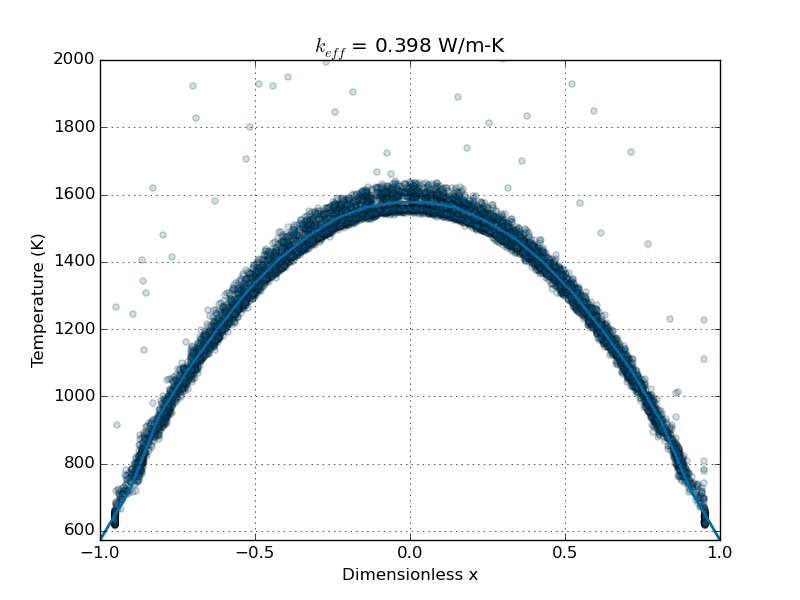
\includegraphics[width=\textwidth]{figures/initial_packing_study/keff-rough-61.png}
        \caption{$\phi_i = 61\%$}
    \end{subfigure}
    ~
    \begin{subfigure}[b]{0.45\textwidth}
        \centering
        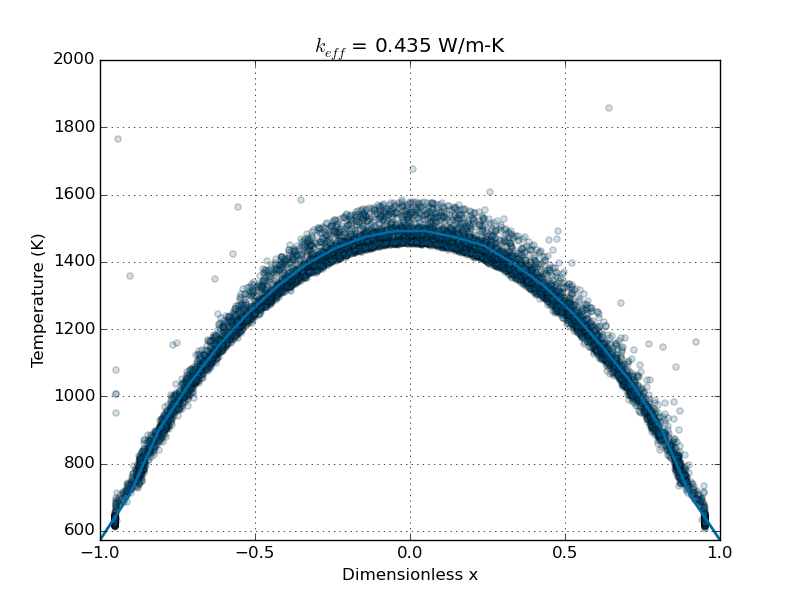
\includegraphics[width=\textwidth]{figures/initial_packing_study/keff-rough-62.png}
        \caption{$\phi_i = 62\%$}
    \end{subfigure}

    \begin{subfigure}[b]{0.45\textwidth}
        \centering
        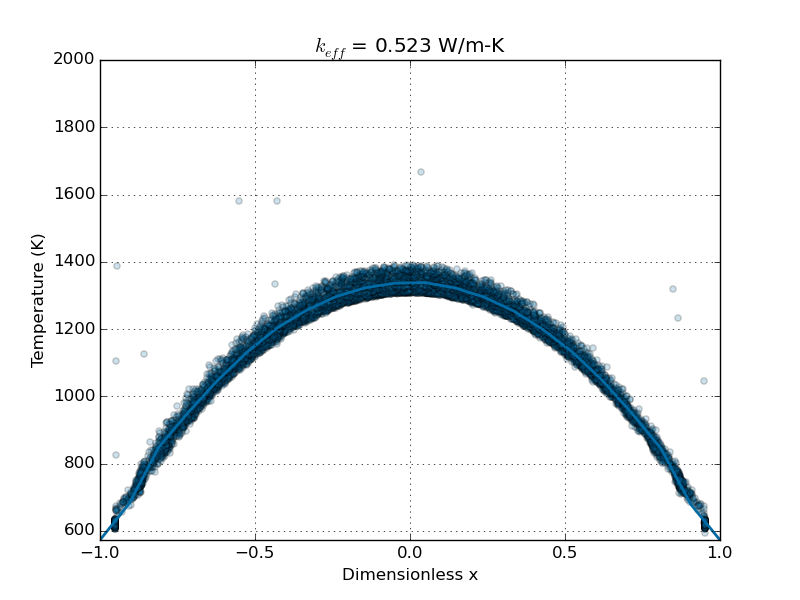
\includegraphics[width=\textwidth]{figures/initial_packing_study/keff-rough-64.png}
        \caption{$\phi_i = 64\%$}
    \end{subfigure}
    \caption{$\keff$ with roughness for given initial packing fractions. Reduced initial packing fractions had lower initial contact forces and therefore effective conductivity values closer to experimentally measured ones.}
\label{fig:keff-rough-initial}
\end{figure}

\FloatBarrier

The effective conductivities of models with the smooth-sphere and roughness approximations are plotted together in \Cref{fig:keff-vacuum-comparisons}. For reference, the grey bar indicates the window of experimental measurements for effective conductivity in vacuum.

\begin{figure}[ht]
\centering
    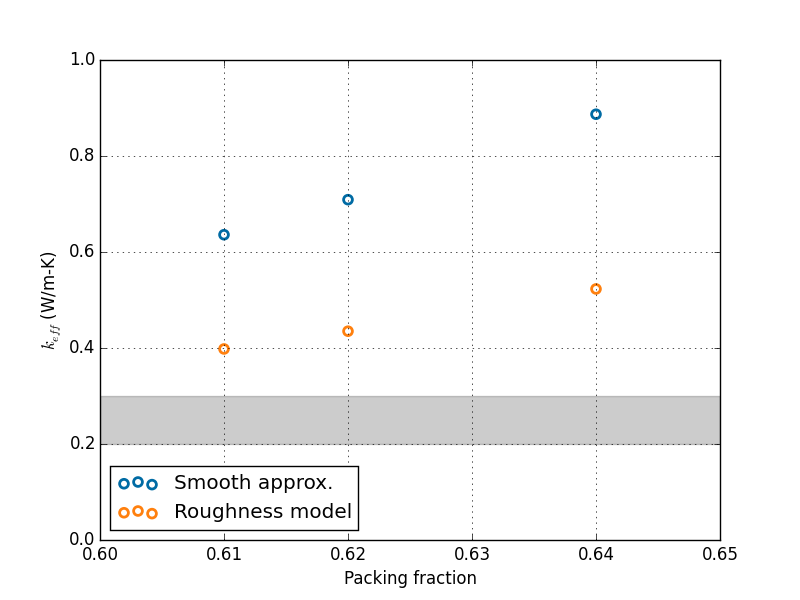
\includegraphics[width=\singleimagewidth]{figures/initial_packing_study/keff-comparisons.png}
    \caption{Comparison of effective conductivity measurements for \lit.}
    \label{fig:keff-vacuum-comparisons}
\end{figure}

The combination of microhardness and asperity height resulted in substantial drops in the effective thermal conductivity of these representative pebble beds. The reductions in effective conductivity were 37\%, 39\%, and 41\% for initial packing fractions of 61\%, 62\%, and 64\%, respectively. While these reductions make the effective conductivity calculated with DEM approach the experimental measurements for pebble beds in vacuum, the values are still more than 25\% higher. The Vicker's microhardness value used in this study could be measured again for other production techniques of lithium ceramics and variations in that value could lead to DEM results that approach even closer to experimental values. Moreover, the arbitrarily-chosen rms asperity height needs to be measured for ceramic pebbles for more accurate roughness contact resistance modeling. Lastly, the majority of ceramic pebbles produced for solid breeders have non-perfect sphericity, some are ovoid or ellipsoidal. However, in the current implementation of DEM, the pebbles are all perfectly spherical. The impact on effective thermal conductivity with geometric variations of the packing material is fertile grounds for future studies.




%%%%%%%%%%%%%%%%%%%%%%%%%%%%%%%%%%%%%%%%%%%%%%%%%%%%%%%%%%%%%%%%%%%%%%%%%%%%%%%%%%%%%%%%%%%%%%%%%%%%%%%%%%%%
%%%%%%%%%%%%%%%%%%%%%%%%%%%%%%%%%%%%%%%%%%%%%%%%%%%%%%%%%%%%%%%%%%%%%%%%%%%%%%%%%%%%%%%%%%%%%%%%%%%%%%%%%%%%
%
% new section
%
%%%%%%%%%%%%%%%%%%%%%%%%%%%%%%%%%%%%%%%%%%%%%%%%%%%%%%%%%%%%%%%%%%%%%%%%%%%%%%%%%%%%%%%%%%%%%%%%%%%%%%%%%%%%
%%%%%%%%%%%%%%%%%%%%%%%%%%%%%%%%%%%%%%%%%%%%%%%%%%%%%%%%%%%%%%%%%%%%%%%%%%%%%%%%%%%%%%%%%%%%%%%%%%%%%%%%%%%%
\section{Elastic Modulus Implementation in DEM for Ceramic Pebbles}\label{sec:exp-reduction-factor}
The discrete element method has been used by many ceramic breeder researchers to model the interaction of individual pebbles in an ensemble.\cite{An20071393, Lu2000, Zhao2010, Gan:2010uq, Annabattula2012a, VanLew2014} In the past studies, the elastic modulus of the ceramic materials used in DEM simulations was taken from historical data, for instance lithium metatitanate from Ref.~\cite{Gierszewski1998}. Furthermore, the assumption of Hertzian descriptions of normal contact for the pebbles is also assumed to be true without direct validation. In our experimental test stand for crushing individual pebbles, shown in \Cref{fig:nfri-fmax}, our equipment was able to record accurate measurements of the force-travel relationship for each pebble. Using the data, we will directly test the validity of Hertzian contact laws for describing interactions of lithium ceramics. 

\begin{figure}[ht]
        \centering
        \begin{subfigure}[b]{\doubleimagewidth}
                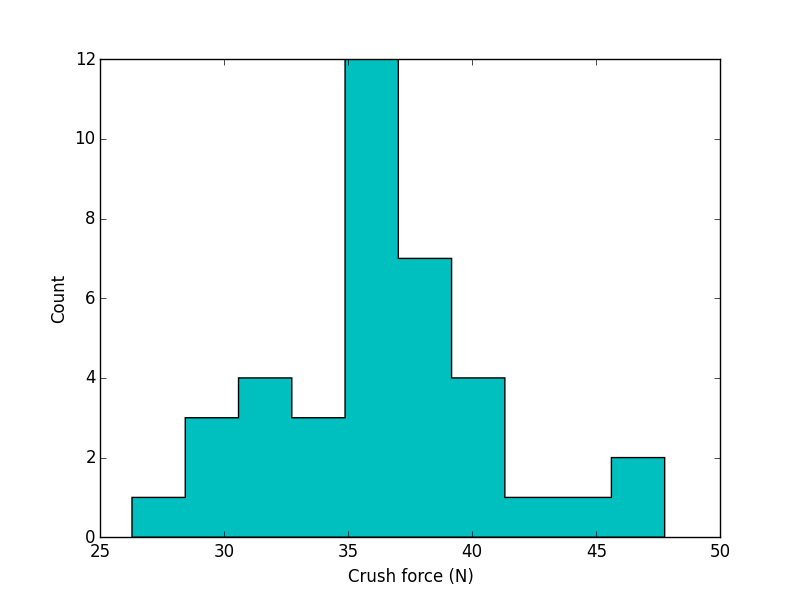
\includegraphics[width=\textwidth]{figures/nfri-1mm-fmax-histogram.png}
                \caption{$\bar{d}_p = 1$ mm}
                \label{fig:nfri-1-exp-fmax}
        \end{subfigure}
        ~
        \begin{subfigure}[b]{\doubleimagewidth}
                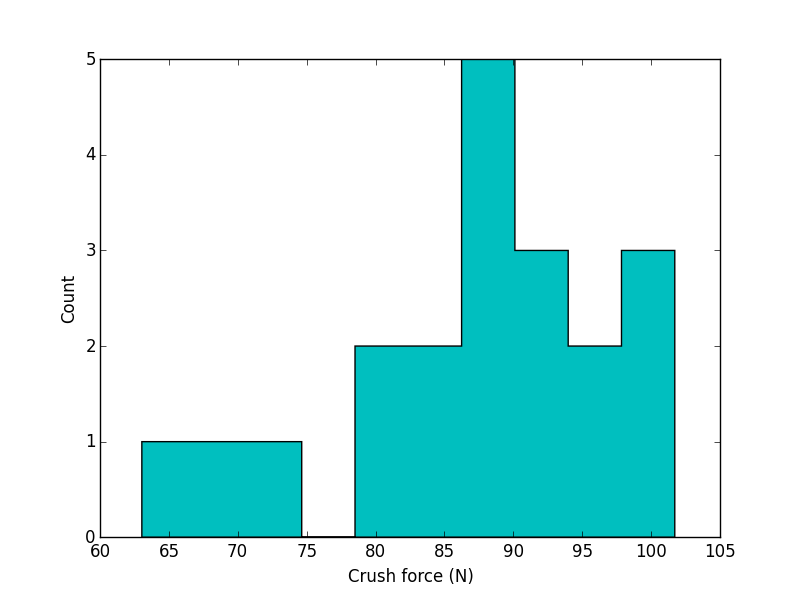
\includegraphics[width=\textwidth]{figures/nfri-1.5mm-fmax-histogram.png}
                \caption{$\bar{d}_p = 1.5$ mm}
                \label{fig:nfri-1.5-exp-fmax}
        \end{subfigure}
        \caption{Crush forces of \lit~pebbles display probability distributions around mean values for each average diameter batch.}\label{fig:nfri-fmax}
\end{figure}

The derivation of the Hertz force can be found on page~\pageref{eq:hertz-normal-force}. The result is given again here for reference:
\begin{equation*}
  F_{n,ij} = \frac{4}{3}E_{ij}^* \sqrt{R_{ij}^*} \, \delta_{n,ij}^{3/2}
\end{equation*}
and, again, the pair elastic modulus and radius are
\begin{align*}
\frac{1}{E^*} & = \frac{1-\nu_i^2}{E_i} + \frac{1-\nu_j^2}{E_j} \\
\frac{1}{R^*} & = \frac{1}{R_i} + \frac{1}{R_j}
\end{align*}

In experiments where we press a ceramic pebble between two anvils, we measure the travel, $s$, of the crosshead rather than the pebble overlap. We modify \Cref{eq:hertz-normal-force} to be represented in terms of travel ($s = 2\delta$). Furthermore, for a pebble ($R_i = R_p$) in contact with a smooth plane ($R_j \rightarrow \infty$), the relative radius is simply $R^* = R_p = d_p/2$. We write the elastic modulus of the pebble as $E_p$ and for the test stand's anvil as $E_s$; similarly for the Poisson ratios of the two materials. The Hertz force acting upon a pebble between anvils is then expressed as a function of the pebble and anvil properties as,
\begin{equation}\label{eq:contact-force}
        F = \left[\frac{1}{3}\frac{\sqrt{d_p}}{\frac{1-\nu_p^2}{E_p} + \frac{1-\nu_s^2}{E_s}}\right] s^{3/2}
\end{equation}

The elastic modulus and Poisson ratio of the test stand are known values that do not vary between pebble experiments. Similarly, in the application of Hertz theory, we also assume the elastic modulus and Poisson ratio of the ceramic are also known and constant. In that case, \textit{for any given pebble diameter}, the term inside the bracket ought to be composed entirely of constants for any given pebble; there would therefore be a single force-travel response possible -- based only on $s$. Using material properties given in Ref.~\cite{Gierszewski1998} for \lit, we plot a set of parametric curves based on diameter over a range of travel. The properties we have used for the nickel-alloy anvil of our test stand and \lit~are given in \Cref{tab:hertz-dp-study-props}. The curves are given in \Cref{fig:hertz-dp-dependence}.

\begin {table}[ht] %
\caption{Material properties used for \lit~and nickel-alloy platen}
\label {tab:hertz-dp-study-props} \centering %
\begin {tabular}{ cccccc }
\toprule %
$E_\text{peb}$      &     $\nu_\text{peb}$  &   $E_\text{stand}$        &     $\nu_\text{stand}$    \\
(GPa)           &                   &   (GPa)               &                   \\\toprule
126             &   0.24                &   220                 &   0.27                \\\bottomrule
\end{tabular}
\end{table}

\begin{figure}[ht]
	\centering
	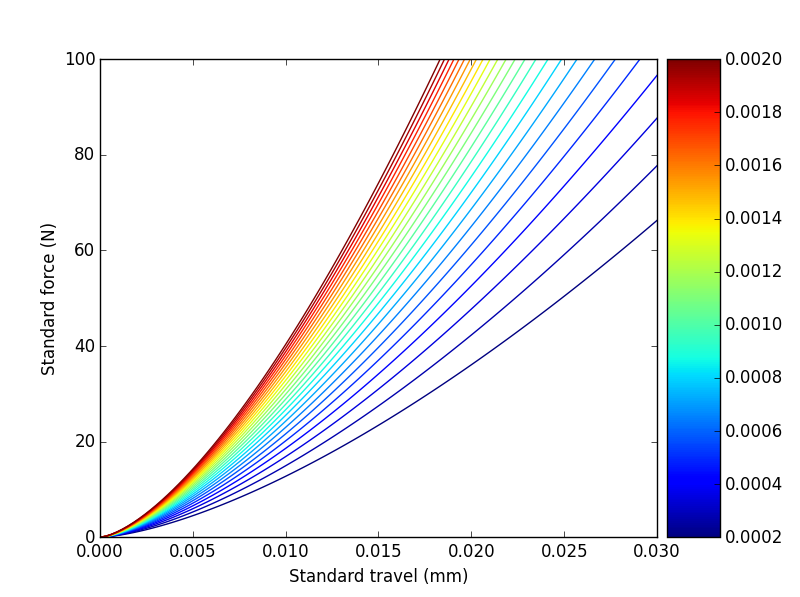
\includegraphics[width = \singleimagewidth]{figures/hertz-dp-dependence}
	\caption{Hertzian responses of \lit~pebbles compressed between platens. The colormap shows pebble diameters in \si{m}. The diameters span an order of magnitude from $d_p = \SI{0.2}{\milli\meter}$ to $d_p = \SI{2}{\milli\meter}$.}\label{fig:hertz-dp-dependence}
\end{figure}

\Cref{fig:hertz-dp-dependence} shows that, for a given pebble, that is strictly obeying Hertz theory, there is only a single force-displacement curve it can follow. However, during our experiments on \lit~pebbles, we observed behavior such as the curves shown in \Cref{fig:nfri-exp-curves}. The diameters of the pebbles are mapped to the colormap on the right side of the figures. These pebbles are responding much different than the expected Hertzian curve, predicted by \Cref{eq:contact-force}. 

We can confirm that the force-travel relationship goes as $F\propto s^{3/2}$ by plotting the force-travel data on log-log plots; the slope of the data represents the power relationship of force and travel. The log-log plots are given in \Cref{fig:nfri-exp-curves-loglog}. The slope of the response is calculated for each experimental curve and a histogram is collected in \Cref{fig:nfri-loglog-slopes}. For both sets of \lit~pebbles, the data is heavily centered around a slope of $n=1.5$, validating the dependence of force on travel as fitting Hertzian predictions.

\begin{figure}[ht]
        \centering
        \begin{subfigure}[b]{\doubleimagewidth}
                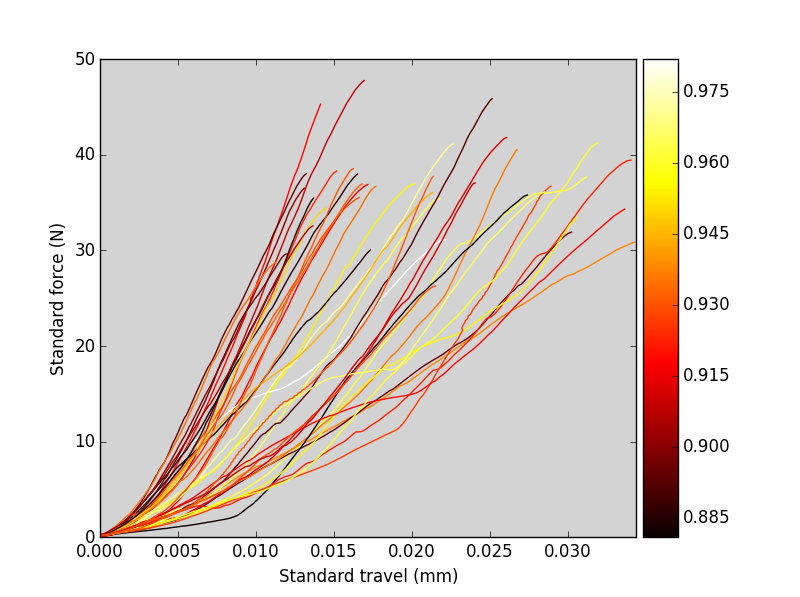
\includegraphics[width=\textwidth]{figures/nfri-1mm-data.png}
                \caption{$\bar{d}_p = 1$ mm}
                \label{fig:nfri-1-exp-colormap}
        \end{subfigure}
        ~
        \begin{subfigure}[b]{\doubleimagewidth}
                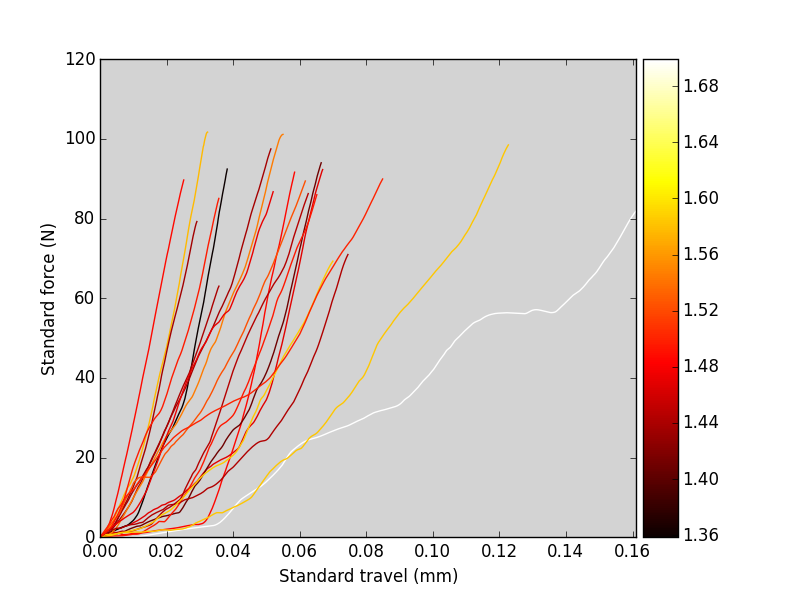
\includegraphics[width=\textwidth]{figures/nfri-1.5mm-data.png}
                \caption{$\bar{d}_p = 1.5$ mm}
                \label{fig:nfri-1.5-exp-colormap}
        \end{subfigure}
        \caption{Experimental measurements of pebble force as a function of cross-head travel.}\label{fig:nfri-exp-curves}
\end{figure}

\begin{figure}[ht]
        \centering
        \begin{subfigure}[b]{\doubleimagewidth}
                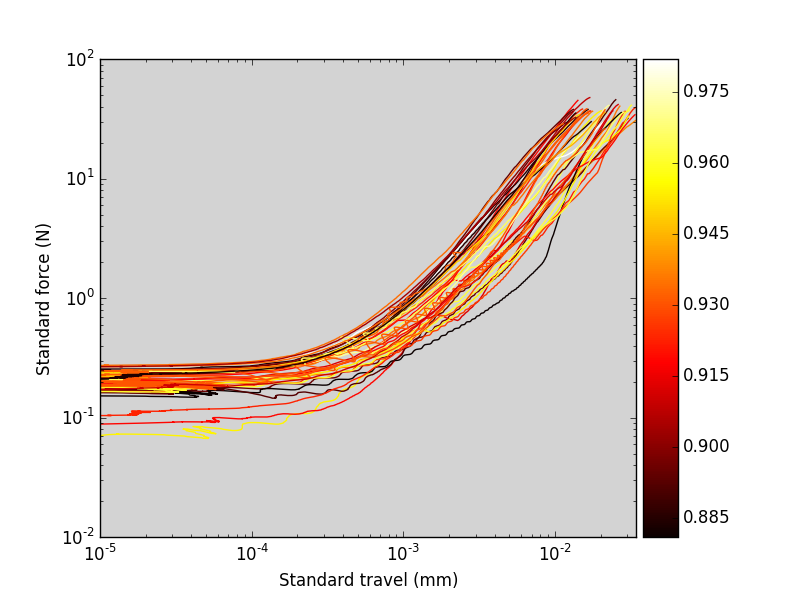
\includegraphics[width=\textwidth]{figures/nfri-1mm-data-loglog.png}
                \caption{$\bar{d}_p = 1$ mm}
                \label{fig:nfri-1-exp-loglog}
        \end{subfigure}
        ~
        \begin{subfigure}[b]{\doubleimagewidth}
                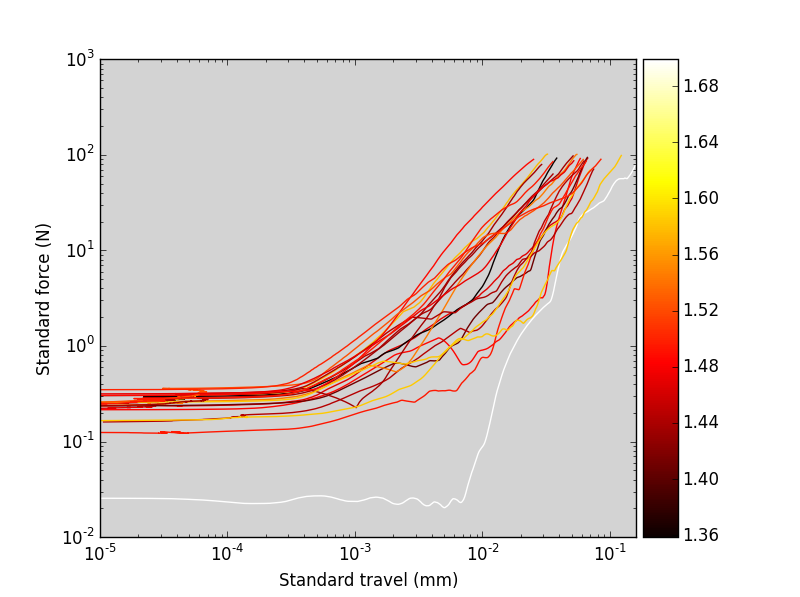
\includegraphics[width=\textwidth]{figures/nfri-1.5mm-data-loglog.png}
                \caption{$\bar{d}_p = 1.5$ mm}
                \label{fig:nfri-1.5-exp-loglog}
        \end{subfigure}
        \caption{Log-log plots of experimental measurements of pebble force as a function of cross-head travel.}\label{fig:nfri-exp-curves-loglog}
\end{figure}

\begin{figure}[ht]
        \centering
        \begin{subfigure}[b]{\doubleimagewidth}
                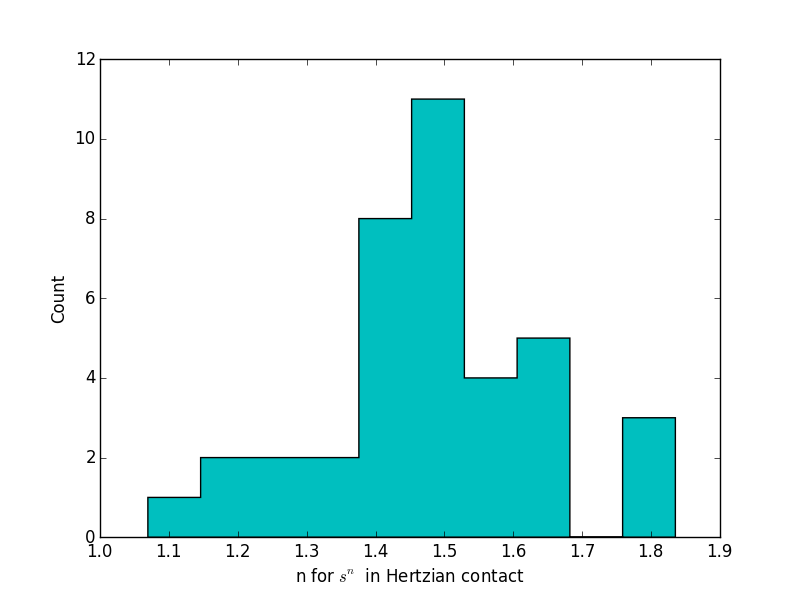
\includegraphics[width=\textwidth]{figures/nfri-1mm-loglog-slope.png}
                \caption{$\bar{d}_p = 1$ mm}
                \label{fig:nfri-1-exp-slope}
        \end{subfigure}
        ~
        \begin{subfigure}[b]{\doubleimagewidth}
                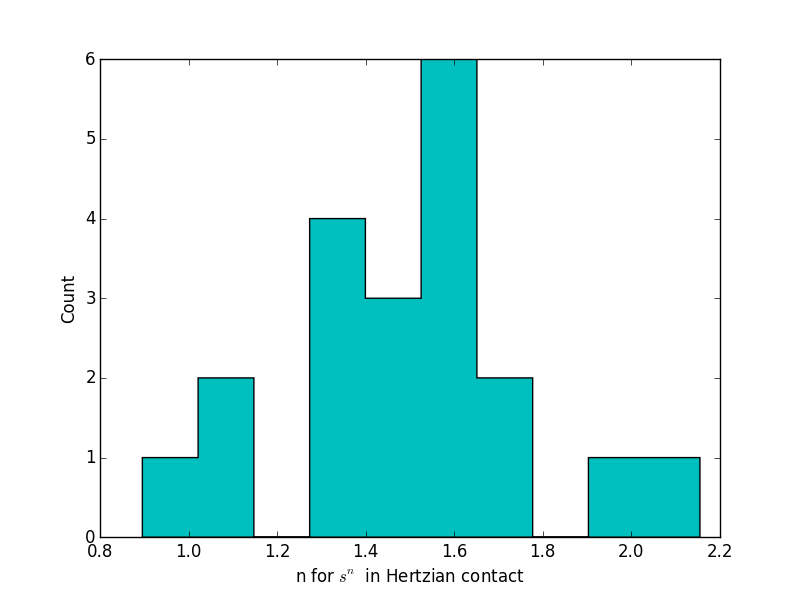
\includegraphics[width=\textwidth]{figures/nfri-1.5mm-loglog-slope.png}
                \caption{$\bar{d}_p = 1.5$ mm}
                \label{fig:nfri-1.5-exp-slope}
        \end{subfigure}
        \caption{Slopes from the log-log plots of experimental measurements of pebble force as a function of cross-head travel show the relation is approximately $F\propto s^{1.5}$.}\label{fig:nfri-loglog-slopes}
\end{figure}

We propose the experimental curves of force travel can be explained \textit{via} unique reductions in elastic modulus of each pebble. We introduce an `apparent' elastic modulus for each pebble which is iteratively found as the elastic modulus which provides the best fit when used in \Cref{eq:contact-force} and compared to force-travel responses from experiments. The apparent elastic modulus is reported normalized against the \lit~elastic modulus from literature, $E_\text{lit}$, 
\begin{equation}
	\kappa = \frac{E_\text{peb}}{E_\text{lit}}
\end{equation}
where we introduce $\kappa$ as a softening coefficient. The sintered pebble value of elastic modulus for \lit~is taken from Ref.\cite{gnielinski1982berechnung} to be $E_\text{lit}= \si{124~GPa}$. Iterating over apparent elastic modulus, the L2-norm of the difference between Hertzian and experimental curves is used as the `error'. The L2 norm, $A$ for a given array, $a$ is 
\begin{equation}
	||A||_F = \left[\sum_{i,j}\textrm{abs}(a_{i,j})^2\right]^{1/2}
\end{equation}

This is a convenient way to compare the error at every point along the force-displacement curves. When the error is minimized, the apparent elastic modulus is recorded and a softening coefficient is calculated. A Hertzian curve (in black), using the apparent elastic modulus in \Cref{eq:contact-force}, is plotted alongside its respective experimental curve in \Cref{fig:nfri-exp-hertz}

\begin{figure}
        \centering
        \begin{subfigure}[b]{\doubleimagewidth}
                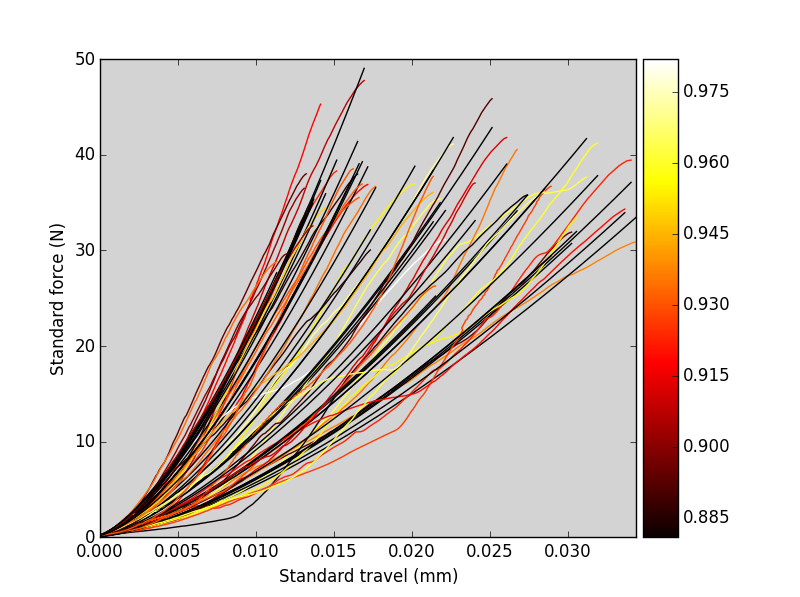
\includegraphics[width=\textwidth]{figures/nfri-1mm-hertz-colormap.png}
                \caption{$\bar{d}_p = 1$ mm}
                \label{fig:nfri-1-exp-hertz}
        \end{subfigure}
        ~
        \begin{subfigure}[b]{\doubleimagewidth}
                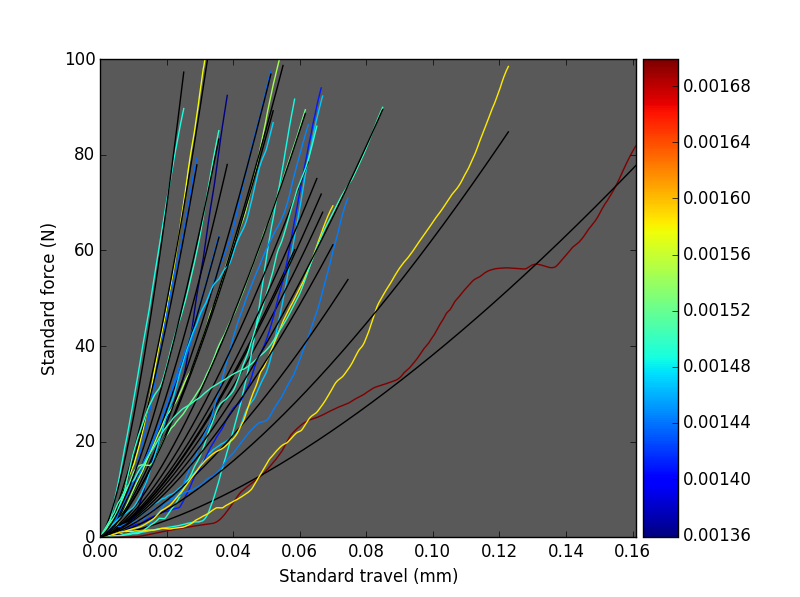
\includegraphics[width=\textwidth]{figures/nfri-1.5mm-hertz-colormap.png}
                \caption{$\bar{d}_p = 1.5$ mm}
                \label{fig:nfri-1.5-exp-hertz}
        \end{subfigure}
        \caption{Force-displacement curves for \lit~pebbles (in color) along with their Hertzian fits (in black) calculated with each pebble having a unique elastic modulus.}\label{fig:nfri-exp-hertz}
\end{figure}

The majority of the curves for two batches of \lit~pebbles analyzed (\Cref{fig:nfri-exp-hertz}) fit well to Hertzian curves with apparent elastic moduli. Apparent elastic moduli of the \lit~pebbles are given in \Cref{fig:nfri-E-plot}. Histograms of $\kappa$ for two batches of \lit~are given in \Cref{fig:nfri-kappa-hist}. The distributions for both batches of \lit~pebbles more closely resemble Snedecor's F distribution with many pebbles behaving with a very small $\kappa$, then a long tail of few pebbles with large $\kappa$.

\begin{figure}
        \centering
        \begin{subfigure}[b]{\doubleimagewidth}
                \includegraphics[width=\textwidth]{figures/nfri-1mm-E-plot.png}
                \caption{$\bar{d}_p = 1$ mm}
                \label{fig:nfri-1mm-E-plot}
        \end{subfigure}
        ~
        \begin{subfigure}[b]{\doubleimagewidth}
                \includegraphics[width=\textwidth]{figures/nfri-1.5mm-E-plot.png}
                \caption{$\bar{d}_p = 1.5$ mm}
                \label{fig:nfri-1.5mm-E-plot}
        \end{subfigure}
        \caption{Distribution of modified elastic modulus for a batch of \lit~pebbles. All pebbles responded to compression with a elastic modulus well below the sintered pellet value of \si{126 GPa}.}\label{fig:nfri-E-plot}
\end{figure}

In \Cref{fig:nfri-kappa-dp-scatter} we see scatter plots of the pebble diameters against $\kappa$ values for the different batches of lithium ceramic pebbles. A Pearson Correlation value was calculated for each of the batches to quantify a correlation between diameter and $\kappa$. For the \lis~pebbles, we find $R = 0.198$ which is a weak positive correlation. For the \lit~pebbles we have $R = -0.385$ for $\bar{d}_p = 1$~mm and $R = -0.201$ for $\bar{d}_p = 1.5$~mm. Both of these are weakly negatively correlated. 

We hypothesize that manufacturing processes of pebbles leads to slightly different internal structures in the ceramic. Those differences yield stronger or weaker pebbles in a probability around a mean value, as seen in \Cref{fig:nfri-1-exp-fmax}. Different internal structure would then also cause each pebble to behave with different stiffness. Thus if the elastic modulus in \Cref{eq:contact-force} for the batch of pebbles had a probability distribution, rather than a single value, we can account for the variations in responses of \Cref{fig:nfri-exp-curves}. 


The results of these single pebble experiments indicate that the elastic modulus traditionally used in DEM simulations for ceramic pebble beds in solid breeders is incorrect. Numerical re-creations of the probability distribution curves will be used to apply $\kappa$ to pebbles in the ensemble. From the weak correlations between diameter and $\kappa$, we are free to ignore any diameter dependence when assigning $\kappa$ values in the DEM framework, especially in light of the current implementation of monodisperse pebble beds. Therefore, numerically, when assigning elastic moduli to the particles in the ensemble, the $\kappa$ distribution will be applied in a random fashion.

% \begin{figure}[ht]
% \centering
%     \includegraphics[width=\doubleimagewidth]{figures/fzk-data-w-ideal-hertz.png}
%     \caption{Dashed lines are \lis~pebbles of approximately \si{0.5 mm} diameter. Solid lines are the Hertzian (Eq.\ref{eq:contact-force}) responses based on each pebble's measured diameter.}
%     \label{fig:fzk-exp-colormap}
% \end{figure}


% \begin{figure}[ht]
% \centering
%     \includegraphics[width=\doubleimagewidth]{figures/fzk-hertz-colormap.png}
%     \caption{Force-displacement curves for \lis~pebbles (in color) along with their Hertzian fits (in black) calculated with each pebble having a unique elastic modulus.}
%     \label{fig:fzk-exp-hertz}
% \end{figure}


% \begin{figure}[ht]
% \centering
%     \includegraphics[width=\doubleimagewidth]{figures/fzk-E-plot.png}
%     \caption{Distribution of modified elastic modulus for a batch of \lis~pebbles. Most pebbles responded to compression with a elastic modulus well below the sintered pellet value of \si{90 GPa}.}
%     \label{fig:fzk-E-plot}
% \end{figure}


% \begin{figure}[ht]
% \centering
%     \includegraphics[width=\doubleimagewidth]{figures/fzk-kappa-histogram.png}
%     \caption{Histogram of $\kappa$ for a batch of \lis~pebbles. Most pebbles responded to compression with a elastic modulus well below the sintered pellet value of \si{90 GPa}.}
%     \label{fig:fzk-kappa-hist}
% \end{figure}

\begin{figure}
        \centering
        \begin{subfigure}[b]{\doubleimagewidth}
                \includegraphics[width=\textwidth]{figures/nfri-1mm-kappa-histogram.png}
                \caption{$\bar{d}_p = 1$ mm}
                \label{fig:nfri-1mm-kappa-hist}
        \end{subfigure}
        ~
        \begin{subfigure}[b]{\doubleimagewidth}
                \includegraphics[width=\textwidth]{figures/nfri-1.5mm-kappa-histogram.png}
                \caption{$\bar{d}_p = 1.5$ mm}
                \label{fig:nfri-1.5mm-kappa-hist}
        \end{subfigure}
        \caption{Histogram of $\kappa$ for two batches of \lit~pebbles. All pebbles responded to compression with a elastic modulus well below the sintered pellet value of \si{126 GPa}.}\label{fig:nfri-kappa-hist}
\end{figure}


% \begin{figure}[!ht]
% \centering
%     \includegraphics[width=\doubleimagewidth]{figures/fzk-kappa-dp-scatter.png}
%     \caption{Scatter of $\kappa$ against pebble diameter for a batch of \lis~pebbles showing almost no relationship between apparent stiffness and diameter.}
%     \label{fig:fzk-kappa-dp-scatter}
% \end{figure}

\begin{figure}
        \centering
        \begin{subfigure}[b]{\doubleimagewidth}
                \includegraphics[width=\textwidth]{figures/nfri-1mm-kappa-dp-scatter.png}
                \caption{$\bar{d}_p = 1$ mm}
                \label{fig:nfri-1mm-kappa-dp-scatter}
        \end{subfigure}
        ~
        \begin{subfigure}[b]{\doubleimagewidth}
                \includegraphics[width=\textwidth]{figures/nfri-1.5mm-kappa-dp-scatter.png}
                \caption{$\bar{d}_p = 1.5$ mm}
                \label{fig:nfri-1.5mm-kappa-dp-scatter}
        \end{subfigure}
        \caption{Scatter of $\kappa$ against pebble diameter for two batches of \lit~pebbles showing almost no relationship between apparent stiffness and diameter.}\label{fig:nfri-kappa-dp-scatter}
\end{figure}

\FloatBarrier


%~~~~~~~~~~~~~~~~~~~~~~~~~~~~~~~~~~~~~~~~~~~~~~~~~~~~~~~~~~~~~~~~~~~~~~~~~~~~~~~~~~~~~~~~~~~~~~~~~~~~~~~~~~~
% new subsection
%~~~~~~~~~~~~~~~~~~~~~~~~~~~~~~~~~~~~~~~~~~~~~~~~~~~~~~~~~~~~~~~~~~~~~~~~~~~~~~~~~~~~~~~~~~~~~~~~~~~~~~~~~~~
\subsection{Elastic Modulus Influence on Mechanical Response of Pebble Beds}\label{sec:dem-studies-youngs-modulus}

Proper calculation of normal force in DEM simulations is critical for accuracy in heat transfer modeling, as seen in \Cref{eq:cheng-modification-batchelor}, as well as accuracy in predictions of pebble crushing, as will be shown in \Cref{sec:failure-study}. We showed in the previous section that Hertzian contact is generally valid for describing pebble interactions. The Hertzian force is linearly proportional to the pair elastic modulus of contacting spheres. Based on the softening coefficient, $\kappa$, values found in \Cref{sec:exp-reduction-factor}, the apparent elastic moduli of \lis~and \lit~are, on average, less than half the values given for sintered materials in literature. For the case of \lit, the average value was closer to only 10\% of the value from literature. Thus the actual contact forces in pebble beds may be 10\% of the values found from DEM simulations with incorrect elastic modulus! In this section, we compare a number of pebble beds modeled with DEM using different elastic moduli. 

We first simulate uniaxial compression tests on pebble beds. One set of beds will be composed of pebbles with the single elastic modulus from literature and the other set will be composed of pebbles with a distribution of elastic moduli that fit the distribution from experiments. The second set of numerical experiments will simply compare the effective thermal conductivity of pebble beds as a function of elastic modulus.
%~~~~~~~~~~~~~~~~~~~~~~~~~~~~~~~~~~~~~~~~~~~~~~~~~~~~~~~~~~~~~~~


\subsubsection{Uniaxial Compression Simulations: Numerical Setup}
%In pebble bed breeder units, the stresses on the pebble regions are a result of thermal expansion of the relatively hot pebbles contained by relatively cool container walls. This process is a function of the coefficient of thermal expansion of the pebbles and their elevated temperature; the confined strain relates to a stress. 
The pebble beds are modeled as undergoing a standard uniaxial compression up to 6 MPa while measuring the macroscopic stress-strain for some parametrically varied pebble beds. At the moment of maximum stress, we can investigate the differences in contact forces of the different pebble beds.

Our pebble ensemble is composed of \SI{0.5}{\milli\meter} diameter \lis~pebbles. The pebble beds are initiated and packed in the same manner as \Cref{sec:dem-benchmark}. There are two main bed groups. Set A: three beds (A.1-3) containing a single type of pebble with $E$ = \si{90 GPa}. Set B: four beds (B.1-4) containing ten types of pebbles with their elastic modulus assigned in a discrete, random way to satisfy the distribution seen from experimental data. For the DEM study, \lis~pebbles are fit with a Weibull distribution of shape parameter $\sigma = 1.6$ where the average stiffness was $\bar{E} = 49$~GPa. The description of the two sets of pebble beds is visually represented in \Cref{fig:dem-types}. The pebble bed geometry was also the same used in the study of Ref.~\cite{VanLew2014}~: two virtual walls in the x-direction located at $x_\text{lim} = \pm 20 R_p$, periodic boundaries at the limits of $y_\text{lim} = \pm 15 R_p$, and a total of 8000 pebbles packed into the volume to an approximate height of $z_\text{lim} = 20 R_p$.

Among both sets, a parametric study was done on pebble radius and coefficient of friction. The radii of pebbles in beds A.1, A.2, B.1, and B.2 were constant at $R_p$=.25 mm. The radii of pebbles in beds A.3, B.3, and B.4 followed a Gaussian distribution about $\bar{R}_p$ = 0.25 mm: $\mu_d = R_p$ and $\sigma_d = R_p$. The coefficient of friction was set at $\mu = 0.2$ for beds A.1, A.3, B.1, and B.3; the coefficient of friction was $\mu = 0.3$ for beds A.2, B.2, and B.4.


\begin{figure}[t]
  \centering
  \includegraphics[width=\singleimagewidth]{figures/DEM-types}
  \caption{On the left, set A, a pebble bed with a single type, of $E = 120$ GPa. On the right, set B, is a pebble bed with 10, randomly distributed types; each type corresponds to a reduced, apparent elastic modulus as derived from experimental data.}\label{fig:dem-types}
\end{figure}



%~~~~~~~~~~~~~~~~~~~~~~~~~~~~~~~~~~~~~~~~~~~~~~~~~~~~~~~~~~~~~~~
\subsubsection{Uniaxial Compression Simulations: Results}


A constant-velocity, uniaxial compression was applied to the pebble beds. A single cycle up to \SI{6}{\mega\pascal} then down to \SI{0}{\mega\pascal} was used on all the beds. The macroscopic measurements of stress-strain are shown for all the pebble beds in \Cref{fig:stress-strain}.

\begin{figure}[t]
  \centering
  \includegraphics[width=\singleimagewidth]{figures/stress-strain}
  \caption{Stress-strain responses of pebble beds with: squares, constant elastic modulus; and circles, Gaussian distribution of elastic modulus. The constant elastic modulus beds all had much firmer responses for all parametric cases studied here.}\label{fig:stress-strain}
\end{figure}

Naturally, the pebble beds with smaller elastic�s modulus (with circle markers) are more compliant to external loads. The result is true regardless of the coefficient of friction or distribution of pebble radius studied here. Group B moved to an average strain of about 2.6\% at \SI{6}{\mega\pascal}, by comparison the beds of Group A only had strained 1.9\% on average to reach the same stress. Among the beds of each group, pebble beds with constant radius pebbles behaved virtually the same as similar pebble beds with a Gaussian distribution on radius. An increase in the coefficient of friction had a moderate impact on the overall stress-strain response. 


The parametric study here shows that the largest contributor to stress-strain response is the elastic�s modulus. The coefficient of friction and radius distribution had comparatively insignificant influence. A pebble bed geometry more directly comparable to oedometric compression experiments should be used to allow direct comparison and validation of the numerical models.


At the point of peak stress for each bed, DEM results are used to visualize the distribution of contact forces among all pebbles in the ensemble. A plot of the probability distributions of all the beds together, \Cref{fig:all-contact-forces}, shows that the majority of the contacts in all the beds are equally small. There are a few overall trends we observe from the results however. The pebble beds with the constant elastic modulus are always higher for their comparable version with distributed elastic modulus. For pebble beds with comparable elastic moduli and radii, higher coefficients of friction generally have higher peak contact forces. Pebble beds' radius distributions have much less impact on peak contact forces than either coefficient of friction or elastic�s modulus. Another method of comparing overall contact force distributions is to consider predictions on pebble cracking which assigns a strength value at random to pebbles in the bed (details are given in \Cref{sec:exp-reduction-factor}). At the point of maximum stress, this is done and the results are shown in \Cref{tab:num-crush-percent}.

While overall the predicted number of broken pebbles is small, we compare similar parameteric pebble beds and in each case pebble beds with modified elastic�s modulus overall predict smaller percentages of broken pebbles. Pebble crushing is a major topic for the overall evaluation of the feasibility of ceramic pebble beds in fusion reactors. This study reveals that past DEM work on pebble crushing, such as Ref.~\cite{Annabattula2012a,Annabattula2014,Zhao2013}, were likely over-predicting the extent of crushing if the elastic modulus used in the study was much larger than the realistic response of individual pebbles.

\begin{figure}[t]
  \centering
  \includegraphics[width=\singleimagewidth]{figures/all-contact-forces}
  \caption{Probability distribution of contact forces in all the pebble beds studied here. Elastic moduli value is the largest contributor to higher peak contact forces among pebbles.}\label{fig:all-contact-forces}
\end{figure}


\begin{table}[t]
\caption{Comparisons for the two styles of elastic moduli used in the study. }
\label{tab:num-crush-percent}
\centering
\resizebox{0.45\textwidth}{!}{
\begin{tabular}{llS[table-format=3.2]}
\toprule
Bed label		& 		Parameters 								&	\text{Predicted crushed}			\\
				& 												&	\multicolumn{1}{r}{\text{\%}}		\\\otoprule
A.1				& 		$E$, $R_p$, $\mu = 0.2$          		&	0.3									\\\midrule
A.2				& 		$E$, $R_p$, $\mu = 0.3$     			&	1.0									\\\midrule
A.3				& 		$E$, $\bar{R}_p$, $\mu = 0.2$			&	0.9									\\\midrule
B.1				& 		$\bar{E}$, $R_p$, $\mu = 0.2$			&	0.6									\\\midrule
B.2				& 		$\bar{E}$, $R_p$, $\mu = 0.3$			&	0.8									\\\midrule
B.3				& 		$\bar{E}$, $\bar{R}_p$, $\mu = 0.2$		&	0.4									\\\midrule
B.4				& 		$\bar{E}$, $\bar{R}_p$, $\mu = 0.3$		&	0.7									\\\bottomrule
\end{tabular}}
\end{table}



% \subsubsection{elastic Modulus Influence on Heat Transfer: Numerical Setup}
% \subsubsection{elastic Modulus Influence on Heat Transfer: Results}



%~~~~~~~~~~~~~~~~~~~~~~~~~~~~~~~~~~~~~~~~~~~~~~~~~~~~~~~~~~~~~~~~~~~~~~~~~~~~~~~~~~~~~~~~~~~~~~~~~~~~~~~~~~~
% new subsection
%~~~~~~~~~~~~~~~~~~~~~~~~~~~~~~~~~~~~~~~~~~~~~~~~~~~~~~~~~~~~~~~~~~~~~~~~~~~~~~~~~~~~~~~~~~~~~~~~~~~~~~~~~~~
% \subsection{Conclusions of elastic Modulus Study}










\FloatBarrier

%%%%%%%%%%%%%%%%%%%%%%%%%%%%%%%%%%%%%%%%%%%%%%%%%%%%%%%%%%%%%%%%%%%%%%%%%%%%%%%%%%%%%%%%%%%%%%%%%%%%%%%%%%%%
%%%%%%%%%%%%%%%%%%%%%%%%%%%%%%%%%%%%%%%%%%%%%%%%%%%%%%%%%%%%%%%%%%%%%%%%%%%%%%%%%%%%%%%%%%%%%%%%%%%%%%%%%%%%
%
% new section
%
%%%%%%%%%%%%%%%%%%%%%%%%%%%%%%%%%%%%%%%%%%%%%%%%%%%%%%%%%%%%%%%%%%%%%%%%%%%%%%%%%%%%%%%%%%%%%%%%%%%%%%%%%%%%
%%%%%%%%%%%%%%%%%%%%%%%%%%%%%%%%%%%%%%%%%%%%%%%%%%%%%%%%%%%%%%%%%%%%%%%%%%%%%%%%%%%%%%%%%%%%%%%%%%%%%%%%%%%%
\section{Pebble Damage Modeling}\label{sec:failure-study}

To address pebble damage, there are two major modeling tasks: (i) predictive models for pebble crush events and (ii) modeling fragmentation after a crush event. For (i), the task is to develop a model to relate inter-particle pebble forces in an ensemble to measured crush loads of pebbles from experiments. Appendix \Cref{sec:pebble-crush-prediction} discusses predictive models developed in the fusion community as well as other theory behind a predictive model developed recently at UCLA. To address (ii), models must exist which simulate damage pebbles; \textit{i.e.} a scheme to treat a cracked, shattered, or crushed pebble in the assembly as small particles, removed particles, or particles with modified material properties.

Modeling of `crushed pebbles' in numerical assemblies has been attempted by a number of researchers. In most cases, indirect changes to the simulation are done with the hope of matching macroscopic features of beds that are observable in assemblies with damaged pebbles. In work by Marketos and Bolton, they treated a crushed pebble very similar to Van Lew\etal; when a pebble was damaged it was removed completely from the assembly.\cite{Marketos2007,VanLew2014} Marketos and Bolton study the stress-strain response of a pebble bed with a predictive crushing routine while Van Lew\etal~studied the effective thermal conductivity of a damaged pebble bed.

Annabattula\etal, noting the computationally expensive approach of modeling small fragments, introduced damaged pebbles \textit{via} reduction in elastic modulus.\cite{Annabattula2012a} Annabattula\etal~was also interested in the mechanics of the pebble bed with the presence of crushable materials. The study highlighted the differences in behavior of assemblies with different failure criteria and initial packings. From \Cref{fig:annabattula-stress-strain}, results are qualitatively similar to the stress-strain curves depicted by Marketos\etal.

\begin{figure}[ht]
\centering
	\includegraphics[width=\singleimagewidth]{figures/markets-bolton-stress-strain-crushing.jpg}
	\caption{Stress-strain response of a pebble bed with crushed pebbles modeled with removal of pebbles from assembly. Reproduced from Ref.~\cite{Marketos2007}}
	\label{fig:marketos-bolton-stress-strain}
\end{figure}

\begin{figure}[ht]
\centering
	\includegraphics[width=\singleimagewidth]{figures/annabattula-stress-strain-crushing.jpg}
	\caption{Stress-strain response of a pebble bed with crushed pebbles modeled with reduction in elastic modulus with varying failure criteria. Reproduced from Ref.~\cite{Annabattula2012a}}
	\label{fig:annabattula-stress-strain}
\end{figure}


\begin{figure}[ht]
\centering
	\includegraphics[width=\singleimagewidth]{figures/ben-nun-configurations}
	\caption{Configurations of fragmentation used in the study of Ref.~\cite{Ben-Nun2010a}}
	\label{fig:ben-nun-configurations}
\end{figure}


Ben-Nun\etal~studied the effects of fragmentation in two dimensional DEM studies of compressed packings.\cite{Ben-Nun2010,Ben-Nun2010a} In two dimensions, they were able to introduce small fragments after a crush event without excessive computational overhead. Under compression, they observed small fragments rearranging into smaller pores, giving rise to new force chains, until ultimately for a given initial volume an asymptotic limit is reached where fracture effectively stopped.\cite{Ben-Nun2010a} More important than his conclusions on self-organization in highly fragmented volumes were his observations that were similarly made here. In essence, any attempt to prescribe spherical fragments within the surface of a parent sphere will always fail to satisfy mass conservation (except in the limit of the fragment radius approaching 0). In order to resolve this situation Ben-Nun\etal~conserve the mass by inserting fragments in two phases: first, non-overlapping fragments are prescribed and randomly inserted, second, a rapid linear expansion is then introduced in the second phase to gain back the overall solid mass. Our approach, to be discussed soon, will be seen to be quite similar.

The importance of mass conservation in modeling ceramic pebbles beds for fusion is critically important to conserve energy in pre- and post-fragmentation systems. In the first study of Van Lew\etal~, where broken pebbles were removed from the system, energy input into two systems being studied were not dissimilar. This is quantified as follows. The total energy pouring into the non-damaged system is
\begin{equation}
	E_h = \frac{q'''_\text{nuc} V_\text{peb} N}{V_\text{bed}}
\end{equation}
where $N$ is the total number of pebbles of volume $V_\text{peb}$ that exist in the pebble bed of volume $V_\text{bed}$. After a crushing event, when pebbles are removed, the total amount of energy is
\begin{equation}
	E_h' = \frac{q'''_\text{nuc} V_\text{peb} \eta N}{V_\text{bed}}
\end{equation}
where $\eta$ is the percent of crushed pebbles. Obviously then, the ratio of the two heating rates is\begin{equation}
	\frac{E_h'}{E_h} = 1 - \eta
\end{equation}
and the energy deposited is not balanced between a virgin bed and one with crushed pebbles.

To continue the discussion of mass conservation of spherical packings, we consider how many fragments of a given radius would need to be inserted to conserve mass. In terms of DEM spheres we strictly wish to conserve mass between a solid pebble of radius $R_p$ and the crushed fragments of radius $R_c$. Thus the number of crushed fragments (spheres) per crushed pebble is
\begin{equation}\label{eq:nc-crushed-fragments}
	N_c = \left(\frac{R_c}{R_p}\right)^{-3}
\end{equation}

The number of fragments goes like the inverse of radius ratio to the third power; the number of crushed fragments to represent a single crushed pebble increases rapidly as the fragments shrink. The relationship between radius ratio and number of fragment particles is given in \Cref{fig:fragment-count}. Note that in the DEM simulation, it is impossible to insert fractions of a particle so the number of fragment pebbles is rounded to the nearest integer in the table. While the large numbers of fragments are computationally expensive to model, they are not prohibitive at least down to $R_c/R_p = 0.20$, as will be seen later.

\begin {table}[htp] %
\caption{Example values of the particle crush fragments, $N_c$, necessary to replace a single crushed particle and obey conservation of mass (fragment number is rounded to nearest integer).}
\label {tab:rstar-Nc} \centering %
\begin {tabular}{ S[table-format=3.2]S[table-format=3.2] }
\toprule
$R_c/R_p$ 						& $N_c$  				\\\otoprule
0.20                            & 125                   \\    
0.30                            & 37               \\
0.40                            & 16                   \\
0.50                            & 8                         \\
0.75                            & 2                \\\bottomrule
\end{tabular}
\end{table}


\begin{figure}[ht]
\centering
    \includegraphics[width=\singleimagewidth]{figures/crush-fragments/pebble-fragment-count.png}
    \caption{Number of fragment pebbles necessary to conserve mass increases rapidly as the size of the radius ratio ($\frac{R_c}{R_p}$) decreases.}
    \label{fig:fragment-count}
\end{figure}

% In typical DEM simulations that can run within reasonable amounts of time on the machines available for this dissertation, a reasonable number of particles is on the order of \num{10000}. Significantly more and the run times become impractical for study. To show how quickly the number of particle fragments can quickly get out of hand in a simulation with small $R_c/R_p$, if we begin with \num{6000} pebbles and only 2\% break, with a radius ratio of $R_c/R_p = 0.2$, the number of pebbles to be added would be \num{15000}. The new particle fragments (less the crushed particles) plus the original would require \num{21000} particles in the system. In our simulations, we often test the effects on effective thermal conductivity at particle crush amounts of to 10\%. For the pebble bed mentioned here, that would mean \num{81000} particles in the system and it would be computationally taxing. The result is that, for the sake of computational times, the larger crush fragment radii are desired, \textit{i.e.} $R_c/R_p > 0.3$.
Aside from satisfying conservation of mass, we must physically insert the particle fragments into void space in the simulation domain. During the course of the simulation, when we choose to replace the pebble with the fragments, the only available room is the spherical void left over by the damaged pebble. As mentioned previously, without allowing overlap, the condition of mass conservation will never be satisfied. Then we may consider what precisely is the smallest size sphere that could hold non-overlapped spheres of given fragment radii.

Luckily, dense packing of spheres inside a larger sphere is an interesting mathematical problem and has been tackled by many mathematicians in the past. \href{http://www.randomwalk.de/sphere/insphr/spisbest.txt}{Hugh Pfoertner} keeps a compiled list of many solutions for a number of particles; many solutions are his are from Gensane.\cite{gensane2003dense} If we consider, for instance, that a radius ratio of $R_c/R_p = 0.3$ requires 37 particle fragments, then we can also find from Ref.~\cite{gensane2003dense} that 37 particles would have to be of radius 0.2406866 to fit into a single sphere of radius of unity. We defined the particle fragment radius as $R_c$, the original particle as $R_p$, and then the radius of sphere necessary to hold the $N_c$ fragments will be $R_N$, we can find a relationship between the volume of sphere $V_p$ and necessary volume $V_N$,
\begin{equation}
	r_1^* = \frac{R_c}{R_p}
\end{equation}
and
\begin{equation}
	r_2^* = \frac{R_c}{R_N}
\end{equation}
then 
\begin{equation}
	R_N = R_p \frac{r_1^*}{r_2^*}
\end{equation}
thus
\begin{equation}
	\frac{V_N}{V_p} = \left(\frac{r_1^*}{r_2^*}\right)^3
\end{equation}

Choosing a linearly spaced distribution of $r_1^*$ between 0 and 1, allows finding $N_c$ particles necessary to conserve mass. Then from the $N_c$ particles we can find from the database of sphere packing solutions the size of sphere that would be necessary to fit the $N_c$ particles. The calculations are carried out and shown in \Cref{fig:volume-ratio}. The data in Ref.~\cite{gensane2003dense} does not go above 72 spheres so we are limited to radius ratios above about $r_1^* > 0.24$.


\begin{figure}[ht]
\centering
    \includegraphics[width=\singleimagewidth]{figures/crush-fragments/fragment-volume-ratio.png}
    \caption{The volume necessary to house the particles of different radius ratios decreases toward unity as the radius ratio decreases. It is greater than 5 times the volume for large $r_1^*$.}
    \label{fig:volume-ratio}
\end{figure}

The plot of \Cref{fig:volume-ratio} shows that for particle fragments of reasonable numbers ($N_c\approx 20$ for $r_1^*\approx 0.3$), the volume necessary to fit the number of volume-conserving particles is greater than double the volume of the original sphere! Therefore from the point of view of having the physical space to insert the fragments, smaller sized fragments are ideal. To insert the few number of large particles would require disrupting the packing in the region of the damaged particle. From this discussion, we conclude that an upper size limit should approximately be $r_1^* = 0.3$. This result agrees with the work from Ben-Nun\etal~who only studied configurations with particles as large as $r_1^*=1/3$.\cite{Ben-Nun2010a}

Our approach for inserting mass-conserving fragments is in essence similar to that described by Ben-Nun\etal. Whereas they would insert fragments fully enveloped in the circle and then increase their radius up to a mass-conserving value, we insert mass-conserving spheres but allow extreme overlap in the first phase. In the second phase, we permit a relaxation of the overlap by enforcing a limit to the travel during integration with the velocity-Verlet scheme. After the fragments have slowly moved away from each other and reached a local equilibrium with their neighboring particles, we re-initiate standard velocity-Verlet integration of all the particles in the ensemble to allow fragmentation resettling.

In the next section, we see some sample pebble beds where fragmentation is induced to equal amounts but with varying fragmentation sizes. We will investigate such characteristics as disruption caused by large fragments and travel of small fragments during resettling.

\subsubsection{Example Beds with Fragmentation}

To study the effects on a pebble bed of different fragmentation schemes, we begin with a bed of \num{6875} particles and randomly crush 1\%. This was done with a range of fragments of size $r_1^* = [0.20, 0.25, 0.35, 0.50]$. The number of particles inserted for these different $r_1^*$ followed the from \Cref{eq:nc-crushed-fragments}. In the images of \Cref{fig:crush-settling-pictures-1},~\Cref{fig:crush-settling-pictures-2},~\Cref{fig:crush-settling-pictures-3}, and~\Cref{fig:crush-settling-pictures-4}, we see the initial packing of new particle fragments (in blue) settle into the interstitial gaps of the packing structure of original pebbles (yellow).


\begin{figure}[!ht]
	\centering
	\begin{subfigure}[b]{\doubleimagewidth}
		\centering
		\includegraphics[width=\textwidth]{figures/crush-fragments/0.20-1.png}
		\caption{initial}
	\end{subfigure}
	\begin{subfigure}[b]{\doubleimagewidth}
		\centering
		\includegraphics[width=\textwidth]{figures/crush-fragments/0.20-2.png}
		\caption{final}
	\end{subfigure}
	\caption{$N_c = 8594$, $N_\text{tot} = 15430$, $r_1^* = 0.20$. Side view of the packing arrangement and settling for different crush fragment sizes. The small crush fragments migrate far through the height of the bed. The yellow particles are the original pebbles and the blue are fragments inserted into the system after pebble crushing.}
\label{fig:crush-settling-pictures-1}
\end{figure}
\begin{figure}[!ht]
	\begin{subfigure}[b]{\doubleimagewidth}
		\centering
		\includegraphics[width=\textwidth]{figures/crush-fragments/0.25-1.png}
		\caption{initial}
	\end{subfigure}
	\begin{subfigure}[b]{\doubleimagewidth}
		\centering
		\includegraphics[width=\textwidth]{figures/crush-fragments/0.25-2.png}
		\caption{final}
	\end{subfigure}
	\caption{$N_c = 4400$, $N_\text{tot} = 11222$, $r_1^* = 0.25$. Side view of the packing arrangement and settling for different crush fragment sizes. The small crush fragments migrate far through the height of the bed. The yellow particles are the original pebbles and the blue are fragments inserted into the system after pebble crushing.}
\label{fig:crush-settling-pictures-2}
\end{figure}

\begin{figure}[!ht]
	\centering
	\begin{subfigure}[b]{\doubleimagewidth}
		\centering
		\includegraphics[width=\textwidth]{figures/crush-fragments/0.35-1.png}
		\caption{initial}
	\end{subfigure}
	\begin{subfigure}[b]{\doubleimagewidth}
		\centering
		\includegraphics[width=\textwidth]{figures/crush-fragments/0.35-2.png}
		\caption{final}
	\end{subfigure}
	\caption{$N_c = 1603$, $N_\text{tot} = 8393$, $r_1^* = 0.35$. Side view of the packing arrangement and settling for different crush fragment sizes. The bigger fragments remain largely in place. The yellow particles are the original pebbles and the blue are fragments inserted into the system after pebble crushing.}
\label{fig:crush-settling-pictures-3}
\end{figure}
\begin{figure}[!ht]
	\begin{subfigure}[b]{\doubleimagewidth}
		\centering
		\includegraphics[width=\textwidth]{figures/crush-fragments/0.50-1.png}
		\caption{initial}
	\end{subfigure}
	\begin{subfigure}[b]{\doubleimagewidth}
		\centering
		\includegraphics[width=\textwidth]{figures/crush-fragments/0.50-2.png}
		\caption{final}
	\end{subfigure}
	\caption{$N_c = 550$, $N_\text{tot} = 7358$, $r_1^* = 0.50$. Side view of the packing arrangement and settling for different crush fragment sizes. The bigger fragments remain largely in place. The yellow particles are the original pebbles and the blue are fragments inserted into the system after pebble crushing.}
\label{fig:crush-settling-pictures-4}
\end{figure}
\FloatBarrier


\begin{figure}[ht]
\centering
    \includegraphics[width=\singleimagewidth]{figures/crush-fragments/displacement-scatter-radius-ratios.png}
    \caption{After the particle fragments are inserted into the system they re-settle due to gravity and inter-particle forces. The small fragments travel much further throughout the bed than the large fragments.}
    \label{fig:displacement-scatter}
\end{figure}

The settling of crushing fragments is also visualized in \Cref{fig:displacement-scatter}. For this figure, the magnitude of displacement for all the crushed fragments is recorded based on the change between initial insertion location and final resting place. The displacement of the fragments is normalized against a pebble diameter and then a probability distribution is generated. Immediately obvious from \Cref{fig:displacement-scatter} is that larger fragments, $r_1^*=[0.35, 0.50]$ rarely travel beyond their original insertion point; very few particles have a normalized fragment settling distance larger than 1.0. In contrast, a good number of smaller fragments travel well beyond a single pebble diameter. In fact, 12\% of the fragments of size $r_1^* = 0.20$ travel more than 2 diameters before coming to rest. We will return to the effects of pebble fragment travel when we consider ITER-relevant configurations and pebble bed heating.

\begin{figure}[ht]
\centering
    \includegraphics[width=\singleimagewidth]{figures/crush-fragments/packing-fraction-height.png}
    \caption{For only 1\% of crushed pebbles, the re-settling of small pebble fragments has a small effect on the overall packing fraction of the pebble bed. In the inset, the main influence is seen in the slight increase of packing fraction within the first pebble radius of the floor.}
    \label{fig:fragment-packing-fraction}
\end{figure}

From \Cref{fig:displacement-scatter}, the impression then arises that the large displacement magnitudes of the small crush fragments may result in an overall less-dense bed with large increase in packing fraction near the floor where pebbles settle. For 1\% crushed pebbles, there is some observable changes to the local packing fraction near the floor of the pebble bed, but no appreciable changes elsewhere in the bulk. In \Cref{fig:fragment-packing-fraction}, the packing fractions of the four different pebble beds are given. We look closely at the distribution within the first pebble diameter (see inset of \Cref{fig:fragment-packing-fraction}) and see the small crush fragments have a small change to the local packing fraction as they settled onto the floor of the container.

\begin{figure}[!ht]
	\centering
	\begin{subfigure}[b]{\doubleimagewidth}
		\centering
		\includegraphics[width=\textwidth]{figures/crush-fragments/force-scatter-20.png}
		\caption{$r_1^* = 0.20$}\label{fig:fragment-contact-forces-20}
	\end{subfigure}
	\begin{subfigure}[b]{\doubleimagewidth}
		\centering
		\includegraphics[width=\textwidth]{figures/crush-fragments/force-scatter-25.png}
		\caption{$r_1^* = 0.25$}\label{fig:fragment-contact-forces-25}
	\end{subfigure}

	\begin{subfigure}[b]{\doubleimagewidth}
		\centering
		\includegraphics[width=\textwidth]{figures/crush-fragments/force-scatter-35.png}
		\caption{$r_1^* = 0.35$}
	\end{subfigure}
	\begin{subfigure}[b]{\doubleimagewidth}
		\centering
		\includegraphics[width=\textwidth]{figures/crush-fragments/force-scatter-50.png}
		\caption{$r_1^* = 0.50$}
	\end{subfigure}
	\caption{Contact force distributions throughout the pebble beds with different crush fragment sizes. Average forces in the bed are largely unaffected by the size of crushed particle fragments.}
\label{fig:fragment-contact-forces}
\end{figure}

\FloatBarrier

The last point to discuss is how the different size particles change the distribution of contact forces inside the ensemble. We plot the scatter of contact forces for all the pebbles in the ensemble in \Cref{fig:fragment-contact-forces}. We are most interested in the contact loads carried by the large particles that make up the force network after crush fragments are inserted into the ensemble. The small fragments, moving through the interstitial gaps, are not expected to carry much load. Therefore in the data processing for the subplot of \Cref{fig:fragment-contact-forces-20} and~\Cref{fig:fragment-contact-forces-25}, the vast number of small forces on the fragments are omitted in the average value of contact force. Opposingly, the larger fragments, $r_1^*>0.4$, are expected to be inserted firmly into the contact network and their contribution to the average value is included.

What we see in \Cref{fig:fragment-contact-forces} is that the average contact forces in the pebble bed remain mostly unchanged as a function of the size of the fragment radii. For all pebble beds, after the bed re-settles from the crushing event, the average contact forces (to the 1/3 power, which is the value important for heat transfer) are approximately $4.9\ N^{1/3}$. None of the beds have a maximum value greater than $9\ N^{1/3}$.



% %~~~~~~~~~~~~~~~~~~~~~~~~~~~~~~~~~~~~~~~~~~~~~~~~~~~~~~~~~~~~~~~~~~~~~~~~~~~~~~~~~~~~~~~~~~~~~~~~~~~~~~~~~~~
% % new subsection
% %~~~~~~~~~~~~~~~~~~~~~~~~~~~~~~~~~~~~~~~~~~~~~~~~~~~~~~~~~~~~~~~~~~~~~~~~~~~~~~~~~~~~~~~~~~~~~~~~~~~~~~~~~~~
% \subsection{Conclusions of Pebble Failure Modeling}






















%%%%%%%%%%%%%%%%%%%%%%%%%%%%%%%%%%%%%%%%%%%%%%%%%%%%%%%%%%%%%%%%%%%%%%%%%%%%%%%%%%%%%%%%%%%%%%%%%%%%%%%%%%%%
%%%%%%%%%%%%%%%%%%%%%%%%%%%%%%%%%%%%%%%%%%%%%%%%%%%%%%%%%%%%%%%%%%%%%%%%%%%%%%%%%%%%%%%%%%%%%%%%%%%%%%%%%%%%
%
% new section
%
%%%%%%%%%%%%%%%%%%%%%%%%%%%%%%%%%%%%%%%%%%%%%%%%%%%%%%%%%%%%%%%%%%%%%%%%%%%%%%%%%%%%%%%%%%%%%%%%%%%%%%%%%%%%
%%%%%%%%%%%%%%%%%%%%%%%%%%%%%%%%%%%%%%%%%%%%%%%%%%%%%%%%%%%%%%%%%%%%%%%%%%%%%%%%%%%%%%%%%%%%%%%%%%%%%%%%%%%%
\section{Summary of DEM Modeling of Solid Breeder Pebble Beds}
A transient, thermal discrete element method approach to studying heat transfer in pebble beds has been introduced. Use of the method is important for blanket researchers and designers because it allows one to interrogate solid-solid interactions in pebble beds and opens a window into the micro-mechanical world of pebble beds. The DEM method recreates the constriction of heat conduction through normal-force-dependent contact areas between pebbles and between pebble-walls in an ensemble. The approach also allows exploration of evolving packing structures that will occur during operation of a ceramic pebble bed in a solid breeder unit of a fusion reactor - in this case we specifically consider packing structure changes due pebble damage. DEM-based models provide us with the ability to understand, predict, and more importantly, ultimately avoid pebble damage and associated thermomechanical changes to pebble beds. 

Our DEM modeling of heat transfer was validated against experimental measurements of effective thermal conductivity of pebble beds in vacuum. The smooth-sphere approximation of pebbles was seen to over-predict the ability of pebbles to transport energy between contacts. Reductions in contact conductance due to roughness were shown to allow DEM models to approach experimental measurements. In the numeric models, we witnessed the phenomena of hot rattlers loosely settled in pebble beds and heating to a much higher degree then neighbors in the ensemble. If, in practice, the hot rattlers truly exist in solid breeders, it would be disadvantageous from the point of view of sintering or densification of pebbles leading to poorer tritium release. This observation strongly supported the need to include helium purge gas in models of thermal transport of pebble beds with DEM. 

A modified elastic modulus is shown to capture the observed scatter of elasticity of individual ceramic pebbles from experiments. The modified elastic Modulus is realized in DEM simulations with numeric re-creations of measured experimental elastic modulus distributions. The models applying modified elastic moduli predict more compliant pebble beds and smaller peak contact forces in beds and thus fewer crushed pebbles. Because normal contact forces between pebbles, a direct function of elastic modulus, are used to calculate pebble heat transfer and it is therefore imperative to have an accurate determination. The new approach to implementing elastic moduli in simulations is a necessary step towards more faithful DEM models.

In the case of a crushed pebble, a volume-conserving pebble fragmentation method is used to simulate a broken pebble. Smaller pebble fragments were seen to have the capability of traveling relatively long distances before re-settling. Redistribution of mass was seen in increased local packing fractions of beds. Nuclear heating of the beds will also be affected by mass redistribution and will be studied during applications of the models for ITER-relevant pebble beds.

We have demonstrated the usefulness of discrete element methods to model complex, transient, micro-mechanical interactions of pebbles in an ensemble and the concomitant heat transfer between them. Toward the goal of a complete model of thermal transport in solid breeder pebble beds, we must also take into account the slow-moving interstitial helium purge gas. In the next chapters, we will discuss augmentation of DEM models with two different schemes of helium flow models.





% from E section
% Variation in production techniques for ceramic pebbles have lead to batches of pebbles with slight differences in their ceramic microstructure, as evident in the wide distribution of crush loads reported in past studies, \textit{e.g.} Refs.~\cite{Zhao2012,Mandal2012a}. By the same token, the different microstructures should naturally lead to variation in elastic�s modulus. However up to now values of elastic�s modulus used in numerical models are taken from values measured for large sintered pellets of ceramic materials. Based on single pebble experiments and the application of Hertz theory, a technique for introducing a modified elastic�s modulus into DEM models has been proposed here. DEM simulations show the impact of modified pebble elasticity on both macroscopic measurements of stress-strain curves as well as mesoscopic measures of inter-pebble contact force -- with major implications for prediction of pebble crushing in ceramic pebble beds and macroscopic $\sigma-\epsilon$ responses. 

% Thus I conclude that in DEM numerical models for pebble damage, the modified elastic modulus with softening coefficients matching the probability density function from experiments must be used. In this way, we can expect a more realistic numerical tool to simulate pebble damage, bed rearrangement, and heat transfer.


% from damage section
% This section began with a review of past research efforts on predicting pebble crushing in an ensemble. There are two main theories for predicting pebble crushing: 1) the failure of a pebble is due to the summed total strain energy of all contacts acting on a pebble in an ensemble. 2) failure of a pebble is a localized event where the maximum contact force is the main agent for driving fragmentation. In our work, we have adopted the philosophy of the second approach. In short, I consider \textit{only the single largest contact force} on a pebble, irrespective of the number and magnitude of lesser contact forces on that pebble when predicting a crush event. With that in mind, we then showed how an equation can define critical contact forces for pebbles in a DEM simulation as defined by strain energy distributions measured from experimental campaigns on individual pebbles. The probabilistic nature of experimental measurements is naturally incorporated into the numeric computations \textit{via} recreations of the probability distribution functions matched to experimental measurements of strain energy.

% I also introduced a method for introducing crushed pebble fragments into an ensemble after pebble damage is predicted \textit{via} the above criteria. The method was necessary to enforce conservation of mass between pebble beds before and after the crushing event which is necessary for also balancing the energy deposition into the bed from volumetric heating before and after the crushing event. We then showed that fragments increase the computational time as $(1/r_1^*)^{1/3}$ while the necessary minimum volume for inserting the particles follows roughly as $(r_1^*)^{1/3}$. The size of fragments may still influence the overall transport of energy in the system but in terms of localizing heat deposition due to settling fragments in interstitial regions, I also showed that the local packing fraction was changed very little over the range of radius ratios tested. Thus from the point of view of capturing proper thermophysics of the system, there does not seem to be a strict sensitivity to choice of radius ratio of fragmentations. Choice of fragmentation size will be driven by consideration of other physical features, in this study we will continue to treat it as a free parameter during investigations of fragmentation impact.

% Case studies
\chapter{Initial Results, Validation, \& Discussions}\label{sec:dem-studies}

This chapter demonstrates the usefulness of the numerical tools introduced in \cref{ch:modeling-development} in probing inter-particle contact information, pebble bed heat transfer, and bed morphology changes altering thermophysical properties. The DEM, CFD-DEM, and DEM-LBM tools are put to work examining representative volumes of pebble beds of ceramic breeders from fusion reactors. In almost all cases, the pebble bed volumes accommodate approximately \num{10000} pebbles. Typically, the bed is confined in one direction by two primitive, rigid walls that also are constant temperature boundaries to act as heat sinks. I also employ periodic boundary conditions to represent an infinite length in the given direction. The third direction is often in the gravity direction for which we have an adiabatic, primitve, and rigid roof and ceiling.

The first study considers the heat transfer in a pebble bed purely through contact conduction of grains in the ensemble. In this pebble bed, I employ DEM tools to apply a nuclear heating source and allow the bed to reach a thermal steady-state with the cooling walls. In such a way, an effective thermal conductivity of the bed is determinable. I then induce a fictitious pebble damaging method to the bed and check the changes to effective thermal conductivity. The DEM tools are used to then interrogate many micromechanical interactions in the pebble bed which we use to deduce the source of changes to the effective thermal conductivity.

In the second study, the same pebble bed is analyzed but this time the helium purge gas is included via the coupled CFD-DEM tools. I again induce some fictitious damage to the pebble bed and monitor changes to the thermophysical properties and their relationship to the cases when the helium purge gas was neglected. The study reveals important features of the helium influence on heat transfer in the bed.

In the third study, I take snapshots of two beds (a standard bed and a damaged one) and load them into LBM models. With lattice-Boltzmann it is possible to analyze the tortuous path of helium moving through the pebble bed and discover interesting features of the purge gas thermal interaction that was masked by the simplifications of the volume-average approach of CFD-DEM.



%%%%%%%%%%%%%%%%%%%%%%%%%%%%%%%%%%%%%%%%%%%%%%%%%%%%%%%%%%%%%%%%%%%%%%%%%%%%%%%%%%%%%%%%%%%%%%
\section{DEM Study on Effective Conductivity of Pebble Peds with Pebble Damage}\label{sec:dem-studies-effective-conductivity}
% The discrete element method (DEM) is used by many ceramic breeder researchers to model the interaction of individual pebbles in an ensemble in an effort to obtain a more detailed understanding of pebble beds than is possible with experimental measurements of effective properties. For example see Refs.~\cite{An20071393, Lu2000, Zhao2010, Gan:2010uq, Annabattula2012a, VanLew2014}.

% The discrete element method has been used for studies in a variety of fields for studying inter-particle forces and the homogeneously distributed force networks that arise in packed beds.\cite{Makse2000} 

The discrete element method has been used by researchers in the fusion community to attempt modeling crushing initiation and propagation\cite{Annabattula2012a, Zhao2012, Zhao2013}. They observed that a relatively few number of high-force networks, distributed throughout the bed supported the external mechanical loads. The even distribution of the force networks was used to defend the development of a probability-based predictor for crushing by Zhao\etal.\cite{Zhao2013} The basic premise is that probability distributions of strength curves for pebble crushing have been observed (see, for example crush loads of Ref.~\cite{Tsuchiya1998}). Then in DEM models, a probability distribution of inter-particle forces are also observed. Overlaying the two probabilities resulted in seemingly random locations of pebbles satisfying the damage criteria -- not strictly along the high-force chains running through packed beds.

To separate studies of crushing initiation from its downstream effects on mechanical and thermal properties, I make use of results of Zhao\etal~to create fictitiously damaged beds without consideration of the initiation of the damage. Zhao\etal~found that, with their predictive tool, pebbles are crushed in random locations. If this is the case, I may de-couple the task of predicting pebble damage (\textit{i.e.} finding the mechanical or thermal load that causes a pebble to fail) from the task of modeling the ramifications of pebble crushing. I am free to randomly assign pebble damage to mimic the random locations from predictions. This is how I will model pebble damage in this first model.

As far as modeling the fragmentation, I begin with an extreme assumption of pulverization of the particle -- a not entirely unrealistic assumption. Experiments on crushing single, brittle pebbles reveal that there are a number of failure modes.\cite{Wu2004} At one extreme, the pebble may simply crack and continue to hold a load for some time. At the other extreme, a pebble may crush practically into a dust. The damage method used in this study is an extension of that latter extreme. When a pebble in our simulation has been flagged for damage, it is completely removed from the ensemble. The remaining pebbles are allowed to rearrange to compensate for the lack of equilibrium on their contact forces due to the missing pebbles. In later models I will use the fragmentation approach as outlined in \cref{sec:failure-study}.

\subsection{DEM Study: Effective Conductivity with Pebble Damage}
\label{sec:dem-studies-effective-conductivity}
The discrete element method has been used for studies in a variety of fields for studying inter-particle forces and the homogeneously distributed force networks that arise in packed beds (for example, see Ref.~\cite{Makse2000}). The discrete element method was also used in the fusion community to attempt to model crushing initiation and propagation\cite{Annabattula2012a, Zhao2012, Zhao2013}. They too observed that a relatively few number of high-force networks, distributed throughout the bed supported the external mechanical loads. The even distribution of the force networks was used to defend the development of a probability-based predictor for crushing. We make use of the probability argument of Zhao\etal~for the current study\cite{Zhao2013}. Their basic premise is that probability distributions of strength curves for pebble crushing have been observed (see, for example crush loads of Ref.~\cite{Tsuchiya1998}). Then in DEM models, a probability distribution of inter-particle forces are also observed. Overlaying the two probabilities resulted in seemingly random locations of pebbles satisfying the damage criteria -- not strictly along the high-force chains running through packed beds.

We apply the theory of Zhao\etal~in the following manner. If pebbles are crushed in random locations, we may de-couple the task of predicting pebble damage (\textit{i.e.} finding the mechanical or thermal load that causes a pebble to fail) from the task of modeling the ramifications of pebble crushing. Experiments on crushing single, brittle pebbles reveal that there are a number of failure modes\cite{Wu2004}. At one end, the pebble may simply crack and continue to hold a load for some time. At the other extreme, a pebble may crush practically into a dust. We concern ourselves with the latter for this study. When a pebble in our simulation has been flagged for damage, we remove the pebble completely from the ensemble and then allow the remaining pebbles to rearrange to compensate for the lack of equilibrium on their contact forces. 

In our model, we begin with a starting point of a packed bed and then simply flag pebbles at random for crushing. The removal disrupts the meta-static state of the ensemble and the remaining pebbles re-settle due to gravity and the imbalance of contact forces. In reality, the ceramic pebbles generally break into just a few large pieces that remain in the system, a simulation attempting to model such a crush event is covered in \cref{sec:applied-studies}.

\subsubsection{Model Setup \& Methodology}\label{sec:dem-setup}
We analyze a three-dimensional pebble bed consisting of mono-dispersed particles of diameter $d_p$. The particles are constrained by rigid $y-z$-planes at locations of $\frac{x}{d_p} = \pm 10$ (the walls of our container). There are periodic boundary conditions in the $y$-direction located at $\frac{y}{d_p} = \pm 7.5$. Gravity acts in the negative $z$-direction and the particles are resting on a rigid $x-y$-plane at $z=0$ (the floor of the container) and held from the top by an $x-y$-plane at $\frac{z}{d_p} = 30$ (the roof of the container). We pack to $\phi = 64\%$ and, given the volume, have 11000 particles. The volume was chosen to represent the long, tall, narrow channels seen in many solid breeder module designs\cite{ Cho2008, Poitevin2010, Enoeda2003}.

For this study, the material properties were chosen to represent lithium metatinatate pebbles. All the properties come from Ref.~\cite{Gierszewski1998}. They are summarized in Table~\ref{tab:mat-props}

\begin {table}[tp] %
\caption{Maximum load and nominal tension.}
\label {tab:mat-props} \centering %
\begin {tabular}{ cccccc }
\toprule %
E           &     $\nu$    	&    k         	&    C          &   $\alpha$                \\
(GPa)    	&            	& (W/m-K) 		&  (J/kg-K)  	&   (1/K)                   \\\toprule
126			&      0.24     &  2.5          &  1156       	&   $15\times10^{-6}$		\\\bottomrule
\end{tabular}
\end{table}

In the first attempt at packing pebbles into the system, we begin with a common starting point of a filled, lightly packed volume of 10~550 pebbles. We simulate pouring the pebbles into the volume by initializing them into the system from a height of $\frac{z}{d_p} \approx 50$ and allow them to fall under the influence of gravity (see Fig.~\ref{fig:fill01}). We pack the pebbles into a higher packing fraction by means of oscillating the walls as if the pebble bed were sitting on a vibrating plate. This was to imitate the vibration packing technique done in our experimental lab when testing pebble beds in the uniaxial compression test stand. The vibration scheme was able to slowly densify the packed bed but, owing to the very small timestep of the simulation, the simulation times were impractically large to approach a packing fraction greater than $\phi = 60\%$. 

\begin{figure}[!ht]
	\centering
	\begin{subfigure}[b]{0.25\textwidth}
		\centering
		\includegraphics[width=\textwidth]{chapters/figures/fill01.png}
	\end{subfigure}
	\begin{subfigure}[b]{0.25\textwidth}
		\centering
		\includegraphics[width=\textwidth]{chapters/figures/fill02.png}
	\end{subfigure}
	\begin{subfigure}[b]{0.25\textwidth}
		\centering
		\includegraphics[width=\textwidth]{chapters/figures/fill03.png}
	\end{subfigure}
	\caption{Demonstrating the pouring process of $N = 10550$ pebbles into the control volume with at an early time (left), when it is nearly filled (middle) and after the pebbles have settled to negligible kinetic energy (right).}
\label{fig:fill01}
\end{figure}

In the end, a simpler pack-relax method was used instead. In this method $N$ particles are inserted into the volume such that we have precisely the packing fraction we desire (in this case, $\phi = 64\%$ so $N = 11000$). The pebbles are placed at random into the volume and are allowed to artificially overlap -- often by a great deal ($\delta \sim R_p$). The overlap they experience would normally cause such an enormous force (integrating into an enormous velocity) that the pebbles would all explode out of the bed at the first step in time integration. We avoid such a catostrophic scenario with a relaxation scheme where we truncate the displacement of any pebble per timestep that is integrated from the force. The truncated displacement is very small and allows the pebbles to slowly move away from each other and into a static equilibirum as the artifical overlap is reduced. Once the pebble bed comes to rest, we remove the relaxation (limiting displacement command) and allow standard integration of contact forces with the velocity-Verlet algorithm (see \cref{sec:velocity-verlet}). The pack-relax scheme allowed for obtaining desireable, highly repeatable packing fractions for all pebble beds. Once the pebble bed was packed into an initial condition, the simulation state was saved and used as a starting point for the numerous `crushed' cases to be described later.

In this first study, we model pebble crushing without considering why the particular pebble should be cracking. In the model we randomly select pebbles from the ensemble, regardless of forces acting upon the pebble, and delete them entirely from the system. When a pebble is removed, the neighboring pebbles react due to the imbalance of forces, and the bed settles into a new configuration. We differentiated the failed beds by their percentage of failed pebbles: $\eta = $ number of failed pebbles per original ensemble size. For the baseline case and for beds after failing, we apply the heating routine described next.

To simulate the conditions of a solid breeder in a fusion reactor, where the heat is removed from the pebble bed via contact to the containing structure, we assigned a constant temperature of $T_\text{c}$ to the vertical walls. Nuclear heating of the pebbles is simulated through a constant source term on each pebble. A representative heating rate of $Q_s = q_p'''V_p$, where  $q_p'''= 8$ MW/m$^3$. The heating cycle runs until a thermal steady state is reached. Based on a measurement of the total thermal energy of the bed, $E_T =\sum_i^N m_iC_i T_i$, steady-state is determined as $\dt{E_T} = 0$ within a specified tolerance. Once at steady state, we analyzed thermal and mechanical characteristics of the pebble bed: effective thermal conductivity, average coordination number, temperature profiles in the bed, and inter-particle contact forces. 

Based on the boundary conditions to our system, we establish heat transfer that is symmetric and one-dimensional in the $x$-direction from $x=0$ to the walls at $\frac{x}{d_p} = \pm 10$. As we will show, the pebble bed has very little variation of forces and temperatures in the $y$-direction due to the periodic boundary condition at the edges of the domain. Gravity effects are minor in the overall heat transfer and induce only a slight $z$-dependency to the results. We take advantage of this nature of our pebble bed to find the effective conductivity from an analytic, one-dimensional test case.
%~~~~~~~~~~~~~~~~~~~~~~~~~~~~~~~~~~~~~~~~~~~~~~~~~~~~~~~~~~~~~~~~~~~~~~





%~~~~~~~~~~~~~~~~~~~~~~~~~~~~~~~~~~~~~~~~~~~~~~~~~~~~~~~~~~~~~~~~~~~~~~
\subsubsection{Effective Thermal Conductivity from Analytic Analogy}
Assuming a one-dimensional pebble bed, to find an effective conductivity, we step back into a continuum mechanics formulation where the pebble bed can be represented as a slab of solid material. We can analytically solve for the temperature equation in a slab with heat generation, symmetry about the centerline, and a constant boundary temperature condition.

At steady-state, the temperature of a material with constant temperature boundary conditions ($T(L) = T_s$), constant thermal conductivity ($k_\text{eff}$), and nuclear heating ($q'''$) obeys the following equation

\begin{equation}\label{eq:continuum-heateqn}
	0 = \frac{\mathrm{d}^2T}{\mathrm{d}x^2} + \frac{q'''}{k_\text{eff}}
\end{equation}

We introduce a non-dimensional temperature
\begin{equation}
	\theta = \frac{T(x) - T_s}{T_0 - T_s}
\end{equation}
where $T_0$ is the temperature at the centerline of this slab (a value we will find momentarily). The length is non-dimensionalized as
\begin{equation}
	x^* = \frac{x}{L}
\end{equation}

Thus we can re-write Eq.~\ref{eq:continuum-heateqn} as
\begin{equation}\label{eq:continuum-heateqn-nondim}
	0 = \frac{\mathrm{d}^2\theta}{\mathrm{d}x^{*2}} + G
\end{equation}
where
\begin{equation}
	G = \frac{q'''L^2}{k_\text{eff}(T_0 - T_s)}
\end{equation}

In the non-dimensionalized form, the solution is revealed to be purely geometric,
\begin{equation}\label{eq:continuum-temperature-nondim}
	\theta = 1-x^{*2}
\end{equation}. 
as $T_0  - T_s = \frac{q'''L^2}{2k_\text{eff}}$. We will use the non-dimensional temperature solution of Eq.~\ref{eq:continuum-temperature-nondim} to prove our one-dimensional assumption of heat transfer is justified for the pebble beds.

We note that in this continuum mechanics formulation, we are assuming that the nuclear source, $q'''$ term is applied evenly over the entire volume. In our DEM formulation, our source term applies to a single pebble. To find the effective thermal conductivity of our `slab' of pebble bed, we must reconcile this discrepency. This is accomplished with the exchange of
\begin{equation}\label{eq:q-source-translation}
	q''' = \frac{Q_\text{tot}}{V_\text{tot}} = \frac{Q_sN}{H\cdot L\cdot W\cdot d_p^2}
\end{equation}
where the pebble bed volume is given by the height, $H$, width, $W$, and length, $L$, and $Q_s$ is the source term on each pebble in the DEM ensemble. 

From the solution of Eq.~\ref{eq:continuum-heateqn-nondim}, we find the effective conductivity to be
\begin{equation}
	k_\text{eff} = \frac{q''' L^2}{2(T_0-T_s)}
\end{equation}
and when we replace the heat generation term with Eq.~\ref{eq:q-source-translation}, and use the bed dimensions as given in \cref{sec:dem-setup}, this is written as
\begin{equation}\label{eq:dem-effecitve-conductivity-formula}
	k_\text{eff} = \frac{Q_sN}{180(T_0-T_s)d_p}
\end{equation}

We will use this formulation of Eq.~\ref{eq:dem-effecitve-conductivity-formula} to analyze and compare the pebble beds of this study.
% \begin{figure}[htbp]
% 	\centering
% 	\includegraphics[trim=1cm 8cm 3cm 4cm, width=0.5\textwidth]{chapters/figures/pebbleBedTemperature}
% 	\caption{Temperature distribution of pebbles in the $10\%$ failed bed. At the end of steady-state heating, a one-dimensional profile is evident in all pebble beds studied here. The pebbles are receiving nuclear heating. Cooling proceeds through the pebbles in contact with the walls in the $x$-direction.}
% \label{fig:pebbleBedTemperature}
% \end{figure}



\subsubsection{Results}
The aim of this study was both to discover the impact of pebble failure on thermo-mechanical properties as well as determine the impact as a function of the number of failed pebbles. To satisfy the latter, we created beds with $\eta = 1\%$, $3\%$, $5\%$, $10\%$, and $15\%$ of pebbles failed. 

We plot Eq.~\ref{eq:continuum-temperature-nondim} against the non-dimensionalized temperature profiles coming from the steady-state DEM simulation in Fig.~\ref{fig:temp-scatters}. We find that all our models had a nearly perfect match to a one-dimensional prediction, validating the calculation of effective thermal conductivity in this study. Furthmore, the profiles adhering to the one-dimensional curve also allows us to find the effective conductivity of each bed from applying Eq.~\ref{eq:dem-effecitve-conductivity-formula}, which was derived from the one-dimensional assumption.

One concern we had for pebble crushing, was the phenomenon of `jamming' during resettling that would possibly leave pebbles isolated from their neighbors (apart from those they are resting upon). Jamming can happen when a bridge of pebbles have a balance for forces without strong or any contact to a pebble below them. The pebble under the bridge then only has light contact with the pebbles upon which it is resting. Such an isolated pebble would have no strong pathway for heat transfer and heat up much higher than that of its neighbors. Evidence of pebble isolation is apparent in hot individual pebbles above the grouped curve in Fig.~\ref{fig:temp-scatters}. 

\begin{figure}[htbp]
	\centering
	\includegraphics[width=0.65\textwidth]{chapters/figures/dem-evap-0-15-scatter-keff.png}
	\caption{The nondimensional temperature profiles for each test case follow the theoretical shape of a one-dimensional, constant $k$, continuum solution.}
\label{fig:temp-scatters}
\end{figure}

Because the 10\% and 15\% cases have such high temperatures, we show only the 0-5\% crushed together in Fig.~\ref{fig:temp-scatters-zoomed}

\begin{figure}[htbp]
	\centering
	\includegraphics[width=0.65\textwidth]{chapters/figures/dem-evap-0-5-scatter-keff.png}
	\caption{The nondimensional temperature profiles for the test cases up to 5\% crushed pebbles.}
\label{fig:temp-scatters-zoomed}
\end{figure}

The individual hot pebbles in Fig.~\ref{fig:temp-scatters} are also indicative of the shortcomings of the discrete element method for modeling solid breeders in fusion reactors. The flowing purge gas in actual solid breeders would likely not permit such thermal isolation of pebbles. Even if a pebble had no physical contact with neighboring ones, it would still transport energy via conduction and advection of the helium gas. This will be addressed again and in more detail in \cref{sec:cfd-dem-effective-conductivity}.

In order to calculate an effective conductivity of the pebble bed, we must find an average temperature profile through the bed to compare with Eq.~\ref{eq:continuum-temperature-nondim} and thus employ Eq.~\ref{eq:dem-effecitve-conductivity-formula}. We compare steady-state temperature profiles in the test beds against the one-dimensional, non-dimensional temperature profile. Average values of the bed, along the $x$ direction, are generated via averaging temperatures in bins. We create bins that are volumes slices of width $\Delta x$ that extend through the limits of the $y$- and $z$-directions. We then find the $n$ pebbles residing in the slices and take the mean value of their temperatures. The average, given by Eq.~\ref{eq:binned-T}, is also given in Fig.~\ref{fig:temp-scatters}. The binned average temperature is 
\begin{equation}\label{eq:binned-T}
	\langle T\rangle = \frac{1}{n}\sum_{i}^n T_i 	
\end{equation}
Using the volume slices, we also find the average coordination number, 
\begin{equation}\label{eq:binned-z}
	\langle Z \rangle = \frac{1}{n}\sum_{i}^n Z_i
\end{equation}
and average contact force, 
\begin{equation}\label{eq:binned-f}
	\langle F^{1/3} \rangle = \frac{1}{n}\sum_{i}^n F_{n,ij}^{1/3}
\end{equation}


In Eq.~\ref{eq:thermoFirstLaw} of \cref{sec:dem-heat-transfer}, we see that at steady-state, the energy input by nuclear heating must be balanced by the transport of heat out of a pebble into its neighbors. Inter-particle heat transfer is dictated by the number of neighboring contacts, temperature difference between pebbles, and the thermal conductance, $H_{c}$, through the contact area. The thermal conductance (see Eq.~\ref{eq:dem-conductance}) is itself a function purely of material properties  (which are essentially constant here) and the force at the contact, going as $H_{c} \propto F_{n,ij}^{1/3}$. Thus, we write the net heat out of a pebble at steady state as a function of the three variables,

\begin{equation}
	Q_\text{net} =f( Z, F_n^{1/3}, \Delta T)
\end{equation}

The coordination number and contact forces are features of the packing structure in the packed bed that we can analyze to discover what happens to the heat flux between pebbles when the bed experiences crushed particles. Conversely, the $\Delta T$ between two pebbles is the effect of the thermal transport (i.e. leading to higher bed temperatures such as those of Fig.~\ref{fig:temp-scatters}). We will first analyze the changes to the coordination numbers of pebbles in the ensemble as pebbles crush.


\begin{figure}[!ht]
	\centering
	\begin{subfigure}[b]{\doubleimagewidth}
		\centering
		\includegraphics[width=\textwidth]{chapters/figures/heating_dte-02/dem-evap-0-scatter-coord.png}
		\caption{Baseline pebble bed (0\% crushed)}
	\end{subfigure}
	\begin{subfigure}[b]{\doubleimagewidth}
		\centering
		\includegraphics[width=\textwidth]{chapters/figures/heating_dte-02/dem-evap-1-scatter-coord.png}
		\caption{1\% crushed}
	\end{subfigure}
	
	\begin{subfigure}[b]{\doubleimagewidth}
		\centering
		\includegraphics[width=\textwidth]{chapters/figures/heating_dte-02/dem-evap-2-scatter-coord.png}
		\caption{3\% crushed}
	\end{subfigure}
	\begin{subfigure}[b]{\doubleimagewidth}
		\centering
		\includegraphics[width=\textwidth]{chapters/figures/heating_dte-02/dem-evap-3-scatter-coord.png}
		\caption{5\% crushed}
	\end{subfigure}

	\begin{subfigure}[b]{\doubleimagewidth}
		\centering
		\includegraphics[width=\textwidth]{chapters/figures/heating_dte-02/dem-evap-4-scatter-coord.png}
		\caption{10\% crushed}
	\end{subfigure}
	\begin{subfigure}[b]{\doubleimagewidth}
		\centering
		\includegraphics[width=\textwidth]{chapters/figures/heating_dte-02/dem-evap-5-scatter-coord.png}
		\caption{15\% crushed}\label{fig:coord-scatter-15percent}
	\end{subfigure}
	\caption{The average coordination number decreases slowly as the number of broken pebbles in the ensemble increases.}
\label{fig:coord-scatter}
\end{figure}

In Fig.~\ref{fig:coord-scatter} we plot the data for all pebbles in the ensemble as well as the binned average (Eq.~\ref{eq:binned-z}). Clearly, there are fewer average contacts per pebble in the ensemble after failure; At 15\% crushed the coordination number drops by roughly 30\%. But this alone can not not account for the reduction in $k_\text{eff}$ by 93\% for the same amount of crushed pebbles. Next we look to the normal contact forces between pebbles in the bed.


\begin{figure}[!ht]
	\centering
	\begin{subfigure}[b]{0.4\textwidth}
		\centering
		\includegraphics[width=\textwidth]{chapters/figures/heating_dte-02/0/dump/force-profile.png}
		\caption{Baseline pebble bed (0\% crushed)}
	\end{subfigure}
	\begin{subfigure}[b]{0.4\textwidth}
		\centering
		\includegraphics[width=\textwidth]{chapters/figures/heating_dte-02/1/dump/force-profile.png}
		\caption{1\% crushed}
	\end{subfigure}
	
	\begin{subfigure}[b]{0.4\textwidth}
		\centering
		\includegraphics[width=\textwidth]{chapters/figures/heating_dte-02/3/dump/force-profile.png}
		\caption{3\% crushed}
	\end{subfigure}
	\begin{subfigure}[b]{0.4\textwidth}
		\centering
		\includegraphics[width=\textwidth]{chapters/figures/heating_dte-02/5/dump/force-profile.png}
		\caption{5\% crushed}
	\end{subfigure}

	\begin{subfigure}[b]{0.4\textwidth}
		\centering
		\includegraphics[width=\textwidth]{chapters/figures/heating_dte-02/10/dump/force-profile.png}
		\caption{10\% crushed}
	\end{subfigure}
	\begin{subfigure}[b]{0.4\textwidth}
		\centering
		\includegraphics[width=\textwidth]{chapters/figures/heating_dte-02/15/dump/force-profile.png}
		\caption{15\% crushed}\label{fig:contact-forces-scatter-15percent}
	\end{subfigure}
	\caption{As pebble beds experience massive amounts of crushed pebbles (>5\%), the contact forces in the ensemble (after heating to steady-state) show dramatic reductions in value. Note the change of scale on the figures from the baseline case to the 15\% crushed case.}
\label{fig:contact-forces-scatter}
\end{figure}

The normal contact forces between pebbles are plotted in Fig.~\ref{fig:contact-forces-scatter}. A dramatic reduction in the normal forces is seen after many of their neighbors are crushed and are removed from the system. From the baseline down to the 15\% failed case, the contact forces are reduced by about a factor of 10 - similar to the reduction in effective conductivity.

The effective thermal conductivity was found for all of our pebble beds, via Eq.~\ref{eq:dem-effecitve-conductivity-formula}, then normalized against the conductivity of the baseline ensemble ($k^* = k/k_\text{0}$). The average coordination number of the beds and average normal contact forces were also found. Another way of describing a pebble bed is with the packing fraction, $\phi$. In Fig.~\ref{fig:packing-fraction}, we collect all these values (and normalize them against the baseline case) to provide a direct comparison to their changes as a function of crushed pebbles. When $15\%$ of the pebbles are crushed in a pebble bed, the effective conductivity has fallen all the way to only $k^*=0.07$. This large reduction is especially important in light of the already poor thermal management of virgin pebble beds that, even in helium environments, have been experimentally measured at only approximately 1~W/m-K (see, { e.g.}, Refs.~\cite{Reimann:2002mi, Piazza2002811}). The only parameter to have similar reductions in value is the average normal contact force, a value which is seen to follow closely to the curve of effective conductivity. Thus we conclude that the single most important factor for determining the effective thermal conductivity in these pebble beds is the normal contact forces between pebbles; a force which decreases sharply as pebbles are crushed in the system.

\begin{figure}[!ht]
	\centering
	\includegraphics[width=\singleimagewidth]{chapters/figures/kEff_packingFraction}
	\caption{The normalized effective conductivity drops much more rapidly than the normalized packing fraction, $\phi$, while pebbles are crushed. The effective conductivity follows with reduced normal contact forces.}
\label{fig:packing-fraction}
\end{figure}

The large reduction in normal contact force (which leads to a large reduction in effective conductivity) is explainable based on the experimental setup of our numeric model. In our system, we had rigid walls in the $x$ and $z$ directions. These walls did not change after the substantial number of pebbles were crushed and removed. After the 15\% crushing event, the pebble bed appeared as Fig.~\ref{fig:15percent-crushed-pre}. A massive re-arrangement proceeds from the crushing event. As the pebble bed heats up, the thermal expansion of the pebbles is unconstrained as there exists an average of two pebble diameter gap above the pebbles to the top of the container. Numerically there is no limit to the pebble temperatures (phase change and sintering is not incorporated into the DEM calculations) so the pebbles heat and swell until coming into contact with the top wall, at which time they begin to press into one another (though lightly) to allow thermal conduction. The pebble bed after swelling is shown in Fig.~\ref{fig:15percent-crushed-swelling}.

\begin{figure}[!ht]
	\centering
	\begin{subfigure}[t]{\doubleimagewidth}
		\centering
		\includegraphics[width=\textwidth]{chapters/figures/heating_dte-02/15/0.15_pre_heat.png}
		\caption{Side-view of the pebble bed after resettling from the crushing event, before heating.}
		\label{fig:15percent-crushed-pre}
	\end{subfigure}
	\begin{subfigure}[t]{\doubleimagewidth}
		\centering
		\includegraphics[width=\textwidth]{chapters/figures/heating_dte-02/15/0.15_post_heat.png}
		\caption{Side-view of the pebble bed after heating}
		\label{fig:15percent-crushed-swelling}
	\end{subfigure}
	\caption{In (a) we see the pebble bed after 15\% of the pebbles have been crushed (removed) and then after the heating cycle in (b). The gap formed after crushing is completely filled by swelling pebbles.}
\end{figure}





\FloatBarrier


\subsection{Conclusions}
\label{sec:dem-conclusions}
This first study established the power of DEM modeling and its use as a foundation for the later studies with augmentations of helium flow. I simulated a pebble bed with a specified fraction of the pebbles crushed during operation, then determined the repercussions of the missing pebbles as they affect the macroscopic property of effective thermal conductivity. I used the assumption of homogeneous, random locations of pebble failure to induce a failure routine without requiring external loads on the bed to actually induce the pebble crushing. After heating to a steady-state, an effective thermal conductivity was calculated for the pebble bed. The results show that large amounts of pebble failure correspond to large decreases in the conductive transport of energy through the pebble bed. The increase was due almost exclusively to a drop in the inter-particle forces which lead to a large increase in temperature differences between neighboring pebbles.

As the first step in the modeling effort, there were many simplifications that had to be made. I will explain here the shortcomings of the assumptions and simplifications of this study before drawing any major conclusions from the results.

First, the `container walls' surrounding the pebble bed in this model are completely rigid and do not react as the swelling pebble bed presses into them while heating. The confined thermal expansion leads to higher contact forces in the pebble bed than what may exist in reality. Furthermore, as pointed out in the results, the initial contact force is strongly dependent on the \textit{initial packing state} and the contact forces are the greatest determining factor in $\keff$ for a bed. The initial packing state of the bed in this study gave abnormally high initial contact forces and thus abnormally high initiall $\keff$. A different packing scheme was shown to result in the same initial packing fraction but with greatly reduced initial contact forces; this packing technique will be used in future models. 

Second, we saw from Fig.\ref{fig:temp-scatters} that the majority of the pebbles in the ensemble have their temperatures close fitting to an average curve but a number of the pebbles had less thermal contact with neighboring particles and consequently had much larger temperatures. This was true even in the baseline case of a tightly packed ($\phi =$\num{0.64}) pebble bed. This phenomena is possible because the contribution to heat transfer of the interstitial gas was not considered in this model and the flowing helium gas is expected to prevent any runaway temperatures of individual pebbles as it provides another route of energy transfer in the bed. This will be addressed in \cref{sec:cfd-dem-studies}.

Lastly, the pebble crushing did not conserve mass between pre- and post-crushing in the pebble beds. This is an issue we address in the fragmentation study of \cref{sec:fragmentation}. There was also no predictive tool used to determine when pebbles would crush based on their inter-particle contact forces. I simply allowed an arbitrary number of pebbles to remove from the system. A predictive tool may not have expected even 2\% of the pebbles to be damaged, much less the 15\% to which I pushed the pebble bed. The predictive tool is discussed in \cref{sec:failure-study} and will be applied to later models.

In spite of the limitations mentioned, it is still worth drawing conclusions from the results of this study. The results shown in Figs.~\ref{fig:contact-forces-scatter} and~\ref{fig:coord-scatter} demonstrate that the heat transfer through a pebble bed is simultaneously a function of both the coordination number and inter-particle contact forces. The average values of both of these parameters reduced as pebbles in the bed were crushed. But by far the most important factor appears to be the inter-particle contact force. Between the baseline case and the bed with 15\% damage, the average inter-particle forces drop by an entire order of magnitude. The $\keff$ follow suit with a decrease to 10\% of the original value. Interestingly, when a pebble bed has lower overall inter-particle contact forces such as what we see when pebbles are crushed, we would predict fewer pebbles are likely to break. This result implies that pebble breakage is self-dampening; as pebbles begin to break the ensemble quickly relaxes and avoids future pebble failure. So while in this study we induced failure up to $\eta = 15\%$ without a concern for predicting if such a large amount would break, such large values may not occur in real beds during operation of a fusion reactor. 

The most important conclusion to draw from the this DEM study is simply the usefulness of the DEM tools for opening a window into the micro-mechanical world of the pebble bed. The transient DEM simulations allowed us to explore the evolving packing structure and the manifestation of the packings into macroscopic properties such as the effective thermal conductivity. The DEM simulations revealed that some of the most negative effects nervously anticipated in the solid breeder did not emerge: bed detachment from the walls and bridge-jamming of regions to isolate groups of pebbles from heat transfer paths. There remain some features which must be addressed, but the DEM approach used in this dissertation has demonstrated its value as a tool for solid breeder designers. 












%%%%%%%%%%%%%%%%%%%%%%%%%%%%%%%%%%%%%%%%%%%%%%%%%%%%%%%%%%%%%%%%%%%%%%%%%%%%%%%%%%%%%%%%%%%%%%
\section{Dynamically coupled CFD-DEM Study on Effective Conductivity of Pebble Peds with Pebble Damage}\label{sec:cfd-dem-studies}

In this section I demonstrate the transient coupling between DEM models of particle conductive heat transfer and inter-particle contact forces with the helium models of volume-averaged conservation equations. Thermal models of the pebble beds of solid breeders for fusion reactors are incomplete without consideration of the helium purge gas and its interaction with the poorly conductive porous network of pebbles. The simulation setup, material parameters, results and important conclusions will be discussed.

\subsection{Modeling Setup, Boundary Conditions, and Coupling}\label{sec:cfd-dem-setup}
We begin with the same well-packed pebble bed set up in \cref{sec:dem-studies-effective-conductivity}. With the inclusion of helium, we only consider a single representative damaged bed, with $\eta = 10$\%. The random removal technique of inducing `damage' to the bed was again used (in the same manner as described in \cref{sec:dem-studies-effective-conductivity}). The intent is to deduce changes in thermophysical properties when helium is considered in the thermal transport network of the pebble bed -- and as a function of the morphological changes due to damaged pebbles.

The fluid domain is constructed to include an inlet and outlet region of fluid. The inlet region is 5 pebble diameters in length and the outlet is 30 pebble diameters. No-slip boundary conditions are enforced at the walls at the $x$-limits of the region. To match the DEM domain, periodic boundary conditions are used in the $y$-limits. The inlet face of the fluid is specified at a constant $\vec{v} = 0.05$~cm/s. The outlet face is specified with OpenFOAM's `inletOutlet' command with a given pressure. This boundary condition allows the inlet pressure to float to value that satisfies the specified inlet velocity and outlet pressure. The temperature is specified as a constant $T_w = 573$~K at the $x$-walls as well as the inlet condition. The outlet condition of the temperature field is similarly given to be `inletOutlet' with OpenFOAM.

The size of the CFD cells were chosen to be large enough to fit approximately 5 pebbles, for which the divided technique of computing void fraction is applicable (see \cref{sec:lag-eul-mapping}); the ratio of cell volume to particle volume was $V_\text{cell} / V_p = 7.46$. The helium, in this first model, used constant fluid properties. The values are given in Table~\ref{tab:cfd-properties}.

The Koch-Hill-Ladd drag model is employed in the style of Model B with an Archimedes pressure for buoyancy term. The terminology of these CFD coupling drag models is discussed in Ref.~\cite{Zhou2010}. The Nusselt number correlation of Li \& Mason is used for the scalar transport simulation of energy. OpenFOAM's dummy turbulence model (which is nothing more than a laminar model) is used.

An implicit time marching scheme is employed with a time step in the fluid domain of $\Delta t_f = 10^{-4}$ s. The small time step is not necessary to capture the fluid flow. The momentum equation is essentially not even transient as a steady-state laminar solution is achieved almost instantaneously in comparison to the long time span required to reach thermal steady state. The small time step is necessary for a relatively tight coupling to the pebble bed as the temperatures increase on the pebbles. Integration schemes of gradients, divergence terms, and laplacians are all Gauss linear or Gauss limitedLinear (as defined in OpenFOAM). The time step of the DEM is $\Delta t_f = 10^{-7}$ s which must be small for stability of the DEM explicit integration. The coupling between CFD and DEM domains occurs every 10 time steps of the fluid domain - equating to every 10000 in the pebble domain.

The layout of the pebble bed inside the CFD domain is shown in Figs.~\ref{fig:cfdem-domain-z}, \ref{fig:cfdem-domain-z}, and~\ref{fig:cfdem-domain-z}. Notable of the layout is how we relax the size of the meshes in the direction of the periodic boundaries. The size is permitted as there are few variations in fluid or temperature in the periodic direction. The meshes are made much smaller in the direction between cooling boundaries. In this direction ($x$-direction), we need the meshes small enough to resolve a temperature profile across the bed between centerline and cooling boundaries. We also want to capture the behavior of near-wall arrangement of the pebble bed. 

\begin {table}[htp] %
\caption{Constant fluid properties of helium purge gas in CFD-DEM coupling.}
\label {tab:cfd-properties} \centering %
\begin {tabular}{ ccccc }
\toprule %
$\nu$				&	$\alpha$				&	$k$		&	$C_p$		& $\rho$		\\
(m$^2$/s)			&	(m$^2$/s)				&	(W/m-K)	&	(J/kg-K)	& (kg/m$^3$)	\\\toprule
$4.02\times 10^{-4}$&	$6.06\times 10^{-4}$	& 	0.2		& 	5192.8		& 	0.175		\\\bottomrule
\end{tabular}
\end{table}


\begin{figure}[t]
	\centering
	\includegraphics[width=0.4\textwidth]{chapters/figures/x-side-view}
    \caption{Side view of the pebble bed as it resides in the CFD mesh. The meshes in the direction of the periodic faces are allowed to be larger than others.}\label{fig:cfdem-domain-x}
\end{figure}

\begin{figure}[t]
	\centering
	\includegraphics[width=0.4\textwidth]{chapters/figures/y-side-view}
    \caption{Front view of the pebble bed as it resides in the CFD mesh. The meshes in the direction of cooling are chosen to be large enough to fit many pebbles but small enough to provide a resolved temperature profile.}\label{fig:cfdem-domain-y}
\end{figure}

\begin{figure}[t]
	\centering
	\includegraphics[width=\singleimagewidth]{chapters/figures/z-top-view}
    \caption{Top view of the pebble bed as it resides in the CFD mesh.}\label{fig:cfdem-domain-z}
\end{figure}


While the energy transport is the main concern of the pebble bed, we perform a simple validation of the CFD-DEM routine against known pressure-drop correlations to provide confidence in the overall coupling and volume-averaging technique. After pressure drop is shown to be consistent with empirical predictions, we can go through the thermal results.
\FloatBarrier
\section{Pressure Drop}
Before analyzing thermal results from the CFD-DEM coupling, the system was run at various particle Reynolds numbers and the overall pressure drop of the packed bed was measured. This value was compared against the well-known Kozeny-Carman and Ergun equations. The Kozeny-Carman is known to fit better with experimental data at very small Reynolds numbers. In Fig.~\ref{fig:cfdem-pressure-drop} we see the CFD-DEM coupling model is providing bed-scale pressure drops that match very well with Kozeny-Carman over the Reynold’s numbers applicable to helium purge flow in fusion reactors.

The flow is visualized in Fig.~\ref{fig:cfdem-streamlines}. The pebble bed is clipped at the centerline to allow viewing of the helium streamlines. Apparent in the figure is temperature profiles in the helium from centerline to wall that qualitatively mirror temperature profiles in the pebble bed.

\begin{figure}
        \centering
        \begin{subfigure}[b]{0.7\textwidth}
                \includegraphics[width=\textwidth]{chapters/figures/pressureDrops-full.png}
                \caption{Well-packed bed}
                \label{fig:pressure-drop-full}
        \end{subfigure}%
        
          %add desired spacing between images, e. g. ~, \quad, \qquad, \hfill etc.
          %(or a blank line to force the subfigure onto a new line)
        \begin{subfigure}[b]{0.7\textwidth}
                \includegraphics[width=\textwidth]{chapters/figures/pressureDrops-evap.png}
                \caption{Re-settled bed}
                \label{fig:pressure-drop-evap}
        \end{subfigure}
        \caption{Pressure drop calculations across packed beds, solved by CFD-DEM, fit well to the Kozeny-Carman empirical relation.}\label{fig:cfdem-pressure-drop}
\end{figure}



\begin{figure}[t]
	\centering
	\caption{Cut-away view of the pebble bed with streamlines of helium moving in generally straight paths from inlet to exit.}
	\includegraphics[width=0.75\textwidth]{chapters/figures/cfd-dem-streamlines2}\label{fig:cfdem-streamlines}
\end{figure}




\begin{figure}
        \centering
        \begin{subfigure}[b]{0.5\textwidth}
                \includegraphics[width=\textwidth]{chapters/figures/full-x-T-color}
                \caption{Well-packed bed}
                \label{fig:x-T-full}
        \end{subfigure}%
        
          %add desired spacing between images, e. g. ~, \quad, \qquad, \hfill etc.
          %(or a blank line to force the subfigure onto a new line)
        \begin{subfigure}[b]{0.5\textwidth}
                \includegraphics[width=\textwidth]{chapters/figures/evap-x-T-color}
                \caption{Re-settled bed}
                \label{fig:x-T-evap}
        \end{subfigure}
        \caption{Scatter temperature profiles of pebbles in a bed that is: well-packed (left) and resettled after 10\% of pebbles were removed from crushing (right). The introduction of helium into the simulation contributes to both lower overall temperatures (higher effective conductivity) and the smoothing out of high temperatures of isolated pebbles.}\label{fig:cfdem-x-T}
\end{figure}
\subsection{Effective Thermal Conductivity from CFD-DEM}\label{sec:cfd-dem-effective-conductivity}

The simulation is allowed to run to thermal steady-state with nuclear heating and wall cooling. After reaching a steady solution, I analyze the temperature profiles of the fluid and pebble bed. The temperature of the fluid volume from the simulation of the well-packed bed is shown in Fig.~\ref{fig:cfdem-complete-domain}. The flow field is also visualized in Fig.~\ref{fig:cfdem-streamlines}; in this figure the pebble bed is clipped at the centerline to allow viewing of the helium streamlines. Apparent in the figure is temperature profiles in the helium from centerline to wall that qualitatively mirror temperature profiles in the pebble bed. The two beds in our system, well-packed and resettled, were run to thermal steady-state with nuclear heating and wall cooling in both pure DEM and coupled CFD-DEM simulations for comparison. From steady-state temperature distributions, seen in the pebble scatter plots in Fig.~\ref{fig:cfdem-x-T}, an average profile is calculated and an effective thermal conductivity computed following the procedure shown in \cref{sec:keff-analogy}. The values are tabulated in Table~\ref{tab:cfdem-keff}. 

In the case of pure DEM, energy is transported solely along conduction routes in the ensemble. When the packing of the bed is disturbed, this results in a substantial drop in effective conductivity (a drop of 31\%). Perhaps more important than the reduction in effective conductivity, is the growth in number of isolated rattlers. Because heat deposition is volumetrically applied, pebbles with poor conduction routes become much hotter than their neighbors. This is evident in the high temperatures seen in many of the pebbles in the Fig.~\ref{fig:x-T-evap}. Over-heating of isolated pebbles could induce sintering and impact their tritium release even when the average temperatures measured in the bed are well below sintering values.

When CFD-DEM beds are analyzed, there is still a large reduction in effective conductivity (22\% drop), but interesting to note is the lack of high temperature rattlers. In the CFD-DEM scatter plot of Fig.~\ref{fig:x-T-evap}, there is evidence of the reduced heat transfer in the same region as the isolated pebbles from the DEM bed, but the temperatures are much closer to the average values of neighboring pebbles. The helium purge gas has locally smoothed out the temperatures and provided heat transport paths for pebbles that have loose physical contact with neighbors.

In spite of the 22\% decrease in effective conductivity, the maximum temperature of the pebble bed only increased 6.2\% (from \SIlist{725;751}{\kelvin} when helium is included in the model. This result is significant for solid breeder designers. They may choose a solid breeder volume such that in the event of extensive pebble cracking, the maximum temperature of the bed would remain within the ideal windows dictate for the lithium ceramics.

An accompanying result is the increased amount of energy carried out of the system by the helium purge gas. In Table I, the last column provides the ratio of energy carried out of the system to the nuclear energy deposited into the bed. The amount of energy carried out by the helium increased from \numlist{1.15;1.52}\% from the well-packed to damaged beds.

\begin{figure}[t]
    \centering
    \includegraphics[width=\singleimagewidth]{chapters/figures/full-cfd-dem-fluid-temp}
    \caption{View of the complete fluid domain at thermal steady state.}\label{fig:cfdem-complete-domain}
\end{figure}


\begin{figure}[t]
    \centering
    \includegraphics[width=\singleimagewidth]{chapters/figures/cfd-dem-streamlines2}
    \caption{Cut-away view of the pebble bed with streamlines of helium moving in generally straight paths from inlet to exit.}\label{fig:cfdem-streamlines}
\end{figure}


\begin{figure}
        \centering
        \begin{subfigure}[b]{0.5\textwidth}
                \includegraphics[width=\textwidth]{chapters/figures/full-x-T-color}
                \caption{Well-packed bed}
                \label{fig:x-T-full}
        \end{subfigure}%
        
          %add desired spacing between images, e. g. ~, \quad, \qquad, \hfill etc.
          %(or a blank line to force the subfigure onto a new line)
        \begin{subfigure}[b]{0.5\textwidth}
                \includegraphics[width=\textwidth]{chapters/figures/evap-x-T-color}
                \caption{Re-settled bed}
                \label{fig:x-T-evap}
        \end{subfigure}
        \caption{Scatter temperature profiles of pebbles in a bed that is: well-packed (left) and resettled after 10\% of pebbles were removed from crushing (right). The introduction of helium into the simulation contributes to both lower overall temperatures (higher effective conductivity) and the smoothing out of high temperatures of isolated pebbles.}\label{fig:cfdem-x-T}
\end{figure}



\begin {table}[htp] %
\caption{Pebble bed values from the test matrix of the beds analyzed in this study.}
\label {tab:cfdem-keff} \centering %
\begin {tabular}{ rccccc }
\toprule %
			& 	\multicolumn{2}{c}{$\keff$}	&   \multicolumn{2}{c}{$T_\text{max}$}	&	$\frac{Q_h}{Q_\text{nuc}}$		\\
			& 	\multicolumn{2}{c}{(\si{\watt\per\meter\per\kelvin})}			&	\multicolumn{2}{c}{(\si{\kelvin})}				&									\\
			& 	DEM 		& 	CFD-DEM				&	DEM 		& 	CFD-DEM 			& 	CFD-DEM							\\\toprule
Well-packed	& 	0.96		& 	1.09				& 	745			& 	725					& 	1.15							\\
Resettled	& 	0.66		& 	0.85				& 	800			& 	751					& 	1.52							\\\bottomrule
\end{tabular}
\end{table}





\FloatBarrier



\subsection{Conclusions}

In this study I extended the thermophysical analysis of damaged pebble beds begun in \cref{sec:dem-studies} to include the influence of helium in a volume-average sense. This study grew from the prior one and the pebble bed representation of damage suffered all the same limitations mentioned in the closing of the last study, they will not be mentioned again here for the sake of brevity.

The CFD-DEM approach was validated, at least in terms of the volume-averaged Navier-Stokes equations, with a parametric study of pressure drop as a function of Reynolds number. When helium flowed over the DEM pebble beds, the pressure drop fit well to the well-established Kozeny-Carman correlation.

Two representative pebble beds, one well-packed and one with 10\% damaged pebbles, were run to thermal steady state with nuclear heating and cooling at a pair of walls.  The pair of pebble beds were considered with only conduction heat transfer of DEM and also with the helium enhancements to heat transfer with CFD-DEM. In the DEM beds, we saw that there always exist hot rattlers in pebble beds -- even well-packed ones. These pebbles heat from the volumetric source but have no outlet for the energy as their contacts with neighbors are very light. However, with the inclusion of helium flow eliminated the hot rattlers from both pebble beds analyzed.

When comparing the impact of pebble damage with and without the modeling of helium, the models including helium showed less of an impact on reduced effective thermal conductivity when the bed experienced the extensive 10\% damage of pebbles. Furthermore, the maximum bed temperature increased less due to pebble damage when helium was included, when compared to DEM-only beds.

This study is a useful demonstration of the power of the dynamically coupled CFD-DEM approach. The DEM simulation was capable of continually monitoring inter-particle forces and individual particle temperatures such that any of the crush-prediction, fragmentation, and thermal expansion methods developed in this dissertation can continue to transiently alter the morphology of the pebble bed. Meanwhile, the volume-averaged approach to conservation equations of the fluid allow for an efficient overlaying of the fluid contribution to the thermophysical behavior of the pebble bed.

There are simplifications to the fluid flow and its impact on the thermal transport in the pebble bed that are made in the volume-averaging technique. The simplifications may mask some important physical features of the flow and energy fields but nevertheless provide valuable information on the pebble bed in an efficient manner and should continue to be developed for solid breeder research.



%%%%%%%%%%%%%%%%%%%%%%%%%%%%%%%%%%%%%%%%%%%%%%%%%%%%%%%%%%%%%%%%%%%%%%%%%%%%%%%%%%%%%%%%%%%%%%
\section{3D Lattice-Boltzmann Models of the Complete Conjugate Heat Transfer of Helium Purge Gas and Ceramic Pebble Beds}\label{sec:lbm-studies}

In this section I apply the lattice-Boltzmann numerical modeling tools to study the complete interstitial flow of helium through a packed bed of lithium ceramics. Pebble packing structures are developed with the same DEM simulations that lead to packings input into the CFD-DEM demonstration study. However, instead of the fluid modeling dynamically coupling to DEM models of the evolving packing structure, I map snapshots of the DEM pebble bed into the LBM nodal grids. Once in LBM, the helium flow and thermal interaction between fluid and solid and internally in solid are fully modeled with lattice dynamics defined in the LBM framework. The LBM approach sacrifices dynamic coupling for complete models of the tortuous flow. Details of the lattice parameters and results of the simulation are provided.

\subsection{Model Setup \& Methodology}

Based on the discussion of \cref{sec:physical-to-lattice}, all we need to specify our simulation is the resolution (number of nodes per pebble diameter) and time step size. For this simulation we choose a resolution of $\text{res} = 10$ and a time step of $\delta_t = 0.001$. The rest of the descriptions of our pebble bed are locked from the system and material properties. The geometric values for the lattice are given in Table~\ref{tab:lbm-parameters}, the relaxation parameters defining the collision dynamics of the lattices are given in Table~\ref{tab:lbm-relaxations}, and the boundary conditions are given in Table~\ref{tab:lbm-boundaries}. The values are all unitless in the lattice framework and are translated from the physical values to match the model of \cref{sec:cfd-dem-studies}

\begin {table}[htp] %
\caption{Physical description of the lattice (in lattice units).}
\label{tab:lbm-parameters} \centering %
\begin {tabular}{ cccccc }
\toprule %
$X^*$   &   $Y^*$  &   $Z^*$    &   res  & $\delta_x$   & $\delta_t$    \\\toprule
25      &   15     &   94.5     &   10   &  0.1         &  0.001        \\\bottomrule
\end{tabular}
\end{table}

\begin {table}[htp] %
\caption{The momentum relaxation time for fluid (ns), thermal relaxation time for fluid (ad), and thermal relaxation time for the solid (cj) used in the simulation.}
\label{tab:lbm-relaxations} \centering %
\begin {tabular}{ cccccccc }
\toprule %
$\tau_{ns}$ &  $\tau_{ad}$  &   $\tau_{cj}$     \\\toprule
0.7204      &  0.4375       &   0.9663          \\\bottomrule
\end{tabular}
\end{table}

\begin {table}[htp] %
\caption{Boundary conditions translated into lattice units.}
\label{tab:lbm-boundaries} \centering %
\begin {tabular}{ cccccccc }
\toprule %
$\vec{u}_\text{inlet}$    &  $T_\text{inlet}$   &  $T_\text{wall}$     \\\toprule
(0.005, 0, 0)           &  131.79           &   131.79          \\\bottomrule
\end{tabular}
\end{table}


The physical properties of helium from \cref{sec:cfd-dem-setup} are used here to calculate the relaxation time, $\tau_{ns}$ as outlined in \cref{sec:physical-to-lattice}. The physical description of the pebble bed analyzed with LBM is identical to the beds described in \cref{sec:cfd-dem-studies}. The details for mapping from our DEM packing to the LBM lattice are given in \cref{sec:dem2lbm-mapping}. With the mechanisms described there we can define the lattice nodes definitions (being either solid or fluid) simply with specifying the resolution.

When running the simulation, the lattice running the collision and streaming of the Navier-Stokes density distribution functions would consistently return a stable and steady fluid velocity after the initial oscillations from the initial conditions. Unfortunately, at this point, the thermal lattice will run smoothly until a certain time when an instability at the outlet propagates upstream and destroys the results of the entire thermal lattice. These preliminary results will therefore focus on the velocity results and the initial thermal results (it would not reach thermal steady-state before crashing). Even with this caveat on the results, what we do see from the LBM results are extremely encouraging for the use of the method in the future.






\subsection{Laminar Mixing of Energy in Packed Beds with Volumetric Heating}

It is well known that a fluid moving through a packed bed will follow a path much longer than the length of the packed bed. The extended path is often reported as the tortuosity of the packed bed. In the ceramic breeder packed beds for tritium generation, the tortuosity of the helium flow modeled in LB resulted in 

% \begin{figure}[t]
%     \centering
%     \includegraphics[width=\singleimagewidth]{chapters/figures/lbm/evap-u-profiles}
%     \caption{Velocity profiles (in the $x$-direction) at varying pebble bed heights for the pebble bed with 10\% damaged pebbles.}\label{fig:lbm-evap-u-profile}
% \end{figure}

\begin{figure}[t]
    \centering
    \includegraphics[width=\singleimagewidth]{chapters/figures/lbm/lbm-streamlines}
    \caption{Demonstrating the meandering path -- importantly wandering in the $x$-direction -- of fluid flow in the pebble bed.}\label{fig:lbm-streamlines}
\end{figure}

\begin{figure}[t]
    \centering
    \includegraphics[width=\singleimagewidth]{chapters/figures/lbm/lbm-temp-profiles}
    \caption{Temperature profiles (in the $x$-direction) at varying pebble bed heights for the pebble bed with 10\% damaged pebbles. Shown for comparison is a parabolic profile that had fit both DEM and CFD-DEM temperature results.}\label{fig:lbm-temp-profiles}
\end{figure}

\begin{figure}[t]
    \centering
    \includegraphics[width=\singleimagewidth]{chapters/figures/lbm/lbm-temp-profile_parabolic}
    \caption{Temperature profile from the LBM model is bound by parabolic curves. The LBM temperature profile increases sharply near the wall but then is flattened near the centerline. The behavior is indicative of laminar mixing of energy in the bed.}\label{fig:lbm-temp-parabolas}
\end{figure}

\begin{figure}[t]
    \centering
    \includegraphics[width=\singleimagewidth]{chapters/figures/lbm/lbm-laminar-mixing}
    \caption{Slice of LBM simulation.}\label{fig:lbm-laminar-mixing}
\end{figure}

\FloatBarrier

\subsection{Conclusions}







%%%%%%%%%%%%%%%%%%%%%%%%%%%%%%%%%%%%%%%%%%%%%%%%%%%%%%%%%%%%%%%%%%%%%%%%%%%%%%%%%%%%%%%%%%%%%%
\section{Summary, Discussion, \& Conclusions}

I showcased the three numerical tools developed for analyzing pebble-scale micro-mechanics in ceramic pebble beds for solid breeders. The three studies demonstrated the effectiveness of the code to present information on the physics dictating heat transfer and force balance inside pebble beds. The conduction heat transfer in the bed was seen to be tightly dependent on the morphology of the packed bed - more complicated than the common descriptor of packing fraction. The single largest factor determining effective conductivity (in a pure conduction environment) is the normal forces in the contact force network of a bed. When the pebbles were modeled as broken and removed from the system, an increased fraction of the pebbles became hot rattlers which were much hotter than their neighboring pebbles. 

The size and complexity of porous beds make it impractical for modeling conjugate heat transfer on pebble-scale with conventional CFD tools, I therefore introduced two efficient methods for modeling helium purge gas interacting with packed beds: 1) directly coupled CFD-DEM for volume-averaged fluid-pebble and discrete pebble-pebble interactions and 2) DEM packing structures imported into LBM simulations for more detailed modeling of fluid flow and thermal transport. After incorporation of helium into the thermal model, the isolated pebbles witnessed in the DEM heat transfer simulation had their temperatures equilibrate more readily with their local region; hot spots seen in DEM models essentially disappeared in both models which included helium flow. Finally, in the lattice-Boltzmann simulation, the heat transfer between the center of the bed toward the cooling walls was influenced strongly by even the slow tortuous flow of helium in that direction - a phenomena referred to as laminar mixing of energy.

For a homogeneously packed bed, it is common practice to assign an effective thermal conductivity to the entire volume. Even in experiments measuring the effective thermal conductivity of a pebble bed in a helium environment, a constant value of $\keff$ is observed. The impact of laminar mixing will not emerge until the system has the specific characteristics of the fusion reaction, most importantly: volumetric heating and flowing helium. It is only in the combination of transverse flow in the direction of cooling that the phenomena arises. The effect of laminar mixing was seen to push the temperature profile of the packed bed away from the parabola defined by a constant effective thermal conductivity. Very advantageously, the maximum temperature in the flowing helium pebble bed is lowered and the temperature near the walls is increased as compared to a constant $\keff$ computation.

The design margins of ceramic solid breeders is, in fact, quite narrow. The requirement on bed temperatures to be below the sintering temperature of the ceramic, in conjunction with low thermal conductivity of the bed, constricts the size of the power density allowable to bombard the lithium ceramic. Furthermore, the temperature-dependence of tritium release in the ceramic pushes them toward ideally operating in as high of temperature regimes as possible. The laminar mixing described in the pebble bed works to benefit both of the temperature requirements described here: lower maximum temperature for higher power density and higher near-wall temperatures for increased tritium release rates.

\chapter{Remaining Work and Challenges}\label{sec:remaining}

Complete the development of numerical tools
Validate with experimental data \& analytically-based correlations of effective conductivity with stagnant gas (e.g. SBZ model)

Augment pebble damage simulations with the crush-prediction algorithm

Apply the complete set of tools to two different configurations of breeders designed for ITER


Stability of LBM balanced with sufficiently high resolution of pebbles.

\section{Remaining Issues to Address and Overcome}
Discrete Element Method
Conclude if conduction model requires a roughness coefficient to match experimental data

Volume-averaged fluid coupling to DEM
CFD-DEM simulations may not capture laminar mixing of energy as shown by LBM models, but are significantly faster to simulate. Quantify error against the ‘exact’ solution of LBM
Lattice-Boltzmann Stability
Discover nondimensional, lattice parameters in scaled packed bed with stronger stability


%%%%%%%%%%%%%%%%%%%%%%%%%%%%%%%%%%%%%%%%%%%%%%%%%%%%%%%%%%%%%%%%%%%%%%%%%%%%%%%%%%%%%%%%%%%%%%
\section{Applications to Real Solid Breeder Blanket Designs}\label{sec:applied-studies}

In this study we apply coupled computational fluid dynamics and discrete element method (CFD-DEM) modeling tools to study the combined effects of pebble crushing, packing restructuring due to both gravity and the unbalanced force network in the pebble bed, and convection from helium purge gas on subsequent temperature profiles in solid breeders for different breeding configurations. In typical solid breeder modules, coolant fluid runs through the containing structure surrounding the pebble bed. Heat is removed from the pebble bed predominately through inter-particle conduction and contact conductance of many pebbles pressed against the containing surface. As such, heat transfer out of the pebble bed relies on maintaining good pebble-pebble and pebble-wall contact. However, physical contact is interrupted to different degrees when a pebble bed responds to various amounts of individual crushed pebbles. Furthermore, the restructuring of the pebble bed after a pebble crushing event is, in part, dependent on gravity forces acting upon each pebble in the ensemble. We investigate two representative pebble bed configurations where heat is removed from the bed via inter-particle conduction, convection of purge gas, and contact between the pebble bed and its container. In the first, the coolant containing structural walls (heat transfer walls) are oriented parallel to the gravity force. In the second configuration, the heat transfer walls are perpendicular to the direction of gravity. To simulate a crushed pebble, we replace the pebble with many smaller, non-cohesive elements while maintaining mass-conservation between the original solid pebble and crushed fragments. The fragments are then free to resettle into interstitial gaps and the rest of the bed resettles as determined by forces from gravity, contact of neighboring particles, and even the small influence of the moving purge gas. The thermofluid interaction with the helium purge gas will be included with volume-averaged Navier-Stokes and energy equations. The representative solid breeder volumes will be compared with respect to their temperature peaks and profiles and how those temperatures vary as a function of the percentage of crushed pebbles in the ensemble. The results can be used to optimize solid breeder pebble bed designs through the choice of breeding zone orientation relative to the gravity vector.

\part{Appendices}
\appendix
\chapter{Solution of Steady State Energy Equation for One Dimensional Slab with Heat Generation}\label{sec:analytic-slab}

Before considering the heat equation in a sphere, it is instructive to first consider the simpler problem of a one-dimensional slab with volumetric heat generation, $q_g'''$ and convective cooling at the surfaces. The geometry is shown in Fig.~\ref{}.

Assuming we can find the Nusselt number for the convective cooling, we write the heat flux from the surface to the fluid as

\begin{equation}
	q_s'' = h(T_s - T_f)	
\end{equation}

where $T_f$ is the bulk fluid temperature and $T_s$ is the surface temperature. At steady-state the amount of heat moved across the fluid-surface interface must necessarily be equal to the total amount of heat generated into the slab. Therefore,

\begin{equation}
	q_w'' = q_g'''L = h(T_f-T_s)
\end{equation}

where $L$ is the half-width of the slab. For the sake of discussion, we re-write the above in terms of the temperature delta from surface to fluid in terms of nuclear heating,

\begin{equation}\label{eq:fluid-delta}
	T_f-T_s = \frac{q_g'''L}{h}
\end{equation}

Inside the slab, at steady-state the energy equation is simply a balance of heat conduction and nuclear generation. 

\begin{equation}\label{eq:nuclear-heating-slab-ode}
	0 = k\frac{\mathrm{d}^2T}{\mathrm{d}x^2} + q_g'''
\end{equation}

The boundary conditions are symmetry about the centerline and known surface temperature

\begin{subequations}
\begin{align}
	q_{L=0} &= 0 \\
	T(L) &= T_s
\end{align}
\end{subequations}
The ODE of Eq.\ref{eq:nuclear-heating-slab-ode} is solved with simple separation and integration. When the boundary conditions are applied we have

\begin{equation}
	T(x) = \frac{q_g''' L^2}{2k}\left(1-\frac{x^2}{L^2}\right) + T_s
\end{equation}

We can find the temperature at the centerline of the slab, $x = 0$ as

\begin{equation}
	T_{cl} = \frac{q_g''' L^2}{2k} + T_s
\end{equation}

Or,

\begin{equation}\label{eq:centerline-delta}
	T_{cl} - T_s = \frac{q_g''' L^2}{2k}
\end{equation}

From Eqs.~\ref{eq:fluid-delta} and~\ref{eq:centerline-delta}, we see that the temperature differences between the surface and the fluid or the centerline and the surface are dictated by the heat generation rate relative to the speed at which that heat can be transported, via convection or conduction, respectively.

We will divide Eq.~\ref{eq:centerline-delta} by Eq.~\ref{eq:fluid-delta},

\begin{equation}\label{eq:biot-derivation}
	\frac{T_{cl} - T_s}{T_f-T_s} = \frac{1}{2}\frac{hL}{k}
\end{equation}

Careful observation of this equation can tell us much about the relative importance of the different modes of heat transfer to/from the surface. If the thermal transport away from the surface occurs at a much slower pace than thermal transport of energy through the solid to the surface, then the change in temperature across the solid $T_{cl}-T_{s}$ will be small compared to the change in temperature from the interface of solid to the bulkd fluid temperature, $T_{s}-T_f$. If the temperature across the solid is negligibly small in comparison to the surface-fluid difference, we are safe in the assumption that the solid is isothermal.

The group of terms on the right-hand-side of Eq.~\ref{eq:biot-derivation} is recognized as the Biot number,

\begin{equation}\label{eq:biot-number}
	\Bi=\frac{hL}{k}=\frac{R_{cond}}{R_{conv}}
\end{equation}

whose value is used to quantify the importance of internal conduction in the analysis of the solid interacting with convective heat transfer. If $\Bi<<1$, it is safely assumed that there is no temperature gradient in the solid material. A conclusion that will prove helpful in later analysis.

It is interesting to note that in this derivation of Biot number, we had considered nuclear heating as the source for temperature gradients across the pebble yet the rate of nuclear heating still does not appear in the Biot number. This implies that traditional assumptions of the validity of the lumped capacitance method hold even when dealing with a heat generation term in our energy balance.


\chapter{Hertzian Contact} \label{sec:hertz-theory}

In \cref{sec:particle-dynamics}, we will lay out the contact interaction mechanics implemented in the discrete element method which include normal and tangential forces and damping. While all the mechanics are important for the fidelity and stability of the DEM simulation, we will focus here purely on the normal elastic contact of two interacting bodies, the analysis which was first performed by Heinrich Hertz in 1882. The results of the so-called Hertzian contact law is vital to many other sections of this work so it is instructive to have the analysis laid out.

We consider two non-conforming solids approaching and then contacting under load. Picture a line connecting the center points of the two bodies and an $x-y$ plane existing at the midpoint between the bodies and oriented normal to their connecting line. On that surface, there is a radius, $r$ extending from the connecting line that is related to the $x-y$ coordinates as $r^2 = x^2 + y^2$.

Because we are restricting ourselves to two spheres, the surface of curvature of the two bodies may be written as

\begin{subequations}
\begin{align}
z_1 &= \frac{1}{2R_1}r^2 \\
z_2 &= \frac{1}{2R_2}r^2
\end{align}
\end{subequations}

respectively. As the two bodies approach, just before the surfaces are in contact, points on the two surfaces are separated by a distance $h(r)$,

\begin{align}\label{eq:separationh}
h &= z_1 - z_2 \nonumber \\
h & = \left(\frac{1}{R_1} + \frac{1}{R_2}\right)\frac{r^2}{2} 
\end{align}

Noticing this term in the separation, we define the relative radius of curvature as

\begin{equation}\label{eq:relativeRadius}
\frac{1}{R^*} = \frac{1}{R_1} + \frac{1}{R_2}
\end{equation}

and then the separation is simply $h = (1/2R^*)r^2$.

\begin{figure}[ht!]
	\begin{center}
	\includegraphics[width=0.85\textwidth]{chapters/figures/hertzGeometry}
	\caption{default}
	\label{fig:hertzgeometry}
	\end{center}
\end{figure}

The two bodies continue their approach towards each other until finally, under an external load $F$, come into contact. The cross-section of these bodies after contact are shown in Fig.~\ref{fig:hertzgeometry}. If we first imagine that the two surfaces do not interact and their surfaces pass through each other unimpeded, their surfaces would be overlapped to a distance $\delta$. In such a case, we examine two points deep within the bodies, along the axis of contact, calling them $T_{1}$ and $T_2$. These points will have moved $\delta_1$ and $\delta_2$, respectively. The total overlap is obviously related to these displacements by $\delta = \delta_1 + \delta_2$. 

However, under actual interaction, the two surfaces are going to deform as the load $F$ presses them into contact. So now we consider two points on the surfaces, such as $S_1$ and $S_2$. Before contact, these two points are initially are separated by a distance $h$ (from Eq.~\ref{eq:separationh}), then displace by $\bar{u}_{z1}$ and $\bar{u}_{z2}$ due to contact pressure. 

If the points $S_1$ and $S_2$ are inside of the contact region under load, these distances are related by

\begin{equation}
	\bar{u}_{z1} + \bar{u}_{z2} + h = \delta
\end{equation}

Then using Eq.~\ref{eq:separationh}, we have an expression for the elastic displacements as

\begin{equation}\label{eq:hertzdisplacements}
	\bar{u}_{z1} + \bar{u}_{z2} = \delta - \frac{1}{2R^*} \, r^2
\end{equation}

Alternatively, if after deformation the points $S_1$ and $S_2$ are outside of the contact region, this is simply

\begin{equation}\label{eq:hertz-disp-2}
	\bar{u}_{z1} + \bar{u}_{z2} > \delta - \frac{1}{2R^*} \, r^2
\end{equation}

It now is necessary to find a pressure distribution that satisfies these boundary conditions of displacement. Hertz's great contribution was to simplify the solution of expressions Eqs.~\ref{eq:hertzdisplacements} and~\ref{eq:hertz-disp-2} by regarding each body as an elastic half-space upon which the load is applied over a small, elliptical region (the contact area). This simplification allows for treatment of the highly concentrated stresses near the region of contact without consideration of either the general response of stresses in the bulk of the body or the manner in which they are supporting the load. This assumption is justifiable if the dimensions of each body as well as the relative radii of curvature are very large compared to the contact area. These assumptions are sufficient to proceed with the analysis, but the curious are pointed to an excellent discussion and background of Hertz's theory as given in KE Johnson's textbook~\cite{Johnson1985}.

For solids of revolution, a distribution of pressure to satisfy the displacements of Eq.~\ref{eq:hertz-disp-2} is proposed by Hertz as

\begin{equation}
	p = p_0 \left[1-\left(\frac{r}{a}\right)^2\right]^{1/2}
\end{equation}

where $a$ is the radius of the contact area.

The total load, $F$ is found from the pressure distribution as

\begin{align}
	F &= \int_0^a \! p(r) 2\pi r\, \mathrm{d}r \nonumber\\
	F & = \frac{2}{3} p_0 \pi a^2\label{eq:hertzforcewithpressure}
\end{align}

From the distributed load over the circular region, stresses and deflections are found from superposition of point loads. The pressure is integrated (see Ref.~\cite{Johnson1985}) to find the normal displacement for either solid body as

\begin{equation}
	\bar{u}_z = \frac{1-\nu^2}{E}\frac{\pi p_0}{4a}\left(2a^2 - r^2\right)
\end{equation}

This is applied to both bodies and plugged into Eq.~\ref{eq:hertzdisplacements} to yield

\begin{equation}\label{eq:pressindisplacement}
	\frac{\pi p_0}{4aE^*}\left(2a^2 - r^2\right) = \delta - \left(\frac{1}{2R^*}\right)\, r^2
\end{equation}

where we have introduced the now-common term of pair Young's modulus,

\begin{equation}
	\frac{1}{E^*} = \frac{1-\nu_1^2}{E_1} + \frac{1-\nu_2^2}{E_2}
\end{equation}

for simplification.

With the solution of Eq.~\ref{eq:pressindisplacement}, if we consider $r = a$ and $\delta(a) = 0$, we find the radius of the contact circle is

\begin{equation}\label{eq:hertz-radius}
	a = \frac{\pi p_0 R^*}{2E^*}
\end{equation}

and when $r= 0$, we find the overlap as

\begin{equation}
	\delta = \frac{\pi a p_0}{2E^*}
\end{equation}

and alternatively we find the pressure as a function of overlap

\begin{equation}
	p_0 = \frac{2E^*\delta}{\pi a}
\end{equation}

The radius, overlap, and pressure relations are inserted into Eq.~\ref{eq:hertzforcewithpressure} to find the force (from now on referred to as the Hertz force) as a function of overlap, relative radius, and pair Young's modulus,

\begin{equation}\label{eq:hertz-force}
	F = \frac{4}{3}E^* \sqrt{R^*} \, \delta^{3/2}
\end{equation}

as a last step, to differentiate the force from other terms to be derived later, we specify it as the normal force between sphere $i$ and sphere $j$ as

\begin{equation}\label{eq:hertz-normal-force}
	F_{n,ij} = \frac{4}{3}E_{ij}^* \sqrt{R_{ij}^*} \, \delta_{n,ij}^{3/2}
\end{equation}

Equation~\ref{eq:hertz-normal-force} defines the normal contact forces between any two contacting, elastic spheres. This extremely important result acts as the basis of all discrete element method codes since the concept was first introduced for granular materials by Cundall \& Strack in 1979\cite{Cundall1979}. 

It is very appealing to use the Hertz force in a numerical model such as DEM because there are very few assumptions built in to the theory; the material must be elastic and satisfy

\begin{equation}
	\frac{a}{R^*} \ll 1
\end{equation}

In which case the force of Eq.~\ref{eq:hertz-normal-force} is calculated from material and geometric properties alone and no phenomenological, empirical fits are necessary.





%~~~~~~~~~~~~~~~~~~~~~~~~~~~~~~~~~~~~~~~~~~~~~~~~~~~~~~~~~~~~~~~~~~~~~~~~~~~~~~~~~~~~~~~~~~~~~~~~~~~~~~~~~~~
% new subsection
%~~~~~~~~~~~~~~~~~~~~~~~~~~~~~~~~~~~~~~~~~~~~~~~~~~~~~~~~~~~~~~~~~~~~~~~~~~~~~~~~~~~~~~~~~~~~~~~~~~~~~~~~~~~
\chapter{Calculating Critical Strain Energy}\label{sec:pebble-crush-prediction}
It is impractical, if not impossible, to experimentally measure accurate contact forces between all the pebbles in a densely-packed, three-dimensional ensemble. In investigating the probability of pebbles becoming damaged (\textit{i.e.} crushed or cracked) in a packed bed, we therefore rely on the combined information gained from indirect measurements of the entire pebble bed, crush experiments of individual pebbles, and the predictive capabilities of DEM simulations. With the rise of micro-mechanical tools and computing power, attempting to predict when ceramic pebbles will crush in an ensemble, based on inter-particle contact forces, has received considerable attention.\cite{Marketos2007,Pitchumani2004} Research on pebble damage has also been taken up by others in the fusion community to predict the onset of pebble crushing as a function of an external pressure and the resulting changes to mechanical properties such as the stress-strain of the pebble bed.\cite{Annabattula2012a, Zhao2012, Zhao2013}

Statistical probability arguments were applied to the study of packed beds of brittle grains by Marketos and Bolton\cite{Marketos2007}. The fundamental assumption in their predictive method was the independence of crushing events. They used their model to predict the initiation of crushing as well as the evolution of the packing after crushing. They created somewhat arbitrary probability distributions of the strength of their granular particles,
\begin{equation}
	h(\Phi) = \frac{0.0395}{\sqrt{\Phi}}
\end{equation}
where $\Phi$ is a characteristic strength parameter falling between 160 and 640~N. The form of their distribution was based on single crushing tests on quartz particles from Nakata\etal.

A common alternative distribution is to use a form first proposed by Weibull for a material under uniform stress\cite{Kwok2013,Zhao2011,nakata1999probabilistic,Zhao2013,Pitchumani2004}. The form, as written by Zhao\etal~is,
\begin{equation}
	P_s = 1 - \exp\left[-\left(\frac{W_c}{W_\text{mat}}\right)^m\right]
\end{equation}
where $W_c$ is the energy absorbed by the pebble and $W_\text{mat}$ and $m$ characterize the material. An important note is how to calculate the critical strain energy for the pebble. Refs.~\cite{Marketos2007} and \cite{Zhao2011} note the necessity to consider the coordination number dependence on total strain energy. In other words, the total strain energy is the cumulative total of strain energy at every contact. Zhao\etal~give the critical strain as
\begin{equation}
	W_c = \sum_{i=1}^{Z}\left(\frac{9}{80 R_{ij}^*}\right)^{1/3} \left(\frac{1}{E_{ij}^*}\right)^{2/3} F_{n,ij}^{5/3}
\end{equation}
where $Z$ is the coordination number of pebble $i$. 

However, Russell\etal, analyzed simple, ideal granular assemblies for which they could find analytical solutions to stress distributions inside of pebbles.\cite{Russell2009} In their work, failure of a granular particle initiates at the location of maximum stress invariant ratios. In the contact of elastic spheres, the stress fields near the contact areas are highly localized. Because of the highly localized effects, Russell\etal~find that in granular assemblies the contributions to failure initiation are not additive. They discovered that the initiation of failure is always located adjacent to the largest force irrespective of the material properties or geometric size of the pebbles in an ensemble. Russell\etal~conclude: \emph{the largest contact force acting upon a particle is the primary agent driving the damage of the individual}.\cite{Russell2009} Based upon the failure criterion developed for brittle materials, crushing of an individual does not directly depend upon the presence or magnitude of any lesser contact forces acting on the particle. Although their results were obtained for idealized assemblies, the results are generally true for any situation where multiple contact forces are present.




Based on the compelling arguments of Russell\etal, I define a pebble in an ensemble to crush \emph{when a single contact force surpasses a defined critical value for that pebble}. The definition of the critical force is an empirical value derived from experiments on single pebbles. Because the normal force between two elastic objects is a function of the material properties of the interacting objects (see, \textit{e.g.}, \Cref{eq:hertz-normal-force}), we cannot directly compare the forces between the pebble and test stand with pebble-pebble contacts in an ensemble. An alternative is to integrate the force along displacement, resulting in strain energy of the contact. The strain energy can then relate the contact forces between different material interactions, in a similar manner to Refs\cite{Zhao2013,Annabattula2012a}.

We begin by integrating the Hertzian force along the overlap of contact to find the strain energy $W_\epsilon$, of contact between any two materials,
\begin{equation}\label{eq:strain-energy-integral}
	W_\epsilon = \int_0^{\delta_c}\!F_n(\delta')\,\mathrm{d}\delta'
\end{equation}
where the upper limit of the integration is the critical overlap $\delta_c$. Inserting the Hertzian relation of \Cref{eq:hertz-normal-force} into \Cref{eq:strain-energy-integral} gives,
\begin{align}
	W_\epsilon& = \int_0^{\delta_c}\!  \frac{4}{3}E^*\sqrt{R^*}\,\delta'^{3/2} \,\mathrm{d}\delta' \\
	%W_\epsilon & = \frac{4}{3}E^*\sqrt{R^*} \left[\frac{2}{5}\,{\delta_c}^{5/2}\right] \\
	W_\epsilon & = \frac{8}{15}E^*\sqrt{R^*}\, {\delta_c}^{5/2}
\end{align}

I will call the strain energy of the pebble compressed between platens as the lab strain energy, $W_{\epsilon,L}$. In pebble crushing experiments, we record the strain energy absorbed up to the point of crushing, the data for \lis~and \lit~pebbles are shown in \Cref{fig:fzk-w-hist} and~\Cref{fig:nfri-w-hist}, respectively. The strain energy of two particles in contact will be the bed strain energy, $W_{\epsilon,B}$. The assumption is made that, if each contact interaction computed in DEM simulations is integrated to the proper critical overlap, the strain energies will be equal at that contact. Thus lab strain energy is equated to bed strain energy to find the critical ensemble overlap value, $\delta_{c,B}$, in terms of experimental values,
\begin{equation}
	W_{\epsilon,L} = W_{\epsilon,B} = \frac{8}{15}E_B^*\sqrt{R_B^*}\, {\delta_{c,B}}^{5/2}
\end{equation}
the critical pebble bed overlap is therefore,
\begin{equation}
	\delta_{c,B} = \left[\frac{15W_{\epsilon,L}}{8E_B^*\sqrt{R_B^*}}\right]^{2/5}
\end{equation}

This overlap can be reinserted to the Hertz force of \Cref{eq:hertz-normal-force} to find the critical force (crush force) of the interacting particles in the numeric ensemble as a function of the critical strain energy of the lab. Doing this, we find,
\begin{equation}\label{eq:peb_hertz}
	F_{c,B} = C{E_B^*}^{2/5}{R_B^*}^{1/5}W_{\epsilon,L}^{3/5}
\end{equation}
where $C = \frac{4}{3}\left(\frac{15}{8}\right)^{3/5}$.
\begin{figure}[ht]
\centering
    \includegraphics[width=\doubleimagewidth]{figures/fzk-w-histogram.png}
    \caption{Histogram of the absorbed strain energy at the moment of crushing for \lis~pebbles as measured in single pebble crush experiments.}
    \label{fig:fzk-w-hist}
\end{figure}

\begin{figure}
        \centering
        \begin{subfigure}[b]{\doubleimagewidth}
                \includegraphics[width=\textwidth]{figures/nfri-1mm-w-histogram.png}
                \caption{$\bar{d}_p = 1$ mm}
                \label{fig:nfri-1-w-hist}
        \end{subfigure}
        ~
        \begin{subfigure}[b]{\doubleimagewidth}
                \includegraphics[width=\textwidth]{figures/nfri-1.5mm-w-histogram.png}
                \caption{$\bar{d}_p = 1.5$ mm}
                \label{fig:nfri-1.5-w-hist}
        \end{subfigure}
        \caption{Histogram of the absorbed strain energy at the moment of crushing for \lit~pebbles as measured in single pebble crush experiments.}\label{fig:nfri-w-hist}
\end{figure}

\Cref{eq:peb_hertz} is a generic translation between lab materials and packed bed materials. We will use the equation as the basis for our pebble crushing prediction in DEM simulations. During the DEM run, we can find the maximum normal force acting on each pebble,
\begin{equation}\label{eq:find_fmax}
	F_{c} = \max F_{n,ij}
\end{equation}
We then define in a straightforward way a pebble crushing event as occurring when the pebble's maximum normal force is greater than the critical bed force defined in \Cref{eq:peb_hertz},
\begin{equation}\label{eq:crush-predict}
  F_{c} > F_{c,B} = \frac{4}{3}\left(\frac{15}{8}\right)^{3/5}{E_B^*}^{2/5}{R_B^*}^{1/5}W_{\epsilon,L}^{3/5}
\end{equation}

Example values of critical crush forces, predicted from \Cref{eq:crush-predict} are given in \Cref{fig:crush-force-contours}. From \Cref{sec:exp-reduction-factor}, Young's Modulus was seen to vary widely among tested pebbles; for this calculation a range of \SIrange{10}{100}{\giga\pascal} is used along with a generic Poisson ratio of \num{0.24} for finding $E^*$. A constant pebble radius of $R_p = \SI{0.5}{\milli\meter}$ is used. A large variation of measured strain energy was seen between \lis~and \lit; a range of \SIrange{0.1}{1}{\micro\joule} is chosen for this calculation.

\begin{figure}[ht]
\centering
    \includegraphics[width=\doubleimagewidth]{figures/crush-force-contours.png}
    \caption{Contour map of critical crush force values as a function of Young's Modulus and micro strain energy.}
    \label{fig:crush-force-contours}
\end{figure}

\FloatBarrier

For implementation in DEM, the crush force prediction becomes probabilistic naturally due to the distribution of strain energies measured in experiments; therefore imparting a distribution shape to the $F_{c,B}$ prediction. Cumulative distribution functions are generated for the experimental strain energy data for which we fit Weibull distribution curves, of the form
\begin{equation}
	\Xi = \lambda\left[-\ln(W_\epsilon)\right]^{1/\sigma}
\end{equation}
where the shape parameter, $\sigma$, is fit to the specific curve of each set of experimental data and the second parameter, $\lambda$ is defined as
\[
\lambda = \bar{W}_\epsilon - \min W_\epsilon
\]
In \Cref{fig:fzk-w-cdf} and~\Cref{fig:nfri-w-cdf} we see the experimental data and the Weibull fits specific to the ceramic material and batch. The figures illustrate goodness of Weibull fits. The Weibull distribution functions are recreated numerically in the assignment of each pebbles `critical bed force' value. 



\begin{figure}[ht]
\centering
    \includegraphics[width=\doubleimagewidth]{figures/fzk-w-cdf-fit.png}
    \caption{Cumulative distribution function for strain energy with a Weibull distribution fit with shape parameter specific for the \lis~pebbles. The shape parameters are used in numeric replications.}
    \label{fig:fzk-w-cdf}
\end{figure}

\begin{figure}
        \centering
        \begin{subfigure}[b]{\doubleimagewidth}
                \includegraphics[width=\textwidth]{figures/nfri-1mm-w-cdf-fit.png}
                \caption{$\bar{d}_p = 1$ mm}
                \label{fig:nfri-1-w-cdf}
        \end{subfigure}
        ~
        \begin{subfigure}[b]{\doubleimagewidth}
                \includegraphics[width=\textwidth]{figures/nfri-1.5mm-w-cdf-fit.png}
                \caption{$\bar{d}_p = 1.5$ mm}
                \label{fig:nfri-1.5-w-cdf}
        \end{subfigure}
        \caption{Cumulative distribution function for strain energy with a Weibull distribution fit with shape parameter specific for the two batches of \lit~pebbles. The shape parameters are used in numeric replications.}\label{fig:nfri-w-cdf}
\end{figure}



In this section we have proposed a numerical basis for predicting pebble crushing in a ceramic pebble bed based on translations of strain energy distribution functions of experimental data. Implementation in DEM simulations requires defining an array of strain energies, the distribution of which must satisfy Weibull distributions matching experimental data for the specific pebble under consideration. The array of strain energies is loaded as a dictionary variable with the DEM pebble identification number as key and strain energy as value. Then we loop through all pebble IDs in the ensemble and check the criteria defined in \Cref{eq:crush-predict}. If a pebble's maximum force exceeds the crush criteria, the pebble is flagged for fragmentation. Similar to implementation of thermal expansion, it is possible at every time step to check for broken pebbles. However, the stress on pebbles is due to thermal expansion and is therefore nonsensical to check for broken pebbles more frequently than updating pebble diameters with thermal expansion; therefore the same timestep is used in both of these custom numerical routines. 

The equations established here present the framework for implementing crush prediction in DEM models. However, there is currently no experimental data with which to validate or calibrate the model. A parametric study of pebble crushing in uniaxial compression tests could be performed, as has been done by others (See Refs.\cite{Annabattula2012a,Zhao2013}). But without necessary experimental data, the impact of their results is also somewhat lacking.

When a pebble has been flagged as being crushed, it is quite another task to model the fragmentation. Many researchers have made attempts at implementing various tricks to attempt to capture the effects of pebbles crushing in an ensemble. In the next section I will review some of the past efforts as well as a new approach and some evaluation of the work.
\chapter{Solution of Transient Energy Equation for Sphere with Heat Generation}\label{sec:analytic-sphere-details}

We solve for the temperature distribution inside a single sphere of constant thermal conductivity with constant heat generation with a convective heat transfer boundary condition. To simplify to homogeneous boundary conditions, the temperature we solve for will be in reference to the fluid temperature, $\mathbb{T} = T-T_f$. 

The energy equation in spherical coordinates with axial symmetry is,

\begin{equation}
    \frac{1}{r}\frac{\partial^2}{\partial r^2}(r\mathbb{T}) + \frac{g}{k} = \frac{1}{\alpha}\frac{\partial \mathbb{T}}{\partial t}
\end{equation}

which is subject to the boundary conditions of a constant heat transfer coefficient at the surface, $h$,

\begin{equation}
    \left[\frac{\partial \mathbb{T}}{\partial r} + \frac{h}{k}\mathbb{T}\right]_{r=b} = 0
\end{equation}

and an axisymmetry at the center,

\begin{equation}
    \left[\frac{\partial \mathbb{T}}{\partial r}\right]_{r=0} = 0
\end{equation}

The sphere will be at an isothermal initial temperature,

\begin{equation}
    \mathbb{T}(r,0) = \mathbb{T}_0
\end{equation}





\section{Transformations}

We first transform the system into the nondimensional forms as defined in \cref{sec:ht-jeffreson-correction},

\begin{align*}
    \theta &= \frac{\mathbb{T}}{\mathbb{T}_0}\\
    \rho & = \frac{r}{b}\\
    \tau & = \frac{t}{b^2/\alpha}
\end{align*}

The energy equation is then,
\begin{equation}
    \frac{1}{\rho}\frac{\partial^2}{\partial \rho^2}(\rho\theta) + G = \frac{\partial\theta}{\partial \tau}
\end{equation}

where $G = \frac{gb^2}{k\mathbb{T}_0}$

The next transformation will be to introduce $U(\rho,\tau) = \rho\theta(\rho,\tau)$ as a transformation variable to simplify the differential equation of energy conservation. In the new variable formulation, the energy equation is,

\begin{equation}\label{eq:transformed-energy}
    \frac{\partial^2 U}{\partial \rho^2} + G\rho = \frac{\partial U}{\partial \tau}
\end{equation}

The boundary conditions are likewise transformed into,

\begin{equation}\label{eq:transformed-bc-1}
    \left[\frac{\partial U}{\partial \rho} + \left(\Bi-1\right)U\right]_{\rho = 1}= 0
\end{equation}

and

\begin{equation}\label{eq:transformed-bc-2}
    U\big|_{\rho=0} = 0
\end{equation}

with initial condition

\begin{equation}\label{eq:transformed-ic}
    U(\rho,0) = U_0 = \theta_0 r^* = r^*
\end{equation}




\section{Solution}

Because of the non-homegeneous form of the energy equation (due to the heat generation term), we will solve Eq.~\ref{eq:transformed-energy} by breaking it up into two simpler problems, 

\begin{enumerate}
\item A non-homogeneous, steady-state problem defined by $U_{ss}(r)$
\item A homogeneous, time-dependent problem defined by $U_h(r,t)$
\end{enumerate}

The steady-state distribution $U_{ss}$ is found from the solution of

\begin{equation}
    \frac{\partial^2 U_{ss}}{\partial \rho^2} + G\rho= 0
\end{equation}

subject to the same boundary condition given by Eqs.~\ref{eq:transformed-bc-1},\ref{eq:transformed-bc-2}. Separation and integration gives.

\begin{equation}
    U_{ss} = -\frac{G}{6} \rho^3 + C_1\rho + C_2
\end{equation}

Applying Eq.~\ref{eq:transformed-bc-2} directly gives $C_2 = 0$ and, with some algebra Eq.~\ref{eq:transformed-bc-1} gives, 

\begin{equation*}
    C_1 = \left(\frac{G}{6} + \frac{G}{3\Bi}\right)
\end{equation*}

valid for $\Bi > 0$. Thus the steady-state distribution of our transformed variable is

\begin{equation}\label{eq:transformed-steady-state-solution}
    U_{ss} = \left(\frac{G}{6} + \frac{G}{3\Bi}-\rho^2\right)\rho
\end{equation}

The next step is to find the homogeneous solution of 

\begin{equation}
    \frac{\partial^2 U_h}{\partial \rho^2} = \frac{\partial U_h}{\partial \tau}
\end{equation}

Again, subject to Eqs.~\ref{eq:transformed-bc-1},\ref{eq:transformed-bc-2}, but now with a modified initial condition of 

\begin{align}\label{eq:homogeneous-ic}
    U_{h,0} &= U_0 - U_{ss} \nonumber \\
    & = \left[1 - \left(\frac{G}{6} + \frac{G}{3\Bi}-\rho^2\right) \right]\rho
\end{align}

This is a standard homogeneous partial differntial equation. The solution is of the form

\begin{equation}
    U_h = R(\rho) \Gamma(\tau)
\end{equation}

The solution for $\Gamma$ is given as

\begin{equation}
    \Gamma = \exp(-\zeta^2 \tau)
\end{equation}

The space-variable function $R(\zeta,\rho)$ satisfies the following eigenvalue problem:

\begin{equation}\label{eq:eigen-function}
    \frac{\mathrm{d}^2R}{\mathrm{d}\rho^{2}} + \zeta^2 R = 0
\end{equation}

subject to 

\begin{equation}
    R_{\rho = 0} = 0
\end{equation}

and

\begin{equation}
    \left[\frac{\mathrm{d}R}{\mathrm{d}\rho} + (\Bi - 1)R\right]_{\rho=1} = 0
\end{equation}

This eigenvalue problem is a special case of the Sturm-Liouville problem. The solution for $U_h$ can be constructed from known eigenvalue solutions,

\begin{equation}\label{eq:eigen-general-solution}
    U_h(\rho,\tau) = \sum_{n=1}^\infty c_n R(\zeta_n,\rho)\exp(-\zeta^2 \tau)
\end{equation}

Application of the initial condition gives,

\begin{equation}\label{eq:eigen-initial-condition}
    F(\rho) = \sum_{n=1}^\infty c_n R(\zeta_n,\rho)
\end{equation}

where $F(\rho)$ is the initial condition defined from Eq~\ref{eq:transformed-ic}, 

\begin{equation}
    F(\rho) =\left[1 - \frac{G}{6}\left(1 + \frac{2}{\Bi}-\rho^2\right) \right]\rho
\end{equation}

The coefficients of $c_n$ can be determined by applying the operator $\int_0^1 R(\zeta_n,\rho)\,\mathrm{d}\rho$ and utilizing the orthogonality property of eigenfunctions. The coefficients are found in the form

\begin{equation}\label{eq:eigenfunction-coefficients}
    c_n = \frac{1}{N(\zeta_n)}\int_0^1 R(\zeta_n,\rho')F(\rho')\,\mathrm{d}\rho'
\end{equation}

The norm, $N$ is a function of the eigenvalues,

\begin{equation}
    N(\zeta_n) = \int_0^1 \left[R(\zeta_n,\rho)\right]^2\,\mathrm{d}\rho
\end{equation}

% Eq.~\ref{eq:eigenfunction-coefficients} is also inserted back into Eq.~\ref{eq:eigen-initial-condition},

% \begin{equation}
%     (T_0-T_f)r - \frac{g}{6k} r^3 - \frac{gb^2}{6k}\left(1 + \frac{2}{Bi}\right)r = \sum_{n=1}^\infty \frac{R(\zeta_n,r)}{N(\zeta_n)}\int_0^b R(\zeta_n,r')F(r')\,\mathrm{d}r'
% \end{equation}

The eigenfunctions for Eq.~\ref{eq:eigen-function} are

\begin{equation}
    R(\zeta_n,\rho) = \sin(\zeta_n \rho)
\end{equation}

where the eigenvalues are the root of the following transcendental equation,

\begin{equation}
    \zeta_n\cot(\zeta_n) = -H
\end{equation}

the roots of which will be found numerically. The normalization integral is then solved as

\begin{equation}
    \frac{1}{N(\zeta_n)} = 2\frac{\zeta_n^2 + H^2}{\zeta_n^2+H^2 + H}
\end{equation}

where $H = (\Bi-1)$. 

We substitute the coefficients of Eq.~\ref{eq:eigenfunction-coefficients}, they can be substituted back into Eq.~\ref{eq:eigen-general-solution} and we have a solution for the homogeneous, transient distribution,

\begin{equation}
    U_h(\rho,\tau) = \sum_{n=1}^\infty \exp(-\zeta^2 \tau) \frac{R(\zeta_n,\rho)}{N(\zeta_n)}\int_0^1 R(\zeta_n,\rho')F(\rho')\,\mathrm{d}\rho'
\end{equation}

In order to explicitly express the solution, we will first set the integral equal to a function $Z(\zeta_n)$ and evaluate as,

\begin{align}
    Z(\zeta_n) & = \int_0^1 R(\zeta_n,\rho')F(\rho')\,\mathrm{d}\rho' \nonumber\\
    & = \int_0^1\sin(\zeta_n\rho') \left[1 - \left(\frac{G}{6} + \frac{G}{3\Bi}-\rho^{'2}\right) \right]\rho'  \,\mathrm{d}\rho' \nonumber\\
    & =\left[1  - \left(\frac{G}{6} + \frac{G}{3\Bi}\right)\right]\int_0^1\sin(\zeta_n\rho')\rho' \,\mathrm{d}\rho' + \frac{G}{6}\int_0^1 \sin(\zeta_n\rho')\rho^{'3} \,\mathrm{d}\rho'
\end{align}

The two unique integrals are evaluated as

\begin{align*}
    C_n &= \int_0^1\sin(\zeta_n\rho')\rho' \,\mathrm{d}\rho'  = \frac{\sin\zeta_n-\zeta_n\cos\zeta_n}{\zeta_n^2}\\
    K_n &= \int_0^1\sin(\zeta_n\rho')\rho^{'3} \,\mathrm{d}\rho'  = \frac{3(\zeta_n^2-2)\sin\zeta_n - \zeta_n(\zeta_n^2-6)\cos\zeta_n}{\zeta_n^4}
\end{align*}

Thus our $Z$ function is

\begin{equation}
    Z(\zeta_n) = \left[1  - \left(\frac{G}{6} + \frac{G}{3\Bi}\right)\right]C_n + \frac{G}{6}K_n
\end{equation}

The homogeneous solution is then written in a compact form as,

\begin{equation}\label{eq:transformed-transient-solution}
    U_h(\rho,\tau) = \sum_{n=1}^\infty \exp(-\zeta^2 \tau) \sin(\zeta_n \rho) \frac{Z(\zeta_n)}{N(\zeta_n)} 
\end{equation}

The complete solution is then a superposition of Eq.~\ref{eq:transformed-steady-state-solution} and Eq.~\ref{eq:transformed-transient-solution},

\begin{equation}
    U(\rho,\tau) = \left(\frac{G}{6} + \frac{G}{3\Bi}-\rho^2\right)\rho  +   \sum_{n=1}^\infty \exp(-\zeta^2 \tau) \sin(\zeta_n \rho) \frac{Z(\zeta_n)}{N(\zeta_n)} 
\end{equation}

We now transform back to our dimensionless temperature,

\begin{equation}\label{eq:temperature-solution}
    \theta(\rho,\tau) = \left(\frac{G}{6} + \frac{G}{3\Bi}-\rho^2\right)  +   \sum_{n=1}^\infty \exp(-\zeta^2 \tau) \frac{\sin(\zeta_n \rho)}{\rho} \frac{Z(\zeta_n)}{N(\zeta_n)}  
\end{equation}


\section{Energy}

We will want to compare the solution of Eq.~\ref{eq:temperature-solution} to that of a sphere with the lumped capacitance assumption. To facilitate comparison, we look to a measure of the energy of the sphere (with radial dependence removed via integration of Eq.~\ref{eq:temperature-solution}). The energy will be nondimensionalized as,

\begin{equation}
    E^*(\tau)=\frac{E(\tau)}{E_0}
\end{equation}

where $E_0$ is the initial energy of the sphere,

\begin{equation}
    E_0=\rho_rC_rV\mathbb{T}_0
\end{equation}

Thus the nondimensional energy of the sphere at a given time, $\tau$ is

\begin{align}
    E^*(\tau) &=\int\frac{\rho_rC_r\mathbb{T}(\rho,\tau)\mathrm{d}V}{\rho_rC_rV\mathbb{T}_0} \nonumber\\
    E^*(\tau) &=\frac{1}{V}\int \theta(\rho,\tau) \,\mathrm{d}V
\end{align}


For a circle in spherical coordinates:

\begin{equation}
    \mathrm{d}V=r^2\sin(\phi)\mathrm{d}r\mathrm{d}\phi \mathrm{d}\theta
\end{equation}

For our sphere, this becomes:

\begin{equation}
    \mathrm{d}V=4\pi b^3 \rho^{2}\mathrm{d}\rho = 3V \rho^{2}\mathrm{d}\rho
\end{equation}

The integral for dimensionless energy of our sphere is then,

\begin{equation}
    E=3\int_0^1  \left[ \frac{G}{6}\left(1 + \frac{2}{\Bi}-\rho^2\right)  +   \sum_{n=1}^\infty \exp(-\zeta^2 \tau) \frac{\sin(\zeta_n \rho)}{\rho} \frac{Z(\zeta_n)}{N(\zeta_n)}  \right] \rho^{2}\,\mathrm{d}\rho
\end{equation}

This ultimately reduces to,

% \begin{equation}
%     E^*_{t.g.}=    3\left\{ \frac{G}{6}\left(1+\frac{2}{Bi}\right)\int_0^1 \rho^{2}\,\mathrm{d}\rho - \frac{G}{6}\int_0^1 \rho^{4}\,\mathrm{d}\rho  +   \sum_{n=1}^\infty \exp(-\zeta^2 \tau) \frac{Z(\zeta_n)}{N(\zeta_n)} \int_0^1 \sin(\zeta_n \rho) \rho\,\mathrm{d}\rho\right\}
% \end{equation}

% The first two integrals are simply $\frac{1}{3}$ and $\frac{1}{5}$, respectively. We recognize the last integral as one which we solved previously. Thus,

\begin{equation}
\label{eq:energy-exact}
    E^*=\left(\frac{G}{15}+\frac{G}{3\Bi}\right)+3\sum_{n=1}^\infty \exp(-\zeta^2 \tau) \frac{Z(\zeta_n)}{N(\zeta_n)} C_n(\zeta_n)
\end{equation}



%\chapter{History of solid breeder design}\label{sec:solid-breeder-history}


\section{The Basics of Nuclear Fusion and Tritium Breeding}\label{sec:fusion-basics}

The fusion reaction chosen for the first demonstrable fusion power plants involves the two hydrogen isotopes of deuterium and tritium. The deuterium-tritium (DT) reaction has a high reaction probability at the lowest ion temperature and a high energy yield. Alternative fusion reactions of two deuterium atoms or a deuterium atom with helium-3 are advantageous in other regards, such as no radioactive byproducts or fuel availability, but their relatively-higher ion temperature preclude them from current feasibility.\cite{abdou} The DT reaction proceeds as
\begin{align}
	\mathrm{D} + \mathrm{T}&\xrightarrow{}\ ^4\mathrm{He}+\mathrm{n}+17.58\ \text{MeV} \label{eq:dt-reaction}
\end{align}

Of the two isotopes fused, deuterium ($D$, or $^2$H) is a stable isotope and is naturally occurring in an average abundance of 0.015 mole percent in water on Earth. To demonstrate just how plentiful deuterium is as a fuel source, there is approximately 100 million billion kilograms of deuterium in the Earth's oceans. If all energy on Earth were produced from DT fusion power plants, there would be enough deuterium to outlast the lifetime of our sun. It is safe to say we will not exhaust our deuterium sources on Earth.

Tritium ($T$, or $^3$H), however, is radioactive with a half-life of only about 12 years; any naturally occurring tritium decays at such a rapid pace it will never accumulate to an appreciable amount on Earth. If tritium is to be used as a fuel in a fusion power plant, it must be generated artificially. In-situ generation of tritium in a fusion reactor is possible with the assistance of lithium. Natural lithium will interact with neutrons as
\begin{subequations}\label{eq:lithium-t}
\begin{align}
	\mathrm{n} + \ ^7\mathrm{Li} &\xrightarrow \ \mathrm{n}+\alpha + \mathrm{T} -2.47\ \text{MeV}\label{eq:li7-t}\\
	\mathrm{n} + \ ^6\mathrm{Li} &\xrightarrow \  \alpha + \mathrm{T} +4.78\ \text{MeV} \label{eq:li6-t}
\end{align}
\end{subequations}
using the common short-hand of $\alpha$ in place of the helium nucleus. The cross-sections of the lithium reactions are given in \Cref{fig:li-xsects}. Of note in \Cref{fig:li-xsects} is the exothermic lithium-6 reaction (a neutron of any energy will incite the transmutation) and the threshold energy required of the incident neutron to incite the endothermic lithium-7 reaction. The exothermic reaction, in addition to producing tritium, is also the source of energy that will ultimately generate the electricity of the fusion power plant.

\begin{figure}[ht]
	\centering
	\includegraphics[width=\singleimagewidth]{figures/breeding_xsecs} 
	\caption{Cross-sections of various blanket materials. Note the threshold for the $^7$Li and neutron multiplying reactions.}
	\label{fig:li-xsects}
\end{figure}

Fortunately, lithium, like deuterium, is quite abundant on Earth. There is enough lithium accessible in the Earth's crust to generate tritium for 30 million years worth of DT reactions.\cite{Chen2011}. Thus lithium is an excellent candidate for generating the tritium necessary to self-sustain the fusion reaction in a power plant. Fusion reactor designs include so-called tritium breeding blankets which surround the plasma volume with lithium, however the form of lithium as it exists in the breeding blanket is a source of continued research.


A design was proposed by Abdou\etal\cite{Abdou1975} in 1975 wherein the plasma would be surrounded by a blanket of nonmobile, solid lithium. To exist in solid form at high temperatures, pure lithium, which has a melting temperature of only about 180~\celsius, must be combined with refractory materials (melting temperatures >1000~\celsius). To date, most parties researching solid breeder blankets have settled on lithium orthosilicate (\lis) or lithium metatitanite (\lit) as candidate ceramics.


At present there are two main concepts for tritium breeder designs: those containing liquid or solid lithium. Many of the functional requirements are similar between the two designs but their implementations are quite different. While much research has been -- and continues to be -- performed on the liquid breeder design (for examples, see Refs.~\cite{Hartmann1937,Hunt2006,Shercliff1953,Sommeria1982,Xv1937,Alfve1942}), the work of this dissertation focuses solely on the reference solid breeder design. In the next section, while introducing the breeding blanket, I will refer to the blanket almost exclusively as simply ``solid breeder'' though it should be understood that many of the generic features and requirements of the solid breeder are shared with its sister design, the liquid breeder.

As nuclear energy is deposited into the solid breeder, large thermal gradients in the solid lithiated ceramics will induce thermal stresses across large characteristic lengths. Avoiding thermal stress has led to most solid breeder designs implementing packed beds of small, spherical (or near-spherical) pebbles.\cite{Lulewicz2002, Mandal2012a, Tsuchiya1998, Cho2012} Moreover, tritium diffusion and release considerations for solid lithium ceramic support the choice of short characteristic lengths of individual pebbles. From an engineering design standpoint, the choice of packed bed has other desirable characteristics. For instance, the ensemble of small spherical pebbles can be filled into many complex shapes with relatively uniform porosity. The uniform packing of spheres permits a well-distributed flow of purge gas for tritium extraction. 

The advantages of the pebble bed design include ease of uniformly assembling the solid into complex geometries, ease of tritium extraction from the porous bed \textit{via} an interstitial purge of helium, and with the small size of pebbles being more resilient to thermal stresses than a solid brick of lithiated ceramic.\cite{Casadio2004} 


Lithium oxide had been considered because of its favorable lithium density, among other attractive features, though the reaction of lithium with elemental oxygen is a concern. Pure lithium reacts with oxygen exothermically in reactions such as

\begin{subequations}
\begin{align}
	2\mathrm{Li} + \frac{1}{2}\mathrm{O} &\rightarrow \mathrm{Li}_2\mathrm{O} - 142.75\ \text{kCal/mol}\\
	2\mathrm{Li} + \mathrm{O} &\rightarrow \mathrm{Li}_2\mathrm{O}_2 - 151.9\ \text{kCal/mol}
\end{align}
\end{subequations}

Of primary concern in lithium fires is the peak flame temperature. This will determine, to a large extent, whether many radioactive species become air-borne by vaporization. The flame temperature depends on many variables. Some investigations found it to be about 2500~K which would cause some materials to melt but not vaporize. [cite Abdou's class notes?]
\chapter{DEM Time Integration and Stability}\label{sec:dem-stability}

The force field defined by Eq.~\ref{eq:newton-translational} is rewritten in terms of the acceleration of the particle. Note that the per-particle subscripts ($i$, $j$, etc.) will be temporarily omitted and instead, time-varying quantities will have a subscript to refer to their temporal location $t$. Eq.~\ref{eq:newton-translational} becomes
\begin{equation}\label{eq:newton-acceleration}
	\vec{a}_t = \vec{g} + \frac{\vec{f}_t}{m}
\end{equation}

The first step in the velocity-Verlet algorithm is to integrate the position of the particle by a full time step based on the current time step's velocity and acceleration. Note that the initial condition of the particle must specify both position and velocity for this step to be evaluated at the start, from then on the velocity is explicitly updated.

\begin{equation}
	\vec{r}_{t+\Delta t} = \vec{r}_t + \vec{v}_t\Delta t + \frac{1}{2}\vec{a}_t\Delta t^2
\end{equation}

The particles at new positions interact as a function of their overlaps (see Eqs.~\ref{eq:dem-forces}). Acceleration at the full time step is then calculated from the updated forces (of Eq.~\ref{eq:newton-acceleration}). In the last computational step, the velocity at the full time step is found from an average acceleration,

\begin{equation}
	\vec{v}_{t+\Delta t} = \vec{v}_t + \frac{\vec{a}_t + \vec{a}_{t+\Delta t}}{2}\Delta t
\end{equation}

The velocity-Verlet algorithm is an efficient means of explicitly integrating the kinematic equations for all the particles in the ensemble. The algorithm is stable with a global error of approximately $O(\Delta t^2)$ for displacement.\cite{Grubmuller1991} But, as an explicit method, the size of the time step must be carefully chosen to avoid instabilities in the system.



As mentioned when the integration algorithm was introduced in \cref{sec:particle-dynamics}, the velocity-Verlet algorithm is a computationally efficient, second-order accurate means of updating the kinematics of all the particles in the ensemble\cite{Kruggel-Emden2008}. The time step of the integration, however, must often be very small to ensure that it is less than the time taken for a pressure wave to propagate through the particle. The time step is further constrained by the quasistatic assumption used to derive the Hertzian contact force such that inertial and relaxation effects may be neglected\cite{Brilliantov1996}. We will also show that, in order to avoid heat energy to propagate further than a single pebble during a single time step, the thermal time step requirement is orders of magnitude larger than the mechanical time step equivalent. And that the overall minimum time step is thus driven by the mechanical stability.

In tandem with the requirement on very small time step, the thermal time-constants in the ceramic breeder zones can be many hundreds of seconds. These two conditions seem to conspire to force an unacceptably large requirement on the number of time steps for a thermal DEM simulation and thus make numerical experiments impractical.

In this section we will analyze the calculation of a critical time step based on the speed of a Rayleigh wave propagating along the surface of a particle. Then, with that knowledge in hand, we will argue for scaling certain physical properties to allow for faster simulations without sacrificing fidelity to the real physics of the problem.


%~~~~~~~~~~~~~~~~~~~~~~~~~~~~~~~~~~~~~~~~~~~~~~~~~~~~~~~~~~~~~~~~~~~~~~~~~~~~~~~~
\section{Critical Dynamic time step}
If we wish to choose a time step sufficiently small such that a pressure wave originating from the contact of one particle does not propagate to other neighboring particles during the time step, we must choose a time step smaller than the critical time step defined by Rayleigh wave traveling through the solid.

When a force is applied to the surface of an elastic body, the force propagates along the surface at the wave speed first solved by John William Strutt, 3rd Baron Rayleigh\cite{Rayleigh1885} (when he wasn't discovering the scattering phenomenon explaining why the sky is blue or winning the Nobel prize for discovering Argon),

\begin{equation}
	u_{\Ra} = K\sqrt{\frac{G}{\rho}}
\end{equation}

where, again, $G$ is the shear modulus and $\rho$ is the density of the elastic material. The $K$ coefficient is a complicated function coming from Rayleigh's solution but can be approximated as\cite{Sheng2004}

\begin{equation}
	K = 0.1631 \nu + 0.876605
\end{equation}

which is valid for realistic values of Poisson's ratio, $\nu$, of elastic materials. From the inverse of the Rayleigh wave frequency, we can directly find a time step for Rayleigh waves on a sphere of radius, $R$,

\begin{equation}\label{eq:rayleigh-stability-time}
	\delta t_{\Ra} = \frac{\pi R}{u_{\Ra}}
\end{equation}

When we write this for any particle, $i$ in the ensemble (exchanging the shear for elastic modulus),

\begin{equation}\label{eq:rayleigh-time step}
	(\delta t_{\Ra})_i = \frac{\pi R_i }{0.1631 \nu_i + 0.876605} \sqrt{\frac{2(1+\nu_i)\rho_i}{E_i}}
\end{equation}

We allow for the particles in the system to have varying density, elastic modulus, and size. Therefore the critical time step for the entire system is governed by the minimum value of any particle's Rayleigh time step. 

\begin{equation}
	\delta t_c = \min_{\forall i}\left[(\delta t_{\Ra})_i\right]
\end{equation}


% \begin{align}
% \delta t_c = \eta  \sqrt{\frac{m_0}{k_0}}
% \end{align}
% where $m_0$ is the smallest particle mass, related to the smallest particle radius, $R_0$. The value of $\eta$ is less than unity and depends on the integration algorithm as well as dimensions of freedom [site O'Sullivan].
% \begin{align}
% m_0 = \frac{4}{3} \pi R_0^3 \rho
% \end{align}
% and we assume all pebbles have the same density, $\rho$. $k_0$ is the maximum normal stiffness in the ensemble. The time step chosen for the DEM must be less than this critical time step.
% \begin{align}
% \Delta t \le \delta t_c
% \end{align}

% From Hertz theory, the maximum normal contact stiffness is
% \begin{align}
% k_0 = \frac{4}{3} E^* \sqrt{R^*_0 \delta_0}
% \end{align}

% To find the maximum contact stiffness (neglecting the influence of $\delta_0$ for the moment), we will express the relative radius in an alternate form,
% \begin{align}
% \frac{1}{R^*_0} = \frac{1}{R_0} + \frac{1}{\gamma R_0}
% \end{align}
% where $\gamma \ge 1$, it is a parameter that indicates our smallest pebble of radius $R_0$ is interacting with another pebble that is either the same size or larger. In the limits, if $\gamma =1$, then $R^*_0 = \frac{R_0}{2}$. If $\gamma \rightarrow \infty$, then $R^*_0 = R_0$. The stiffness is positively proportional to relative radius. Therefore if we desire the maximum contact stiffness, we need the largest value of $R^*_0$ and thus require $\gamma \rightarrow \infty$.

% With $R^*_0 = R_0$, we use this in the formula for pebble mass term of the stability criteria 
% \begin{align}
% \delta t_c &= \eta  \sqrt{\frac{\frac{4}{3} \pi (R^*_0)^3 \rho}{\frac{4}{3} E^* \sqrt{R^*_0 \delta_0}}}\\
% \delta t_c &= \left[ \eta \sqrt{ \pi} \right] \rho^{1/2}\left(\frac{1}{E^*}\right)^{1/2} \left(\frac{1}{\delta_0}\right)^{1/4}(R^*_0)^{5/4}
% \end{align}

% We can relate the maximum pebble overlap $\delta_0$ to the maximum contact force in the ensemble with Eq.~\ref{eq:hertzForce}, after some algebra we find
% \begin{align}
% \delta t_c &= \left[ \eta \sqrt{ \pi} (4/3)^{1/6} \right] \rho^{1/2} \left(\frac{1}{F_\text{max}}\right)^{1/6} \left(\frac{1}{E^*}\right)^{1/3} R^{*5/4}_0
% \end{align}

% The term in the bracket is a constant near unity. Neglecting it, we see the time step is proportional to these terms,
% \begin{align}\label{eq:stability-terms}
% \delta t_c \propto \rho^{1/2} \left(\frac{1}{F_\text{max}}\right)^{1/6} \left(\frac{1}{E^*}\right)^{1/3} R^{*5/4}_0
% \end{align}

% Figure~\ref{fig:stability-curves} provides visual reinforcement of the powers of terms in Eq.~\ref{eq:stability-terms}; it is the impact of different normal-contact parameters on the stable time step. 
% \begin{figure}[ht!]
% \centering
% \includegraphics[width = 0.75 \textwidth]{figures/stability_curves}
% \caption{Curves showing the rate of response to time step on the various normal-contact parameters.}\label{fig:stability-curves}
% \end{figure}

% It is apparent that simulations become less stable primarily as the pebble diameter decreases and then slightly less so for decreasing density and increasing the effective Young's modulus. It takes a rather large increase in the maximum contact force to cause the stable time step to decrease. This is a fortunate result as it is primarily material properties which dictate stability of a DEM simulation. If external pressures increase and cause increases in the maximum normal contact force in the ensemble, it is unlikely to cause instabilities in the model. The result also provides insight into scaling of physical parameters to allow larger time steps and thereby shorter overall duration of simulations.

The ceramic materials identified for breeders have relatively high Young's moduli, on the order of \SI{10e10}{\pascal}. The smallest radius will be on the order of \SI{10e-4}{\meter}. The ceramic density is approximately on the scale of \SI{10e4}{\kilogram\per\cubic\meter}. These values lead to a necessary time step of

\begin{equation}
	\delta t_c \propto \SI{10e-7}{s}
\end{equation}

For a simulation that may last several hundreds of seconds of real time, this then requires more than \num{10e9} time steps. If we have \num{10e4} particles in the simulation, each having their position integrated over a billion times, it becomes obvious that computational time is a major issue for our simulations of nuclear heating of ceramic breeder pebbles. If we are able to reduce the critical time step (while perhaps decreasing the simulation time), the simulations will be much more practical for research use.
%~~~~~~~~~~~~~~~~~~~~~~~~~~~~~~~~~~~~~~~~~~~~~~~~~~~~~~~~~~~~~~~~~~~~~~~~~~~~~~~~




%~~~~~~~~~~~~~~~~~~~~~~~~~~~~~~~~~~~~~~~~~~~~~~~~~~~~~~~~~~~~~~~~~~~~~~~~~~~~~~~~
\section{Critical Thermal time step}

In \cref{sec:dem-heat-transfer}, we introduced the dynamics of heat transfer between contacting particles in an ensemble. As we integrate the energy of an individual particle in time, we must also ensure that energy would not propagate through a particle faster than a single time step can capture. In analogy to the critical time step for mechanical stability (e.g. Eq.\ref{eq:rayleigh-stability-time}), we write for particle $i$,

\begin{equation}
	\delta t_\Bi = \frac{\rho_i C_i V_i}{H_c}
\end{equation}

where $\rho_i C_i V_i$ represents the inertial resistance to changing the temperature of $T_i$ and the conductance, $H_c$ represents the speed at which energy is delivered to $T_i$ from contact conduction. Then from the definition of $H_c$ we have given for smooth elastic spheres, this is also written as

\begin{equation}
	\delta t_\Bi = \frac{(4/3)\pi R_i^2\rho_i C_i}{2k^*}\frac{R_i}{a}
\end{equation}

For the material properties of lithium ceramics, as discussed for mechanical stability, we can expect

\begin{equation*}
	\frac{(4/3)\pi R_i^2\rho_i C_i}{2k^*} \approx \frac{(10^{-4})^210^{4}10^3}{10^0} = 10^{-1}
\end{equation*}

But from the requirements on Hertz theory in \cref{sec:hertz-theory}, we have required that $\frac{a}{R_i} \ll 1$. Thus the time step for stability in the energy calculation is utterly negligible compared to the mechanical stability.

Vargas and McCarthy\cite{Vargas2001} make similar arguments, giving the criteria as,

\begin{equation}
	\frac{\mathrm{d}T_i}{T_i - T_j} \ll 1
\end{equation}

and too note that the time step requirement for thermal calculations are orders of magnitude less restrictive than the analogous restriction of the particle dynamics.

Thus we can be confident that any time step chosen for dynamic stability in the DEM simulation will automatically satisfy the time step for thermal stability. 
%~~~~~~~~~~~~~~~~~~~~~~~~~~~~~~~~~~~~~~~~~~~~~~~~~~~~~~~~~~~~~~~~~~~~~~~~~~~~~~~~





%~~~~~~~~~~~~~~~~~~~~~~~~~~~~~~~~~~~~~~~~~~~~~~~~~~~~~~~~~~~~~~~~~~~~~~~~~~~~~~~~
\section{Simulation Acceleration with Scaled Material Properties}

We rewrite Eq.~\ref{eq:rayleigh-time step} to facilitate a discussion on the parameters. Isolating each material term (neglecting the Poisson ratio) gives, 

\begin{equation}
	\delta t_c \propto R_i \times \rho_i^{1/2} \times E_i^{-1/2}
\end{equation}

% [pretty sure the approximation for $\nu$ only works when it's less than 1 so can't scale. must find out for sure.]

% The most direct effect would come from scaling the radius 





% From Makse\cite{Makse2004}

% We choose the time step to be a fraction of the time that it takes for a sound wave to propagate on the grain. Moreover, the quasistatic approximation used to calculate the Hertz force is valid only when the relative velocities of the par- ticles is smaller than the speed of sound in the grains\cite{Brilliantov1996}. Thus the characteristic time is $t_0 = R\sqrt{\rho_r/\mu_r}$ Typically, one chooses a time interval much smaller than the characteristic time, then $\Delta t=aR \sqrt{\rho_r/\mu_r}$ with $a<1$. Typical values for glass beads are:
% \si{\rho =2600 kg/m^3}, \si{\mu_r = 29 GPa}, \si{R = 0.1 mm}. Then $\Delta t$ should be smaller than \si{10^{−8} s}. Thus in order to perform a simulation over one second, more than $10^8$ steps are needed, which is obviously a very intensive computation. In this case, it is customary to increase the density or decrease the rigidity of the particles to allow for a larger time step to integrate the equations of motion over realistic periods of time. If the shear modulus of the grains in decreased, then it should be checked that the resulting stresses are several order of magnitude smaller than $\mu_r$, thus ensuring the condition of a nearly rigid system even though $\mu_r$ is taken smaller to obtain larger time steps.



\bibliography{library.bib}
\bibliographystyle{plain}

\end{document}
